\documentclass[twoside]{book}

% Packages required by doxygen
\usepackage{calc}
\usepackage{doxygen}
\usepackage{graphicx}
\usepackage[utf8]{inputenc}
\usepackage{makeidx}
\usepackage{multicol}
\usepackage{multirow}
\usepackage{textcomp}
\usepackage[table]{xcolor}

% Font selection
\usepackage[T1]{fontenc}
\usepackage{mathptmx}
\usepackage[scaled=.90]{helvet}
\usepackage{courier}
\usepackage{amssymb}
\usepackage{sectsty}
\renewcommand{\familydefault}{\sfdefault}
\allsectionsfont{%
  \fontseries{bc}\selectfont%
  \color{darkgray}%
}
\renewcommand{\DoxyLabelFont}{%
  \fontseries{bc}\selectfont%
  \color{darkgray}%
}

% Page & text layout
\usepackage{geometry}
\geometry{%
  a4paper,%
  top=2.5cm,%
  bottom=2.5cm,%
  left=2.5cm,%
  right=2.5cm%
}
\tolerance=750
\hfuzz=15pt
\hbadness=750
\setlength{\emergencystretch}{15pt}
\setlength{\parindent}{0cm}
\setlength{\parskip}{0.2cm}
\makeatletter
\renewcommand{\paragraph}{%
  \@startsection{paragraph}{4}{0ex}{-1.0ex}{1.0ex}{%
    \normalfont\normalsize\bfseries\SS@parafont%
  }%
}
\renewcommand{\subparagraph}{%
  \@startsection{subparagraph}{5}{0ex}{-1.0ex}{1.0ex}{%
    \normalfont\normalsize\bfseries\SS@subparafont%
  }%
}
\makeatother

% Headers & footers
\usepackage{fancyhdr}
\pagestyle{fancyplain}
\fancyhead[LE]{\fancyplain{}{\bfseries\thepage}}
\fancyhead[CE]{\fancyplain{}{}}
\fancyhead[RE]{\fancyplain{}{\bfseries\leftmark}}
\fancyhead[LO]{\fancyplain{}{\bfseries\rightmark}}
\fancyhead[CO]{\fancyplain{}{}}
\fancyhead[RO]{\fancyplain{}{\bfseries\thepage}}
\fancyfoot[LE]{\fancyplain{}{}}
\fancyfoot[CE]{\fancyplain{}{}}
\fancyfoot[RE]{\fancyplain{}{\bfseries\scriptsize Generated on Thu Jan 2 2014 18\-:59\-:57 for 3\-D Chess by Doxygen }}
\fancyfoot[LO]{\fancyplain{}{\bfseries\scriptsize Generated on Thu Jan 2 2014 18\-:59\-:57 for 3\-D Chess by Doxygen }}
\fancyfoot[CO]{\fancyplain{}{}}
\fancyfoot[RO]{\fancyplain{}{}}
\renewcommand{\footrulewidth}{0.4pt}
\renewcommand{\chaptermark}[1]{%
  \markboth{#1}{}%
}
\renewcommand{\sectionmark}[1]{%
  \markright{\thesection\ #1}%
}

% Indices & bibliography
\usepackage{natbib}
\usepackage[titles]{tocloft}
\setcounter{tocdepth}{3}
\setcounter{secnumdepth}{5}
\makeindex

% Hyperlinks (required, but should be loaded last)
\usepackage{ifpdf}
\ifpdf
  \usepackage[pdftex,pagebackref=true]{hyperref}
\else
  \usepackage[ps2pdf,pagebackref=true]{hyperref}
\fi
\hypersetup{%
  colorlinks=true,%
  linkcolor=blue,%
  citecolor=blue,%
  unicode%
}

% Custom commands
\newcommand{\clearemptydoublepage}{%
  \newpage{\pagestyle{empty}\cleardoublepage}%
}


%===== C O N T E N T S =====

\begin{document}

% Titlepage & ToC
\hypersetup{pageanchor=false}
\pagenumbering{roman}
\begin{titlepage}
\vspace*{7cm}
\begin{center}%
{\Large 3\-D Chess }\\
\vspace*{1cm}
{\large Generated by Doxygen 1.8.5}\\
\vspace*{0.5cm}
{\small Thu Jan 2 2014 18:59:57}\\
\end{center}
\end{titlepage}
\clearemptydoublepage
\tableofcontents
\clearemptydoublepage
\pagenumbering{arabic}
\hypersetup{pageanchor=true}

%--- Begin generated contents ---
\chapter{Hierarchical Index}
\section{Class Hierarchy}
This inheritance list is sorted roughly, but not completely, alphabetically\-:\begin{DoxyCompactList}
\item \contentsline{section}{controller.\-util.\-Animation.\-Animatable}{\pageref{interfacecontroller_1_1util_1_1_animation_1_1_animatable}}{}
\begin{DoxyCompactList}
\item \contentsline{section}{model.\-Chess\-Piece}{\pageref{classmodel_1_1_chess_piece}}{}
\begin{DoxyCompactList}
\item \contentsline{section}{model.\-pieces.\-Bishop}{\pageref{classmodel_1_1pieces_1_1_bishop}}{}
\item \contentsline{section}{model.\-pieces.\-Chancellor}{\pageref{classmodel_1_1pieces_1_1_chancellor}}{}
\item \contentsline{section}{model.\-pieces.\-King}{\pageref{classmodel_1_1pieces_1_1_king}}{}
\item \contentsline{section}{model.\-pieces.\-Knight}{\pageref{classmodel_1_1pieces_1_1_knight}}{}
\item \contentsline{section}{model.\-pieces.\-Lame\-Queen}{\pageref{classmodel_1_1pieces_1_1_lame_queen}}{}
\item \contentsline{section}{model.\-pieces.\-Pawn}{\pageref{classmodel_1_1pieces_1_1_pawn}}{}
\item \contentsline{section}{model.\-pieces.\-Queen}{\pageref{classmodel_1_1pieces_1_1_queen}}{}
\item \contentsline{section}{model.\-pieces.\-Rook}{\pageref{classmodel_1_1pieces_1_1_rook}}{}
\end{DoxyCompactList}
\item \contentsline{section}{view.\-Game\-Camera}{\pageref{classview_1_1_game_camera}}{}
\end{DoxyCompactList}
\item \contentsline{section}{view.\-loaders.\-Asset\-Loader}{\pageref{classview_1_1loaders_1_1_asset_loader}}{}
\item \contentsline{section}{model.\-board.\-Board}{\pageref{classmodel_1_1board_1_1_board}}{}
\begin{DoxyCompactList}
\item \contentsline{section}{model.\-board.\-Rectangular\-Board}{\pageref{classmodel_1_1board_1_1_rectangular_board}}{}
\end{DoxyCompactList}
\item \contentsline{section}{model.\-Chess\-Move}{\pageref{classmodel_1_1_chess_move}}{}
\item Comparable\begin{DoxyCompactList}
\item \contentsline{section}{controller.\-util.\-Animation}{\pageref{classcontroller_1_1util_1_1_animation}}{}
\end{DoxyCompactList}
\item \contentsline{section}{model.\-game\-\_\-modes.\-Game\-Mode}{\pageref{interfacemodel_1_1game__modes_1_1_game_mode}}{}
\begin{DoxyCompactList}
\item \contentsline{section}{model.\-game\-\_\-modes.\-Losers\-Game\-Mode}{\pageref{classmodel_1_1game__modes_1_1_losers_game_mode}}{}
\item \contentsline{section}{model.\-game\-\_\-modes.\-Standard\-Game}{\pageref{classmodel_1_1game__modes_1_1_standard_game}}{}
\end{DoxyCompactList}
\item \contentsline{section}{tests.\-Losers\-Game\-Test}{\pageref{classtests_1_1_losers_game_test}}{}
\item \contentsline{section}{view.\-loaders.\-structures.\-Model}{\pageref{classview_1_1loaders_1_1structures_1_1_model}}{}
\item \contentsline{section}{controller.\-Player}{\pageref{classcontroller_1_1_player}}{}
\item Runnable\begin{DoxyCompactList}
\item \contentsline{section}{controller.\-Game\-Loop}{\pageref{classcontroller_1_1_game_loop}}{}
\end{DoxyCompactList}
\item \contentsline{section}{view.\-loaders.\-structures.\-Shader}{\pageref{classview_1_1loaders_1_1structures_1_1_shader}}{}
\item \contentsline{section}{tests.\-Standard\-Game\-Simulation\-Test}{\pageref{classtests_1_1_standard_game_simulation_test}}{}
\item \contentsline{section}{tests.\-Standard\-Game\-Test}{\pageref{classtests_1_1_standard_game_test}}{}
\item \contentsline{section}{tests.\-core\-\_\-tests.\-Test\-Check\-Senerios}{\pageref{classtests_1_1core__tests_1_1_test_check_senerios}}{}
\item \contentsline{section}{tests.\-core\-\_\-tests.\-Test\-Moves}{\pageref{classtests_1_1core__tests_1_1_test_moves}}{}
\item \contentsline{section}{tests.\-core\-\_\-tests.\-Test\-Suite}{\pageref{classtests_1_1core__tests_1_1_test_suite}}{}
\item \contentsline{section}{tests.\-core\-\_\-tests.\-Test\-Undo}{\pageref{classtests_1_1core__tests_1_1_test_undo}}{}
\item Action\-Listener\begin{DoxyCompactList}
\item \contentsline{section}{view.\-Game\-Main\-Menu}{\pageref{classview_1_1_game_main_menu}}{}
\end{DoxyCompactList}
\item G\-L\-Event\-Listener\begin{DoxyCompactList}
\item \contentsline{section}{view.\-Renderer}{\pageref{classview_1_1_renderer}}{}
\end{DoxyCompactList}
\item J\-Frame\begin{DoxyCompactList}
\item \contentsline{section}{view.\-Game\-Frame}{\pageref{classview_1_1_game_frame}}{}
\end{DoxyCompactList}
\item J\-Menu\-Bar\begin{DoxyCompactList}
\item \contentsline{section}{view.\-Game\-Main\-Menu}{\pageref{classview_1_1_game_main_menu}}{}
\end{DoxyCompactList}
\item Key\-Listener\begin{DoxyCompactList}
\item \contentsline{section}{controller.\-Input\-Handler}{\pageref{classcontroller_1_1_input_handler}}{}
\end{DoxyCompactList}
\item Mouse\-Listener\begin{DoxyCompactList}
\item \contentsline{section}{controller.\-Input\-Handler}{\pageref{classcontroller_1_1_input_handler}}{}
\end{DoxyCompactList}
\end{DoxyCompactList}

\chapter{Class Index}
\section{Class List}
Here are the classes, structs, unions and interfaces with brief descriptions\-:\begin{DoxyCompactList}
\item\contentsline{section}{\hyperlink{interfacecontroller_1_1util_1_1_animation_1_1_animatable}{controller.\-util.\-Animation.\-Animatable} }{\pageref{interfacecontroller_1_1util_1_1_animation_1_1_animatable}}{}
\item\contentsline{section}{\hyperlink{classcontroller_1_1util_1_1_animation}{controller.\-util.\-Animation} }{\pageref{classcontroller_1_1util_1_1_animation}}{}
\item\contentsline{section}{\hyperlink{classview_1_1loaders_1_1_asset_loader}{view.\-loaders.\-Asset\-Loader} }{\pageref{classview_1_1loaders_1_1_asset_loader}}{}
\item\contentsline{section}{\hyperlink{classmodel_1_1pieces_1_1_bishop}{model.\-pieces.\-Bishop} }{\pageref{classmodel_1_1pieces_1_1_bishop}}{}
\item\contentsline{section}{\hyperlink{classmodel_1_1board_1_1_board}{model.\-board.\-Board} }{\pageref{classmodel_1_1board_1_1_board}}{}
\item\contentsline{section}{\hyperlink{classmodel_1_1pieces_1_1_chancellor}{model.\-pieces.\-Chancellor} }{\pageref{classmodel_1_1pieces_1_1_chancellor}}{}
\item\contentsline{section}{\hyperlink{classmodel_1_1_chess_move}{model.\-Chess\-Move} }{\pageref{classmodel_1_1_chess_move}}{}
\item\contentsline{section}{\hyperlink{classmodel_1_1_chess_piece}{model.\-Chess\-Piece} }{\pageref{classmodel_1_1_chess_piece}}{}
\item\contentsline{section}{\hyperlink{classview_1_1_game_camera}{view.\-Game\-Camera} }{\pageref{classview_1_1_game_camera}}{}
\item\contentsline{section}{\hyperlink{classview_1_1_game_frame}{view.\-Game\-Frame} }{\pageref{classview_1_1_game_frame}}{}
\item\contentsline{section}{\hyperlink{classcontroller_1_1_game_loop}{controller.\-Game\-Loop} }{\pageref{classcontroller_1_1_game_loop}}{}
\item\contentsline{section}{\hyperlink{classview_1_1_game_main_menu}{view.\-Game\-Main\-Menu} }{\pageref{classview_1_1_game_main_menu}}{}
\item\contentsline{section}{\hyperlink{interfacemodel_1_1game__modes_1_1_game_mode}{model.\-game\-\_\-modes.\-Game\-Mode} }{\pageref{interfacemodel_1_1game__modes_1_1_game_mode}}{}
\item\contentsline{section}{\hyperlink{classcontroller_1_1_input_handler}{controller.\-Input\-Handler} }{\pageref{classcontroller_1_1_input_handler}}{}
\item\contentsline{section}{\hyperlink{classmodel_1_1pieces_1_1_king}{model.\-pieces.\-King} }{\pageref{classmodel_1_1pieces_1_1_king}}{}
\item\contentsline{section}{\hyperlink{classmodel_1_1pieces_1_1_knight}{model.\-pieces.\-Knight} }{\pageref{classmodel_1_1pieces_1_1_knight}}{}
\item\contentsline{section}{\hyperlink{classmodel_1_1pieces_1_1_lame_queen}{model.\-pieces.\-Lame\-Queen} }{\pageref{classmodel_1_1pieces_1_1_lame_queen}}{}
\item\contentsline{section}{\hyperlink{classmodel_1_1game__modes_1_1_losers_game_mode}{model.\-game\-\_\-modes.\-Losers\-Game\-Mode} }{\pageref{classmodel_1_1game__modes_1_1_losers_game_mode}}{}
\item\contentsline{section}{\hyperlink{classtests_1_1_losers_game_test}{tests.\-Losers\-Game\-Test} }{\pageref{classtests_1_1_losers_game_test}}{}
\item\contentsline{section}{\hyperlink{classview_1_1loaders_1_1structures_1_1_model}{view.\-loaders.\-structures.\-Model} }{\pageref{classview_1_1loaders_1_1structures_1_1_model}}{}
\item\contentsline{section}{\hyperlink{classmodel_1_1pieces_1_1_pawn}{model.\-pieces.\-Pawn} }{\pageref{classmodel_1_1pieces_1_1_pawn}}{}
\item\contentsline{section}{\hyperlink{classcontroller_1_1_player}{controller.\-Player} }{\pageref{classcontroller_1_1_player}}{}
\item\contentsline{section}{\hyperlink{classmodel_1_1pieces_1_1_queen}{model.\-pieces.\-Queen} }{\pageref{classmodel_1_1pieces_1_1_queen}}{}
\item\contentsline{section}{\hyperlink{classmodel_1_1board_1_1_rectangular_board}{model.\-board.\-Rectangular\-Board} }{\pageref{classmodel_1_1board_1_1_rectangular_board}}{}
\item\contentsline{section}{\hyperlink{classview_1_1_renderer}{view.\-Renderer} }{\pageref{classview_1_1_renderer}}{}
\item\contentsline{section}{\hyperlink{classmodel_1_1pieces_1_1_rook}{model.\-pieces.\-Rook} }{\pageref{classmodel_1_1pieces_1_1_rook}}{}
\item\contentsline{section}{\hyperlink{classview_1_1loaders_1_1structures_1_1_shader}{view.\-loaders.\-structures.\-Shader} }{\pageref{classview_1_1loaders_1_1structures_1_1_shader}}{}
\item\contentsline{section}{\hyperlink{classmodel_1_1game__modes_1_1_standard_game}{model.\-game\-\_\-modes.\-Standard\-Game} }{\pageref{classmodel_1_1game__modes_1_1_standard_game}}{}
\item\contentsline{section}{\hyperlink{classtests_1_1_standard_game_simulation_test}{tests.\-Standard\-Game\-Simulation\-Test} }{\pageref{classtests_1_1_standard_game_simulation_test}}{}
\item\contentsline{section}{\hyperlink{classtests_1_1_standard_game_test}{tests.\-Standard\-Game\-Test} }{\pageref{classtests_1_1_standard_game_test}}{}
\item\contentsline{section}{\hyperlink{classtests_1_1core__tests_1_1_test_check_senerios}{tests.\-core\-\_\-tests.\-Test\-Check\-Senerios} }{\pageref{classtests_1_1core__tests_1_1_test_check_senerios}}{}
\item\contentsline{section}{\hyperlink{classtests_1_1core__tests_1_1_test_moves}{tests.\-core\-\_\-tests.\-Test\-Moves} }{\pageref{classtests_1_1core__tests_1_1_test_moves}}{}
\item\contentsline{section}{\hyperlink{classtests_1_1core__tests_1_1_test_suite}{tests.\-core\-\_\-tests.\-Test\-Suite} }{\pageref{classtests_1_1core__tests_1_1_test_suite}}{}
\item\contentsline{section}{\hyperlink{classtests_1_1core__tests_1_1_test_undo}{tests.\-core\-\_\-tests.\-Test\-Undo} }{\pageref{classtests_1_1core__tests_1_1_test_undo}}{}
\end{DoxyCompactList}

\chapter{Class Documentation}
\hypertarget{interfacecontroller_1_1util_1_1_animation_1_1_animatable}{\section{controller.\-util.\-Animation.\-Animatable Interface Reference}
\label{interfacecontroller_1_1util_1_1_animation_1_1_animatable}\index{controller.\-util.\-Animation.\-Animatable@{controller.\-util.\-Animation.\-Animatable}}
}
Inheritance diagram for controller.\-util.\-Animation.\-Animatable\-:\begin{figure}[H]
\begin{center}
\leavevmode
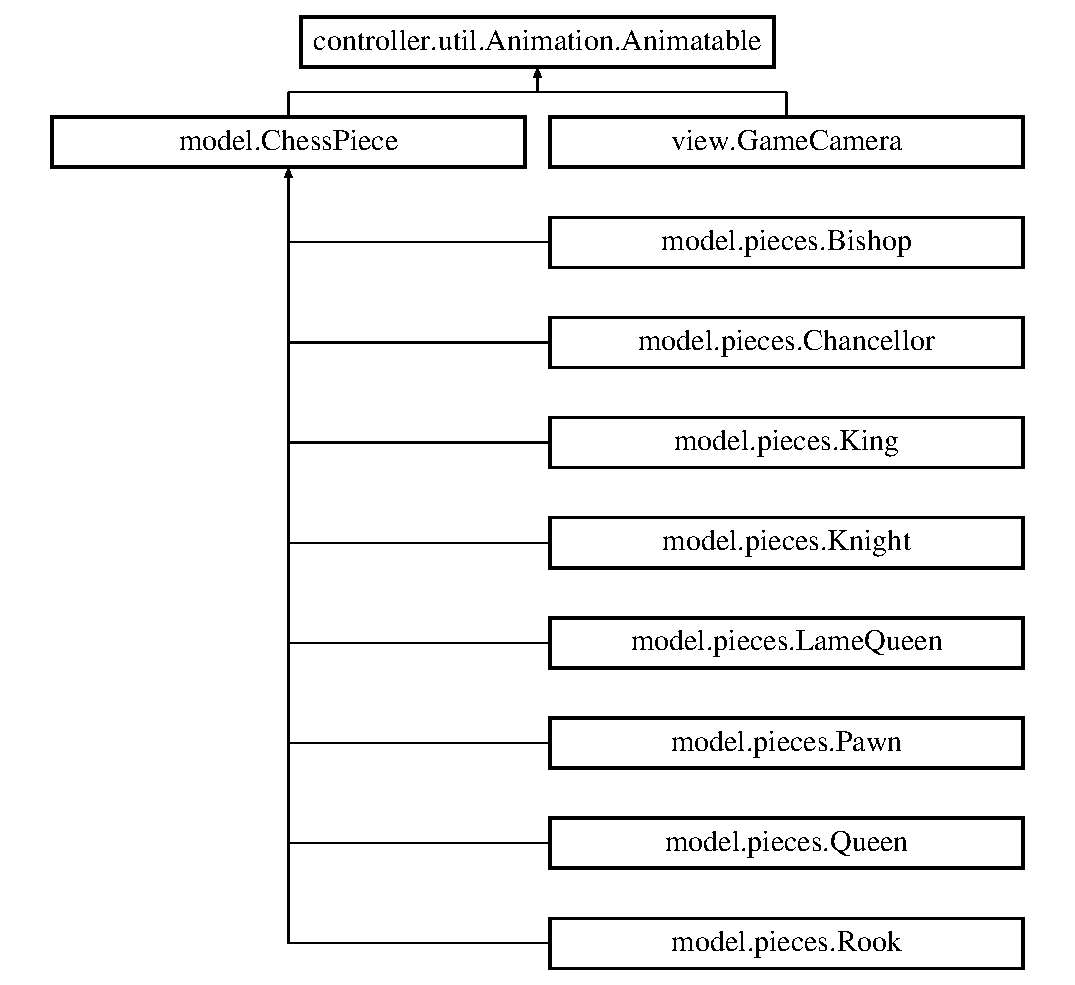
\includegraphics[height=10.000000cm]{interfacecontroller_1_1util_1_1_animation_1_1_animatable}
\end{center}
\end{figure}
\subsection*{Public Member Functions}
\begin{DoxyCompactItemize}
\item 
\hypertarget{interfacecontroller_1_1util_1_1_animation_1_1_animatable_aa2b27febb195a234f498f23a78a4a952}{void {\bfseries set\-Value} (String field\-Name, float value)}\label{interfacecontroller_1_1util_1_1_animation_1_1_animatable_aa2b27febb195a234f498f23a78a4a952}

\end{DoxyCompactItemize}


\subsection{Detailed Description}
Interface that must be implemented by any object that wants to be animated.

\begin{DoxyAuthor}{Author}
Nicholas 
\end{DoxyAuthor}


The documentation for this interface was generated from the following file\-:\begin{DoxyCompactItemize}
\item 
src/controller/util/Animation.\-java\end{DoxyCompactItemize}

\hypertarget{classcontroller_1_1util_1_1_animation}{\section{controller.\-util.\-Animation Class Reference}
\label{classcontroller_1_1util_1_1_animation}\index{controller.\-util.\-Animation@{controller.\-util.\-Animation}}
}
Inheritance diagram for controller.\-util.\-Animation\-:\begin{figure}[H]
\begin{center}
\leavevmode
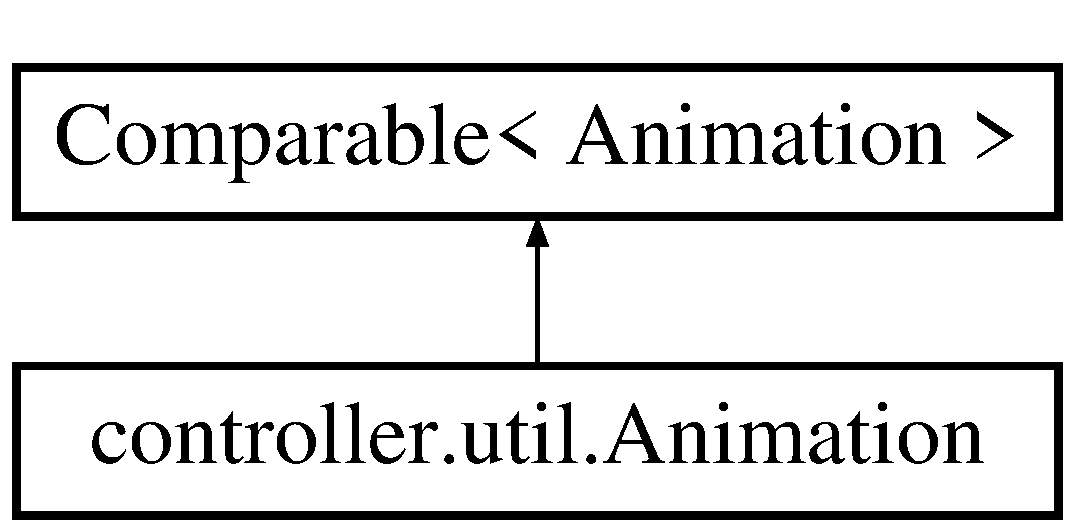
\includegraphics[height=2.000000cm]{classcontroller_1_1util_1_1_animation}
\end{center}
\end{figure}
\subsection*{Classes}
\begin{DoxyCompactItemize}
\item 
interface \hyperlink{interfacecontroller_1_1util_1_1_animation_1_1_animatable}{Animatable}
\end{DoxyCompactItemize}
\subsection*{Public Member Functions}
\begin{DoxyCompactItemize}
\item 
\hyperlink{classcontroller_1_1util_1_1_animation_a43abd777d3c714dd526fca7a3ffde346}{Animation} (\hyperlink{interfacecontroller_1_1util_1_1_animation_1_1_animatable}{Animatable} \-\_\-object, String \-\_\-fieled\-Name, float \-\_\-start\-Val, float \-\_\-end\-Val, float \-\_\-time)
\item 
boolean \hyperlink{classcontroller_1_1util_1_1_animation_a4f4b2dfafe34749665dde788be0ca3d4}{step\-Animation} (float \-\_\-delta\-Time)
\item 
\hypertarget{classcontroller_1_1util_1_1_animation_ac628a796ed83e7d5594d61f27f29b5de}{int {\bfseries compare\-To} (\hyperlink{classcontroller_1_1util_1_1_animation}{Animation} arg0)}\label{classcontroller_1_1util_1_1_animation_ac628a796ed83e7d5594d61f27f29b5de}

\item 
\hypertarget{classcontroller_1_1util_1_1_animation_afba5245ec966e222812ebfa7f473688e}{boolean {\bfseries equals} (Object arg0)}\label{classcontroller_1_1util_1_1_animation_afba5245ec966e222812ebfa7f473688e}

\end{DoxyCompactItemize}


\subsection{Detailed Description}
Defines a basic linear interpolation animation, which is updated by a delta\-\_\-t in the gameloop. This class works by calling the set\-Value() method of the \hyperlink{interfacecontroller_1_1util_1_1_animation_1_1_animatable}{Animatable} object passed in

\begin{DoxyAuthor}{Author}
Nicholas 
\end{DoxyAuthor}


\subsection{Constructor \& Destructor Documentation}
\hypertarget{classcontroller_1_1util_1_1_animation_a43abd777d3c714dd526fca7a3ffde346}{\index{controller\-::util\-::\-Animation@{controller\-::util\-::\-Animation}!Animation@{Animation}}
\index{Animation@{Animation}!controller::util::Animation@{controller\-::util\-::\-Animation}}
\subsubsection[{Animation}]{\setlength{\rightskip}{0pt plus 5cm}controller.\-util.\-Animation.\-Animation (
\begin{DoxyParamCaption}
\item[{{\bf Animatable}}]{\-\_\-object, }
\item[{String}]{\-\_\-fieled\-Name, }
\item[{float}]{\-\_\-start\-Val, }
\item[{float}]{\-\_\-end\-Val, }
\item[{float}]{\-\_\-time}
\end{DoxyParamCaption}
)}}\label{classcontroller_1_1util_1_1_animation_a43abd777d3c714dd526fca7a3ffde346}
Constructs an \hyperlink{classcontroller_1_1util_1_1_animation}{Animation} object that will continually set the value of the object passed in.


\begin{DoxyParams}{Parameters}
{\em \-\_\-object} & Object on which the animation is being performed on \\
\hline
{\em \-\_\-name} & The name of the field in the object that is being updated \\
\hline
{\em \-\_\-start\-Val} & The starting value of the object's field \\
\hline
{\em \-\_\-end\-Val} & The ending value of the object's field \\
\hline
{\em \-\_\-time} & The time of the animation \\
\hline
\end{DoxyParams}


\subsection{Member Function Documentation}
\hypertarget{classcontroller_1_1util_1_1_animation_a4f4b2dfafe34749665dde788be0ca3d4}{\index{controller\-::util\-::\-Animation@{controller\-::util\-::\-Animation}!step\-Animation@{step\-Animation}}
\index{step\-Animation@{step\-Animation}!controller::util::Animation@{controller\-::util\-::\-Animation}}
\subsubsection[{step\-Animation}]{\setlength{\rightskip}{0pt plus 5cm}boolean controller.\-util.\-Animation.\-step\-Animation (
\begin{DoxyParamCaption}
\item[{float}]{\-\_\-delta\-Time}
\end{DoxyParamCaption}
)}}\label{classcontroller_1_1util_1_1_animation_a4f4b2dfafe34749665dde788be0ca3d4}
Steps this animation by \-\_\-delta\-Time, which will result in the object's value being updated by +value\-Step


\begin{DoxyParams}{Parameters}
{\em \-\_\-delta\-Time} & The time step \\
\hline
\end{DoxyParams}
\begin{DoxyReturn}{Returns}
true if the animation has finished, false otherwise 
\end{DoxyReturn}


The documentation for this class was generated from the following file\-:\begin{DoxyCompactItemize}
\item 
src/controller/util/Animation.\-java\end{DoxyCompactItemize}

\hypertarget{classview_1_1loaders_1_1_asset_loader}{\section{view.\-loaders.\-Asset\-Loader Class Reference}
\label{classview_1_1loaders_1_1_asset_loader}\index{view.\-loaders.\-Asset\-Loader@{view.\-loaders.\-Asset\-Loader}}
}
\subsection*{Public Member Functions}
\begin{DoxyCompactItemize}
\item 
void \hyperlink{classview_1_1loaders_1_1_asset_loader_af3230113bdf84d76dd268fbcb6deed6e}{load\-Chess\-Models} (G\-L2 gl)
\item 
void \hyperlink{classview_1_1loaders_1_1_asset_loader_af536a1f7b19c6aa4b1848836df715224}{add\-Model} (\hyperlink{classview_1_1loaders_1_1structures_1_1_model}{Model} model, String name)
\item 
\hyperlink{classview_1_1loaders_1_1structures_1_1_model}{Model} \hyperlink{classview_1_1loaders_1_1_asset_loader_a302d4aefd1e5d3ddd6393da2f99fca1b}{get\-Model} (String name)
\item 
void \hyperlink{classview_1_1loaders_1_1_asset_loader_a5a2978cb6e28a04b8ae1fda0dc912a4c}{load\-Chess\-Textures} (G\-L2 gl)  throws G\-L\-Exception, I\-O\-Exception 
\item 
void \hyperlink{classview_1_1loaders_1_1_asset_loader_a091b9979691c6341a486852e98ff7020}{bind\-Texture} (G\-L2 gl, String name)
\item 
void \hyperlink{classview_1_1loaders_1_1_asset_loader_a5bd7d43403033a835784a346ef80aa53}{load\-Shader} (G\-L2 gl, String path, String name)  throws I\-O\-Exception 
\end{DoxyCompactItemize}
\subsection*{Static Public Member Functions}
\begin{DoxyCompactItemize}
\item 
static \hyperlink{classview_1_1loaders_1_1_asset_loader}{Asset\-Loader} \hyperlink{classview_1_1loaders_1_1_asset_loader_a69d45bb647b18f83fc39e1635ff1f813}{get\-Instance} ()
\end{DoxyCompactItemize}


\subsection{Detailed Description}
Utility class used for loading the required resources for this project including textures, shaders, and models. This class uses the Singleton design pattern \begin{DoxyAuthor}{Author}
Nicholas 
\end{DoxyAuthor}


\subsection{Member Function Documentation}
\hypertarget{classview_1_1loaders_1_1_asset_loader_af536a1f7b19c6aa4b1848836df715224}{\index{view\-::loaders\-::\-Asset\-Loader@{view\-::loaders\-::\-Asset\-Loader}!add\-Model@{add\-Model}}
\index{add\-Model@{add\-Model}!view::loaders::AssetLoader@{view\-::loaders\-::\-Asset\-Loader}}
\subsubsection[{add\-Model}]{\setlength{\rightskip}{0pt plus 5cm}void view.\-loaders.\-Asset\-Loader.\-add\-Model (
\begin{DoxyParamCaption}
\item[{{\bf Model}}]{model, }
\item[{String}]{name}
\end{DoxyParamCaption}
)}}\label{classview_1_1loaders_1_1_asset_loader_af536a1f7b19c6aa4b1848836df715224}
Adds an in application built model, which is used by the Board classes, to add their dynamically created models


\begin{DoxyParams}{Parameters}
{\em model} & \\
\hline
{\em name} & \\
\hline
\end{DoxyParams}
\hypertarget{classview_1_1loaders_1_1_asset_loader_a091b9979691c6341a486852e98ff7020}{\index{view\-::loaders\-::\-Asset\-Loader@{view\-::loaders\-::\-Asset\-Loader}!bind\-Texture@{bind\-Texture}}
\index{bind\-Texture@{bind\-Texture}!view::loaders::AssetLoader@{view\-::loaders\-::\-Asset\-Loader}}
\subsubsection[{bind\-Texture}]{\setlength{\rightskip}{0pt plus 5cm}void view.\-loaders.\-Asset\-Loader.\-bind\-Texture (
\begin{DoxyParamCaption}
\item[{G\-L2}]{gl, }
\item[{String}]{name}
\end{DoxyParamCaption}
)}}\label{classview_1_1loaders_1_1_asset_loader_a091b9979691c6341a486852e98ff7020}
Bind the texture supplied by the name, if it is not the current one bound.


\begin{DoxyParams}{Parameters}
{\em gl} & \\
\hline
{\em name} & \\
\hline
\end{DoxyParams}
\hypertarget{classview_1_1loaders_1_1_asset_loader_a69d45bb647b18f83fc39e1635ff1f813}{\index{view\-::loaders\-::\-Asset\-Loader@{view\-::loaders\-::\-Asset\-Loader}!get\-Instance@{get\-Instance}}
\index{get\-Instance@{get\-Instance}!view::loaders::AssetLoader@{view\-::loaders\-::\-Asset\-Loader}}
\subsubsection[{get\-Instance}]{\setlength{\rightskip}{0pt plus 5cm}static {\bf Asset\-Loader} view.\-loaders.\-Asset\-Loader.\-get\-Instance (
\begin{DoxyParamCaption}
{}
\end{DoxyParamCaption}
)\hspace{0.3cm}{\ttfamily [static]}}}\label{classview_1_1loaders_1_1_asset_loader_a69d45bb647b18f83fc39e1635ff1f813}
Returns the only created object of the \hyperlink{classview_1_1loaders_1_1_asset_loader}{Asset\-Loader} class, and if no object exists yet create one.

\begin{DoxyReturn}{Returns}
a reference to the only \hyperlink{classview_1_1loaders_1_1_asset_loader}{Asset\-Loader} class 
\end{DoxyReturn}
\hypertarget{classview_1_1loaders_1_1_asset_loader_a302d4aefd1e5d3ddd6393da2f99fca1b}{\index{view\-::loaders\-::\-Asset\-Loader@{view\-::loaders\-::\-Asset\-Loader}!get\-Model@{get\-Model}}
\index{get\-Model@{get\-Model}!view::loaders::AssetLoader@{view\-::loaders\-::\-Asset\-Loader}}
\subsubsection[{get\-Model}]{\setlength{\rightskip}{0pt plus 5cm}{\bf Model} view.\-loaders.\-Asset\-Loader.\-get\-Model (
\begin{DoxyParamCaption}
\item[{String}]{name}
\end{DoxyParamCaption}
)}}\label{classview_1_1loaders_1_1_asset_loader_a302d4aefd1e5d3ddd6393da2f99fca1b}

\begin{DoxyParams}{Parameters}
{\em name} & \\
\hline
\end{DoxyParams}
\begin{DoxyReturn}{Returns}
returns the model for the name 
\end{DoxyReturn}
\hypertarget{classview_1_1loaders_1_1_asset_loader_af3230113bdf84d76dd268fbcb6deed6e}{\index{view\-::loaders\-::\-Asset\-Loader@{view\-::loaders\-::\-Asset\-Loader}!load\-Chess\-Models@{load\-Chess\-Models}}
\index{load\-Chess\-Models@{load\-Chess\-Models}!view::loaders::AssetLoader@{view\-::loaders\-::\-Asset\-Loader}}
\subsubsection[{load\-Chess\-Models}]{\setlength{\rightskip}{0pt plus 5cm}void view.\-loaders.\-Asset\-Loader.\-load\-Chess\-Models (
\begin{DoxyParamCaption}
\item[{G\-L2}]{gl}
\end{DoxyParamCaption}
)}}\label{classview_1_1loaders_1_1_asset_loader_af3230113bdf84d76dd268fbcb6deed6e}
Loads a basic model file, with the format (vertex, normal, texture\-Coord)\par
"


\begin{DoxyParams}{Parameters}
{\em gl} & \\
\hline
{\em file} & the directory of all the models \\
\hline
\end{DoxyParams}
\hypertarget{classview_1_1loaders_1_1_asset_loader_a5a2978cb6e28a04b8ae1fda0dc912a4c}{\index{view\-::loaders\-::\-Asset\-Loader@{view\-::loaders\-::\-Asset\-Loader}!load\-Chess\-Textures@{load\-Chess\-Textures}}
\index{load\-Chess\-Textures@{load\-Chess\-Textures}!view::loaders::AssetLoader@{view\-::loaders\-::\-Asset\-Loader}}
\subsubsection[{load\-Chess\-Textures}]{\setlength{\rightskip}{0pt plus 5cm}void view.\-loaders.\-Asset\-Loader.\-load\-Chess\-Textures (
\begin{DoxyParamCaption}
\item[{G\-L2}]{gl}
\end{DoxyParamCaption}
) throws G\-L\-Exception, I\-O\-Exception}}\label{classview_1_1loaders_1_1_asset_loader_a5a2978cb6e28a04b8ae1fda0dc912a4c}
Load all the textures in the file supplied


\begin{DoxyParams}{Parameters}
{\em gl} & \\
\hline
{\em dir} & the file containing the textures \\
\hline
\end{DoxyParams}

\begin{DoxyExceptions}{Exceptions}
{\em I\-O\-Exception} & \\
\hline
{\em G\-L\-Exception} & \\
\hline
\end{DoxyExceptions}
\hypertarget{classview_1_1loaders_1_1_asset_loader_a5bd7d43403033a835784a346ef80aa53}{\index{view\-::loaders\-::\-Asset\-Loader@{view\-::loaders\-::\-Asset\-Loader}!load\-Shader@{load\-Shader}}
\index{load\-Shader@{load\-Shader}!view::loaders::AssetLoader@{view\-::loaders\-::\-Asset\-Loader}}
\subsubsection[{load\-Shader}]{\setlength{\rightskip}{0pt plus 5cm}void view.\-loaders.\-Asset\-Loader.\-load\-Shader (
\begin{DoxyParamCaption}
\item[{G\-L2}]{gl, }
\item[{String}]{path, }
\item[{String}]{name}
\end{DoxyParamCaption}
) throws I\-O\-Exception}}\label{classview_1_1loaders_1_1_asset_loader_a5bd7d43403033a835784a346ef80aa53}
Loads a shader file


\begin{DoxyParams}{Parameters}
{\em gl} & \\
\hline
{\em data\-Source} & \\
\hline
\end{DoxyParams}

\begin{DoxyExceptions}{Exceptions}
{\em I\-O\-Exception} & \\
\hline
\end{DoxyExceptions}


The documentation for this class was generated from the following file\-:\begin{DoxyCompactItemize}
\item 
src/view/loaders/Asset\-Loader.\-java\end{DoxyCompactItemize}

\hypertarget{classmodel_1_1pieces_1_1_bishop}{\section{model.\-pieces.\-Bishop Class Reference}
\label{classmodel_1_1pieces_1_1_bishop}\index{model.\-pieces.\-Bishop@{model.\-pieces.\-Bishop}}
}
Inheritance diagram for model.\-pieces.\-Bishop\-:\begin{figure}[H]
\begin{center}
\leavevmode
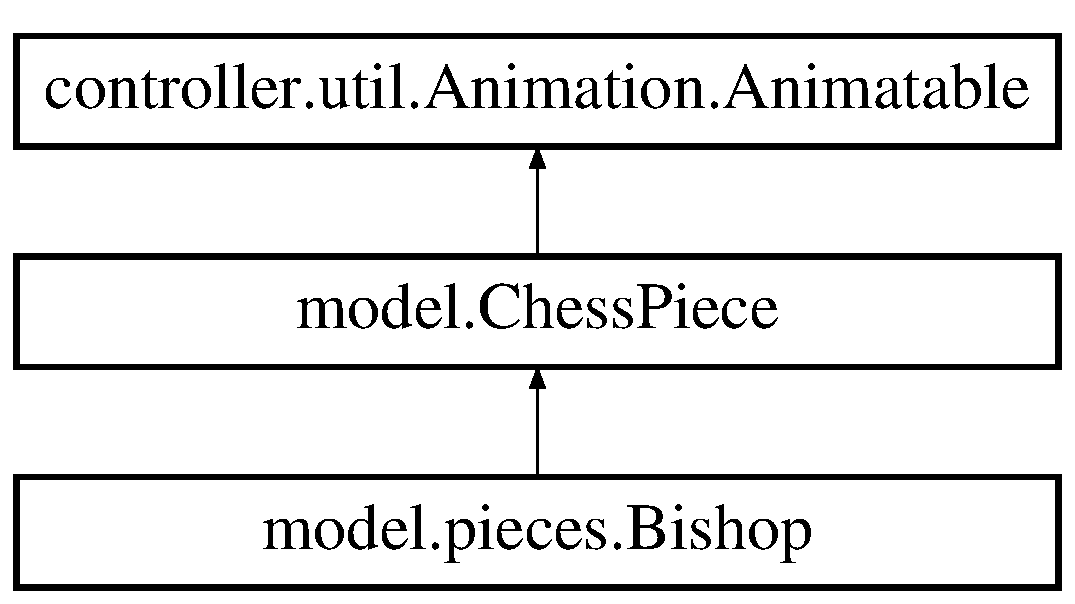
\includegraphics[height=3.000000cm]{classmodel_1_1pieces_1_1_bishop}
\end{center}
\end{figure}
\subsection*{Public Member Functions}
\begin{DoxyCompactItemize}
\item 
\hypertarget{classmodel_1_1pieces_1_1_bishop_ae2668ef3ed3019d746808223561010da}{{\bfseries Bishop} (int x, int y, \hyperlink{classmodel_1_1board_1_1_board}{Board} \-\_\-board, \hyperlink{classcontroller_1_1_player}{Player} \-\_\-player)}\label{classmodel_1_1pieces_1_1_bishop_ae2668ef3ed3019d746808223561010da}

\item 
Array\-List$<$ \hyperlink{classmodel_1_1_chess_move}{Chess\-Move} $>$ \hyperlink{classmodel_1_1pieces_1_1_bishop_a833d5968dbfb775dc72d1cadb68242b3}{get\-Possible\-Moves} ()
\item 
String \hyperlink{classmodel_1_1pieces_1_1_bishop_af15a1172b7ec3d8e895d519f8e540d1c}{get\-Type} ()
\end{DoxyCompactItemize}
\subsection*{Additional Inherited Members}


\subsection{Detailed Description}
Represents a bishop

\begin{DoxyAuthor}{Author}
Nicholas 
\end{DoxyAuthor}


\subsection{Member Function Documentation}
\hypertarget{classmodel_1_1pieces_1_1_bishop_a833d5968dbfb775dc72d1cadb68242b3}{\index{model\-::pieces\-::\-Bishop@{model\-::pieces\-::\-Bishop}!get\-Possible\-Moves@{get\-Possible\-Moves}}
\index{get\-Possible\-Moves@{get\-Possible\-Moves}!model::pieces::Bishop@{model\-::pieces\-::\-Bishop}}
\subsubsection[{get\-Possible\-Moves}]{\setlength{\rightskip}{0pt plus 5cm}Array\-List$<${\bf Chess\-Move}$>$ model.\-pieces.\-Bishop.\-get\-Possible\-Moves (
\begin{DoxyParamCaption}
{}
\end{DoxyParamCaption}
)\hspace{0.3cm}{\ttfamily [virtual]}}}\label{classmodel_1_1pieces_1_1_bishop_a833d5968dbfb775dc72d1cadb68242b3}
Returns all the diagonal moves that the bishop can capture/move 

Implements \hyperlink{classmodel_1_1_chess_piece_a39d690c52727de4a27d2faee4e8b1ac7}{model.\-Chess\-Piece}.

\hypertarget{classmodel_1_1pieces_1_1_bishop_af15a1172b7ec3d8e895d519f8e540d1c}{\index{model\-::pieces\-::\-Bishop@{model\-::pieces\-::\-Bishop}!get\-Type@{get\-Type}}
\index{get\-Type@{get\-Type}!model::pieces::Bishop@{model\-::pieces\-::\-Bishop}}
\subsubsection[{get\-Type}]{\setlength{\rightskip}{0pt plus 5cm}String model.\-pieces.\-Bishop.\-get\-Type (
\begin{DoxyParamCaption}
{}
\end{DoxyParamCaption}
)\hspace{0.3cm}{\ttfamily [virtual]}}}\label{classmodel_1_1pieces_1_1_bishop_af15a1172b7ec3d8e895d519f8e540d1c}
Used to determine a pieces type without using reflection (ie instanceof)

\begin{DoxyReturn}{Returns}
A string that contains the name of the piece, ie the \hyperlink{classmodel_1_1pieces_1_1_pawn}{Pawn} class would return \char`\"{}\-Pawn\char`\"{} 
\end{DoxyReturn}


Implements \hyperlink{classmodel_1_1_chess_piece_a68308e2fa0fe868f7386d40c6cd925df}{model.\-Chess\-Piece}.



The documentation for this class was generated from the following file\-:\begin{DoxyCompactItemize}
\item 
src/model/pieces/Bishop.\-java\end{DoxyCompactItemize}

\hypertarget{classmodel_1_1board_1_1_board}{\section{model.\-board.\-Board Class Reference}
\label{classmodel_1_1board_1_1_board}\index{model.\-board.\-Board@{model.\-board.\-Board}}
}
Inheritance diagram for model.\-board.\-Board\-:\begin{figure}[H]
\begin{center}
\leavevmode
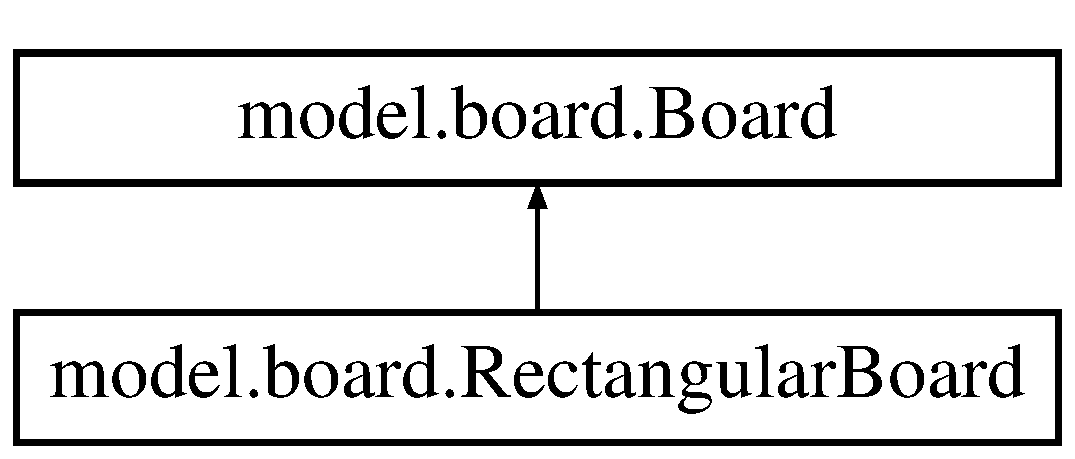
\includegraphics[height=2.000000cm]{classmodel_1_1board_1_1_board}
\end{center}
\end{figure}
\subsection*{Public Member Functions}
\begin{DoxyCompactItemize}
\item 
abstract \hyperlink{classview_1_1loaders_1_1structures_1_1_model}{Model} \hyperlink{classmodel_1_1board_1_1_board_a27db942b8b62795b8e8e615c2e39b432}{generate\-Board\-Model} ()
\item 
abstract \hyperlink{classview_1_1loaders_1_1structures_1_1_model}{Model} \hyperlink{classmodel_1_1board_1_1_board_a40de2efe23a2a995394e7223a5c85896}{generate\-Tile\-Model} ()
\item 
abstract String \hyperlink{classmodel_1_1board_1_1_board_a6d5675d9156c70de1c08842cea728749}{get\-Type} ()
\item 
abstract Point2\-D.\-Float \hyperlink{classmodel_1_1board_1_1_board_a2e1be001e288e4501a80844b45024a94}{get\-Render\-Position} (Point loc)
\item 
abstract Point \hyperlink{classmodel_1_1board_1_1_board_adbfd9f6c5999ef5a9705abbfadb8c924}{get\-Board\-Position} (Point2\-D.\-Float render\-Point)
\item 
abstract \hyperlink{classmodel_1_1_chess_piece}{Chess\-Piece} \hyperlink{classmodel_1_1board_1_1_board_a430d840f3362de265f54f815bf02893a}{get\-Tile} (int x, int y)
\item 
abstract \hyperlink{classmodel_1_1_chess_piece}{Chess\-Piece} \hyperlink{classmodel_1_1board_1_1_board_a2ee2df58c449ad4251b26266a1c326d7}{set\-Tile} (\hyperlink{classmodel_1_1_chess_piece}{Chess\-Piece} piece, int x, int y)
\item 
abstract boolean \hyperlink{classmodel_1_1board_1_1_board_a7c4c6d14284584b90dd969ba80bda496}{is\-In\-Bounds} (int x, int y)
\item 
abstract boolean \hyperlink{classmodel_1_1board_1_1_board_ae6c8e172c9bb977b3be9f023736a3f80}{has\-Enemy\-Piece} (int x, int y, \hyperlink{classcontroller_1_1_player}{Player} attacker)
\item 
abstract boolean \hyperlink{classmodel_1_1board_1_1_board_abbfd0ab523b5a8953556ff6aad8d42c6}{is\-Movable\-Tile} (int x, int y, \hyperlink{classcontroller_1_1_player}{Player} attacker, boolean can\-Capture)
\item 
abstract Array\-List$<$ Point $>$ \hyperlink{classmodel_1_1board_1_1_board_adae13d194d3acf1ae586162cf8ae6786}{get\-Adjacent\-Rank\-File\-Tiles} (int x, int y)
\item 
abstract Array\-List$<$ Point $>$ \hyperlink{classmodel_1_1board_1_1_board_a5b3cecdde64a0a00a538fbc69e578f9c}{get\-Adjacent\-Diagonal\-Tiles} (int x, int y)
\item 
abstract Array\-List$<$ Point $>$ \hyperlink{classmodel_1_1board_1_1_board_ad65a4ec84fc3dad46f5b2f1e97ecc1b0}{get\-Knight\-Moves} (int x, int y)
\item 
abstract Array\-List$<$ Point $>$ \hyperlink{classmodel_1_1board_1_1_board_a4bd4b119f6f5669aaa2aab456056cd92}{get\-Pawn\-Moves} (int x, int y, \hyperlink{classmodel_1_1pieces_1_1_pawn}{Pawn} pawn)
\item 
abstract Array\-List$<$ Point $>$ \hyperlink{classmodel_1_1board_1_1_board_af75b477308f0cb632cf5e164246cd243}{get\-Pawn\-Attacks} (int x, int y, \hyperlink{classmodel_1_1pieces_1_1_pawn}{Pawn} pawn)
\item 
boolean \hyperlink{classmodel_1_1board_1_1_board_a20d22db525a1d022318b86cbfcd67e16}{is\-In\-Bounds} (Point loc)
\item 
boolean \hyperlink{classmodel_1_1board_1_1_board_a59b3e675b694301aef7e8f2cb6a1a65c}{has\-Enemy\-Piece} (Point loc, \hyperlink{classcontroller_1_1_player}{Player} attacker)
\item 
boolean \hyperlink{classmodel_1_1board_1_1_board_a1c27bff8bfe8cb594e6a576e5529b112}{is\-Movable\-Tile} (Point loc, \hyperlink{classcontroller_1_1_player}{Player} player, boolean can\-Capture)
\item 
Array\-List$<$ Point $>$ \hyperlink{classmodel_1_1board_1_1_board_ac8ffc792e85b09c00923dd593368d107}{get\-Adjacent\-Rank\-File\-Tiles} (Point loc)
\item 
Array\-List$<$ Point $>$ \hyperlink{classmodel_1_1board_1_1_board_a5279618349cb2950d412f6ebd563472b}{get\-Adjacent\-Diagonal\-Tiles} (Point loc)
\item 
boolean \hyperlink{classmodel_1_1board_1_1_board_a95aaad7f4888e5daa665b9b92021cf38}{location\-Pressured} (int x, int y, \hyperlink{classcontroller_1_1_player}{Player} victim)
\item 
boolean \hyperlink{classmodel_1_1board_1_1_board_af9083ec2d9d2193bca4af526f9f8dc99}{location\-Pressured} (Point loc, \hyperlink{classcontroller_1_1_player}{Player} victim)
\item 
boolean \hyperlink{classmodel_1_1board_1_1_board_ae68c80c70dcf77ddcbc81fa793103c31}{is\-Valid\-Move} (\hyperlink{classmodel_1_1_chess_move}{Chess\-Move} move)
\item 
Array\-List$<$ \hyperlink{classmodel_1_1_chess_move}{Chess\-Move} $>$ \hyperlink{classmodel_1_1board_1_1_board_a22726970b60922a6644715ebc441bc6d}{get\-All\-Moves} (\hyperlink{classcontroller_1_1_player}{Player} player)
\item 
boolean \hyperlink{classmodel_1_1board_1_1_board_a8e2c1b97adc00c2b91561bed8f79017d}{no\-Possible\-Moves} (\hyperlink{classcontroller_1_1_player}{Player} victim)
\item 
abstract void \hyperlink{classmodel_1_1board_1_1_board_a2680e928007fbd344f4640e053861883}{render} (G\-L2 gl, \hyperlink{classmodel_1_1_chess_piece}{Chess\-Piece} selected\-Piece)
\end{DoxyCompactItemize}
\subsection*{Protected Member Functions}
\begin{DoxyCompactItemize}
\item 
\hypertarget{classmodel_1_1board_1_1_board_a09fc48f686421ff90bf31a4491c133e9}{{\bfseries Board} (\hyperlink{interfacemodel_1_1game__modes_1_1_game_mode}{Game\-Mode} \-\_\-game\-Mode)}\label{classmodel_1_1board_1_1_board_a09fc48f686421ff90bf31a4491c133e9}

\end{DoxyCompactItemize}
\subsection*{Protected Attributes}
\begin{DoxyCompactItemize}
\item 
\hyperlink{interfacemodel_1_1game__modes_1_1_game_mode}{Game\-Mode} \hyperlink{classmodel_1_1board_1_1_board_aeaec4651b92f0416e70eeeaa4959540d}{game\-Mode}
\end{DoxyCompactItemize}


\subsection{Detailed Description}
Abstract board class that is responsible for all the operations on a chess board. The board is responsible for determining if moves are valid, as well as rendering the whole scene.

\begin{DoxyAuthor}{Author}
Nicholas 
\end{DoxyAuthor}


\subsection{Member Function Documentation}
\hypertarget{classmodel_1_1board_1_1_board_a27db942b8b62795b8e8e615c2e39b432}{\index{model\-::board\-::\-Board@{model\-::board\-::\-Board}!generate\-Board\-Model@{generate\-Board\-Model}}
\index{generate\-Board\-Model@{generate\-Board\-Model}!model::board::Board@{model\-::board\-::\-Board}}
\subsubsection[{generate\-Board\-Model}]{\setlength{\rightskip}{0pt plus 5cm}abstract {\bf Model} model.\-board.\-Board.\-generate\-Board\-Model (
\begin{DoxyParamCaption}
{}
\end{DoxyParamCaption}
)\hspace{0.3cm}{\ttfamily [pure virtual]}}}\label{classmodel_1_1board_1_1_board_a27db942b8b62795b8e8e615c2e39b432}
Generates the 3d model for the board, so that it may be added as a model to Asset\-Loader class. N\-O\-T\-E\-: this method is called automatically by the Game\-Loop during setup and should N\-E\-V\-E\-R be called again. The proper way to access this Model would be Asset\-Loader.\-get\-Instace().get\-Model(\hyperlink{classmodel_1_1board_1_1_board_a6d5675d9156c70de1c08842cea728749}{get\-Type()})

\begin{DoxyReturn}{Returns}
the generated board model 
\end{DoxyReturn}


Implemented in \hyperlink{classmodel_1_1board_1_1_rectangular_board_a62edb43eeaeef48c7fd6994806bfc5a4}{model.\-board.\-Rectangular\-Board}.

\hypertarget{classmodel_1_1board_1_1_board_a40de2efe23a2a995394e7223a5c85896}{\index{model\-::board\-::\-Board@{model\-::board\-::\-Board}!generate\-Tile\-Model@{generate\-Tile\-Model}}
\index{generate\-Tile\-Model@{generate\-Tile\-Model}!model::board::Board@{model\-::board\-::\-Board}}
\subsubsection[{generate\-Tile\-Model}]{\setlength{\rightskip}{0pt plus 5cm}abstract {\bf Model} model.\-board.\-Board.\-generate\-Tile\-Model (
\begin{DoxyParamCaption}
{}
\end{DoxyParamCaption}
)\hspace{0.3cm}{\ttfamily [pure virtual]}}}\label{classmodel_1_1board_1_1_board_a40de2efe23a2a995394e7223a5c85896}
Generates the 3d model for the board, so that it may be added as a model to Asset\-Loader class. N\-O\-T\-E\-: this method is called automatically by the Game\-Loop during setup and should N\-E\-V\-E\-R be called again. The proper way to access this Model would be Asset\-Loader.\-get\-Instace().get\-Model(\hyperlink{classmodel_1_1board_1_1_board_a6d5675d9156c70de1c08842cea728749}{get\-Type()})

\begin{DoxyReturn}{Returns}
the generated board model 
\end{DoxyReturn}


Implemented in \hyperlink{classmodel_1_1board_1_1_rectangular_board_a871d89a154bd3628e00504bd91747109}{model.\-board.\-Rectangular\-Board}.

\hypertarget{classmodel_1_1board_1_1_board_a5b3cecdde64a0a00a538fbc69e578f9c}{\index{model\-::board\-::\-Board@{model\-::board\-::\-Board}!get\-Adjacent\-Diagonal\-Tiles@{get\-Adjacent\-Diagonal\-Tiles}}
\index{get\-Adjacent\-Diagonal\-Tiles@{get\-Adjacent\-Diagonal\-Tiles}!model::board::Board@{model\-::board\-::\-Board}}
\subsubsection[{get\-Adjacent\-Diagonal\-Tiles}]{\setlength{\rightskip}{0pt plus 5cm}abstract Array\-List$<$Point$>$ model.\-board.\-Board.\-get\-Adjacent\-Diagonal\-Tiles (
\begin{DoxyParamCaption}
\item[{int}]{x, }
\item[{int}]{y}
\end{DoxyParamCaption}
)\hspace{0.3cm}{\ttfamily [pure virtual]}}}\label{classmodel_1_1board_1_1_board_a5b3cecdde64a0a00a538fbc69e578f9c}
This method on a rectangular board return 4 positions (top-\/left, top-\/right, bottom-\/left, bottom-\/right) and on a hexagonal 5. This method is best thought of as all the directions a bishop would travel. N\-O\-T\-E\-: these locations may not be in bounds, and must be checked accordingly.


\begin{DoxyParams}{Parameters}
{\em x} & \hyperlink{classmodel_1_1board_1_1_board}{Board} location x \\
\hline
{\em y} & \hyperlink{classmodel_1_1board_1_1_board}{Board} location y \\
\hline
\end{DoxyParams}
\begin{DoxyReturn}{Returns}
an array of all the locations diagonal to the given location 
\end{DoxyReturn}


Implemented in \hyperlink{classmodel_1_1board_1_1_rectangular_board_a43e4180539d99a0b95cf2957b4d43eb2}{model.\-board.\-Rectangular\-Board}.

\hypertarget{classmodel_1_1board_1_1_board_a5279618349cb2950d412f6ebd563472b}{\index{model\-::board\-::\-Board@{model\-::board\-::\-Board}!get\-Adjacent\-Diagonal\-Tiles@{get\-Adjacent\-Diagonal\-Tiles}}
\index{get\-Adjacent\-Diagonal\-Tiles@{get\-Adjacent\-Diagonal\-Tiles}!model::board::Board@{model\-::board\-::\-Board}}
\subsubsection[{get\-Adjacent\-Diagonal\-Tiles}]{\setlength{\rightskip}{0pt plus 5cm}Array\-List$<$Point$>$ model.\-board.\-Board.\-get\-Adjacent\-Diagonal\-Tiles (
\begin{DoxyParamCaption}
\item[{Point}]{loc}
\end{DoxyParamCaption}
)}}\label{classmodel_1_1board_1_1_board_a5279618349cb2950d412f6ebd563472b}
Same as \hyperlink{classmodel_1_1board_1_1_board_a5b3cecdde64a0a00a538fbc69e578f9c}{get\-Adjacent\-Diagonal\-Tiles} 
\begin{DoxyParams}{Parameters}
{\em loc} & \hyperlink{classmodel_1_1board_1_1_board}{Board} location point \\
\hline
\end{DoxyParams}
\hypertarget{classmodel_1_1board_1_1_board_adae13d194d3acf1ae586162cf8ae6786}{\index{model\-::board\-::\-Board@{model\-::board\-::\-Board}!get\-Adjacent\-Rank\-File\-Tiles@{get\-Adjacent\-Rank\-File\-Tiles}}
\index{get\-Adjacent\-Rank\-File\-Tiles@{get\-Adjacent\-Rank\-File\-Tiles}!model::board::Board@{model\-::board\-::\-Board}}
\subsubsection[{get\-Adjacent\-Rank\-File\-Tiles}]{\setlength{\rightskip}{0pt plus 5cm}abstract Array\-List$<$Point$>$ model.\-board.\-Board.\-get\-Adjacent\-Rank\-File\-Tiles (
\begin{DoxyParamCaption}
\item[{int}]{x, }
\item[{int}]{y}
\end{DoxyParamCaption}
)\hspace{0.3cm}{\ttfamily [pure virtual]}}}\label{classmodel_1_1board_1_1_board_adae13d194d3acf1ae586162cf8ae6786}
This method on a rectangular board return 4 positions (left, right, top, bottom) and on a hexagonal 6. This method is best thought of as all the directions a rook would travel. N\-O\-T\-E\-: these locations may not be in bounds, and must be checked accordingly


\begin{DoxyParams}{Parameters}
{\em x} & \hyperlink{classmodel_1_1board_1_1_board}{Board} location x \\
\hline
{\em y} & \hyperlink{classmodel_1_1board_1_1_board}{Board} location y \\
\hline
\end{DoxyParams}
\begin{DoxyReturn}{Returns}
an array of all the locations adjacent to the given location 
\end{DoxyReturn}


Implemented in \hyperlink{classmodel_1_1board_1_1_rectangular_board_a58a8b1a8a8505340bd2e6dd2f3268aaa}{model.\-board.\-Rectangular\-Board}.

\hypertarget{classmodel_1_1board_1_1_board_ac8ffc792e85b09c00923dd593368d107}{\index{model\-::board\-::\-Board@{model\-::board\-::\-Board}!get\-Adjacent\-Rank\-File\-Tiles@{get\-Adjacent\-Rank\-File\-Tiles}}
\index{get\-Adjacent\-Rank\-File\-Tiles@{get\-Adjacent\-Rank\-File\-Tiles}!model::board::Board@{model\-::board\-::\-Board}}
\subsubsection[{get\-Adjacent\-Rank\-File\-Tiles}]{\setlength{\rightskip}{0pt plus 5cm}Array\-List$<$Point$>$ model.\-board.\-Board.\-get\-Adjacent\-Rank\-File\-Tiles (
\begin{DoxyParamCaption}
\item[{Point}]{loc}
\end{DoxyParamCaption}
)}}\label{classmodel_1_1board_1_1_board_ac8ffc792e85b09c00923dd593368d107}
Same as \hyperlink{classmodel_1_1board_1_1_board_adae13d194d3acf1ae586162cf8ae6786}{get\-Adjacent\-Flat\-Tiles} 
\begin{DoxyParams}{Parameters}
{\em loc} & \hyperlink{classmodel_1_1board_1_1_board}{Board} location point \\
\hline
\end{DoxyParams}
\hypertarget{classmodel_1_1board_1_1_board_a22726970b60922a6644715ebc441bc6d}{\index{model\-::board\-::\-Board@{model\-::board\-::\-Board}!get\-All\-Moves@{get\-All\-Moves}}
\index{get\-All\-Moves@{get\-All\-Moves}!model::board::Board@{model\-::board\-::\-Board}}
\subsubsection[{get\-All\-Moves}]{\setlength{\rightskip}{0pt plus 5cm}Array\-List$<${\bf Chess\-Move}$>$ model.\-board.\-Board.\-get\-All\-Moves (
\begin{DoxyParamCaption}
\item[{{\bf Player}}]{player}
\end{DoxyParamCaption}
)}}\label{classmodel_1_1board_1_1_board_a22726970b60922a6644715ebc441bc6d}
Returns all the valid moves for the player, see \hyperlink{classmodel_1_1board_1_1_board_ae68c80c70dcf77ddcbc81fa793103c31}{is\-Valid\-Move} for the definition on a valid move


\begin{DoxyParams}{Parameters}
{\em player} & \\
\hline
\end{DoxyParams}
\begin{DoxyReturn}{Returns}
an array of all valid moves 
\end{DoxyReturn}
\hypertarget{classmodel_1_1board_1_1_board_adbfd9f6c5999ef5a9705abbfadb8c924}{\index{model\-::board\-::\-Board@{model\-::board\-::\-Board}!get\-Board\-Position@{get\-Board\-Position}}
\index{get\-Board\-Position@{get\-Board\-Position}!model::board::Board@{model\-::board\-::\-Board}}
\subsubsection[{get\-Board\-Position}]{\setlength{\rightskip}{0pt plus 5cm}abstract Point model.\-board.\-Board.\-get\-Board\-Position (
\begin{DoxyParamCaption}
\item[{Point2\-D.\-Float}]{render\-Point}
\end{DoxyParamCaption}
)\hspace{0.3cm}{\ttfamily [pure virtual]}}}\label{classmodel_1_1board_1_1_board_adbfd9f6c5999ef5a9705abbfadb8c924}
Converts the given 3d location into a tile location, which can be used to access items on the board


\begin{DoxyParams}{Parameters}
{\em render\-Point} & 3d point \\
\hline
\end{DoxyParams}
\begin{DoxyReturn}{Returns}
tile point representation of loc 
\end{DoxyReturn}


Implemented in \hyperlink{classmodel_1_1board_1_1_rectangular_board_aba36dbe678c51dab2bf11f2735122f4a}{model.\-board.\-Rectangular\-Board}.

\hypertarget{classmodel_1_1board_1_1_board_ad65a4ec84fc3dad46f5b2f1e97ecc1b0}{\index{model\-::board\-::\-Board@{model\-::board\-::\-Board}!get\-Knight\-Moves@{get\-Knight\-Moves}}
\index{get\-Knight\-Moves@{get\-Knight\-Moves}!model::board::Board@{model\-::board\-::\-Board}}
\subsubsection[{get\-Knight\-Moves}]{\setlength{\rightskip}{0pt plus 5cm}abstract Array\-List$<$Point$>$ model.\-board.\-Board.\-get\-Knight\-Moves (
\begin{DoxyParamCaption}
\item[{int}]{x, }
\item[{int}]{y}
\end{DoxyParamCaption}
)\hspace{0.3cm}{\ttfamily [pure virtual]}}}\label{classmodel_1_1board_1_1_board_ad65a4ec84fc3dad46f5b2f1e97ecc1b0}
This method on a rectangular board returns 8 positions that form an L shape, and 12 positions on a hexagonal board. N\-O\-T\-E\-: these locations may not be in bounds, and must be checked accordingly


\begin{DoxyParams}{Parameters}
{\em x} & \hyperlink{classmodel_1_1board_1_1_board}{Board} location x \\
\hline
{\em y} & \hyperlink{classmodel_1_1board_1_1_board}{Board} location y \\
\hline
\end{DoxyParams}
\begin{DoxyReturn}{Returns}
an array of all the positions a knight at (x, y) can travel on this board 
\end{DoxyReturn}


Implemented in \hyperlink{classmodel_1_1board_1_1_rectangular_board_a32fbc2d65ed36077c051b05d3c305f1f}{model.\-board.\-Rectangular\-Board}.

\hypertarget{classmodel_1_1board_1_1_board_af75b477308f0cb632cf5e164246cd243}{\index{model\-::board\-::\-Board@{model\-::board\-::\-Board}!get\-Pawn\-Attacks@{get\-Pawn\-Attacks}}
\index{get\-Pawn\-Attacks@{get\-Pawn\-Attacks}!model::board::Board@{model\-::board\-::\-Board}}
\subsubsection[{get\-Pawn\-Attacks}]{\setlength{\rightskip}{0pt plus 5cm}abstract Array\-List$<$Point$>$ model.\-board.\-Board.\-get\-Pawn\-Attacks (
\begin{DoxyParamCaption}
\item[{int}]{x, }
\item[{int}]{y, }
\item[{{\bf Pawn}}]{pawn}
\end{DoxyParamCaption}
)\hspace{0.3cm}{\ttfamily [pure virtual]}}}\label{classmodel_1_1board_1_1_board_af75b477308f0cb632cf5e164246cd243}
This method on a rectangular board returns 2 positions, on a rectangular board these are the 2 diagonals in front, while on a hex board they are the top-\/left and top-\/right adjacent tiles.


\begin{DoxyParams}{Parameters}
{\em x} & \hyperlink{classmodel_1_1board_1_1_board}{Board} location x \\
\hline
{\em y} & \hyperlink{classmodel_1_1board_1_1_board}{Board} location y \\
\hline
\end{DoxyParams}
\begin{DoxyReturn}{Returns}
an array of all the positions a pawn at (x, y) can attack on this board 
\end{DoxyReturn}


Implemented in \hyperlink{classmodel_1_1board_1_1_rectangular_board_a0771a7158bc1c0cbd42c22c95d283f84}{model.\-board.\-Rectangular\-Board}.

\hypertarget{classmodel_1_1board_1_1_board_a4bd4b119f6f5669aaa2aab456056cd92}{\index{model\-::board\-::\-Board@{model\-::board\-::\-Board}!get\-Pawn\-Moves@{get\-Pawn\-Moves}}
\index{get\-Pawn\-Moves@{get\-Pawn\-Moves}!model::board::Board@{model\-::board\-::\-Board}}
\subsubsection[{get\-Pawn\-Moves}]{\setlength{\rightskip}{0pt plus 5cm}abstract Array\-List$<$Point$>$ model.\-board.\-Board.\-get\-Pawn\-Moves (
\begin{DoxyParamCaption}
\item[{int}]{x, }
\item[{int}]{y, }
\item[{{\bf Pawn}}]{pawn}
\end{DoxyParamCaption}
)\hspace{0.3cm}{\ttfamily [pure virtual]}}}\label{classmodel_1_1board_1_1_board_a4bd4b119f6f5669aaa2aab456056cd92}
This method on a rectangular board returns 2 positions if the pawn has not yet moved (the 2 spaces directly in from of the pawn), or 1 move if the pawn has moved The Pawn class is responsible for determining if these locations are valid (ie only one location is valid if it already moved). N\-O\-T\-E\-: these locations may not be in bounds, and must be checked accordingly


\begin{DoxyParams}{Parameters}
{\em x} & \hyperlink{classmodel_1_1board_1_1_board}{Board} location x \\
\hline
{\em y} & \hyperlink{classmodel_1_1board_1_1_board}{Board} location y \\
\hline
\end{DoxyParams}
\begin{DoxyReturn}{Returns}
an array of all the positions a pawn at (x, y) can travel on this board 
\end{DoxyReturn}


Implemented in \hyperlink{classmodel_1_1board_1_1_rectangular_board_a6323cde6b4f30594520205dfab7fbcba}{model.\-board.\-Rectangular\-Board}.

\hypertarget{classmodel_1_1board_1_1_board_a2e1be001e288e4501a80844b45024a94}{\index{model\-::board\-::\-Board@{model\-::board\-::\-Board}!get\-Render\-Position@{get\-Render\-Position}}
\index{get\-Render\-Position@{get\-Render\-Position}!model::board::Board@{model\-::board\-::\-Board}}
\subsubsection[{get\-Render\-Position}]{\setlength{\rightskip}{0pt plus 5cm}abstract Point2\-D.\-Float model.\-board.\-Board.\-get\-Render\-Position (
\begin{DoxyParamCaption}
\item[{Point}]{loc}
\end{DoxyParamCaption}
)\hspace{0.3cm}{\ttfamily [pure virtual]}}}\label{classmodel_1_1board_1_1_board_a2e1be001e288e4501a80844b45024a94}
Converts the given tile location into 3\-D point, that is scaled to the boards size


\begin{DoxyParams}{Parameters}
{\em loc} & tile location \\
\hline
\end{DoxyParams}
\begin{DoxyReturn}{Returns}
3\-D representation of loc 
\end{DoxyReturn}


Implemented in \hyperlink{classmodel_1_1board_1_1_rectangular_board_ab566b2108e82dd874969509cbf4ade03}{model.\-board.\-Rectangular\-Board}.

\hypertarget{classmodel_1_1board_1_1_board_a430d840f3362de265f54f815bf02893a}{\index{model\-::board\-::\-Board@{model\-::board\-::\-Board}!get\-Tile@{get\-Tile}}
\index{get\-Tile@{get\-Tile}!model::board::Board@{model\-::board\-::\-Board}}
\subsubsection[{get\-Tile}]{\setlength{\rightskip}{0pt plus 5cm}abstract {\bf Chess\-Piece} model.\-board.\-Board.\-get\-Tile (
\begin{DoxyParamCaption}
\item[{int}]{x, }
\item[{int}]{y}
\end{DoxyParamCaption}
)\hspace{0.3cm}{\ttfamily [pure virtual]}}}\label{classmodel_1_1board_1_1_board_a430d840f3362de265f54f815bf02893a}
Returns the piece at the given coordinates, as interpreted by the \hyperlink{classmodel_1_1board_1_1_board}{Board} object.


\begin{DoxyParams}{Parameters}
{\em x} & \\
\hline
{\em y} & \\
\hline
\end{DoxyParams}
\begin{DoxyReturn}{Returns}
the \hyperlink{classmodel_1_1_chess_piece}{Chess\-Piece} at the position, null otherwise 
\end{DoxyReturn}


Implemented in \hyperlink{classmodel_1_1board_1_1_rectangular_board_a31120dd8c4e3cb47201a39333945c438}{model.\-board.\-Rectangular\-Board}.

\hypertarget{classmodel_1_1board_1_1_board_a6d5675d9156c70de1c08842cea728749}{\index{model\-::board\-::\-Board@{model\-::board\-::\-Board}!get\-Type@{get\-Type}}
\index{get\-Type@{get\-Type}!model::board::Board@{model\-::board\-::\-Board}}
\subsubsection[{get\-Type}]{\setlength{\rightskip}{0pt plus 5cm}abstract String model.\-board.\-Board.\-get\-Type (
\begin{DoxyParamCaption}
{}
\end{DoxyParamCaption}
)\hspace{0.3cm}{\ttfamily [pure virtual]}}}\label{classmodel_1_1board_1_1_board_a6d5675d9156c70de1c08842cea728749}
String used to identify the type of board. Also used as a unique model name

\begin{DoxyReturn}{Returns}
String used to identify the type of board 
\end{DoxyReturn}


Implemented in \hyperlink{classmodel_1_1board_1_1_rectangular_board_ae31cbebd45c2e8eb4c0f27a2b31ec290}{model.\-board.\-Rectangular\-Board}.

\hypertarget{classmodel_1_1board_1_1_board_ae6c8e172c9bb977b3be9f023736a3f80}{\index{model\-::board\-::\-Board@{model\-::board\-::\-Board}!has\-Enemy\-Piece@{has\-Enemy\-Piece}}
\index{has\-Enemy\-Piece@{has\-Enemy\-Piece}!model::board::Board@{model\-::board\-::\-Board}}
\subsubsection[{has\-Enemy\-Piece}]{\setlength{\rightskip}{0pt plus 5cm}abstract boolean model.\-board.\-Board.\-has\-Enemy\-Piece (
\begin{DoxyParamCaption}
\item[{int}]{x, }
\item[{int}]{y, }
\item[{{\bf Player}}]{attacker}
\end{DoxyParamCaption}
)\hspace{0.3cm}{\ttfamily [pure virtual]}}}\label{classmodel_1_1board_1_1_board_ae6c8e172c9bb977b3be9f023736a3f80}

\begin{DoxyParams}{Parameters}
{\em x} & \hyperlink{classmodel_1_1board_1_1_board}{Board} location x \\
\hline
{\em y} & \hyperlink{classmodel_1_1board_1_1_board}{Board} location y \\
\hline
{\em attacker} & The player making the move \\
\hline
\end{DoxyParams}
\begin{DoxyReturn}{Returns}
true if the tile at (x, y) contains a piece of the opposing player 
\end{DoxyReturn}


Implemented in \hyperlink{classmodel_1_1board_1_1_rectangular_board_addce7bd7a463bb3f279df0022ed4a46f}{model.\-board.\-Rectangular\-Board}.

\hypertarget{classmodel_1_1board_1_1_board_a59b3e675b694301aef7e8f2cb6a1a65c}{\index{model\-::board\-::\-Board@{model\-::board\-::\-Board}!has\-Enemy\-Piece@{has\-Enemy\-Piece}}
\index{has\-Enemy\-Piece@{has\-Enemy\-Piece}!model::board::Board@{model\-::board\-::\-Board}}
\subsubsection[{has\-Enemy\-Piece}]{\setlength{\rightskip}{0pt plus 5cm}boolean model.\-board.\-Board.\-has\-Enemy\-Piece (
\begin{DoxyParamCaption}
\item[{Point}]{loc, }
\item[{{\bf Player}}]{attacker}
\end{DoxyParamCaption}
)}}\label{classmodel_1_1board_1_1_board_a59b3e675b694301aef7e8f2cb6a1a65c}
Same as \hyperlink{}{is\-Attackable} 
\begin{DoxyParams}{Parameters}
{\em loc} & \hyperlink{classmodel_1_1board_1_1_board}{Board} location point \\
\hline
\end{DoxyParams}
\hypertarget{classmodel_1_1board_1_1_board_a7c4c6d14284584b90dd969ba80bda496}{\index{model\-::board\-::\-Board@{model\-::board\-::\-Board}!is\-In\-Bounds@{is\-In\-Bounds}}
\index{is\-In\-Bounds@{is\-In\-Bounds}!model::board::Board@{model\-::board\-::\-Board}}
\subsubsection[{is\-In\-Bounds}]{\setlength{\rightskip}{0pt plus 5cm}abstract boolean model.\-board.\-Board.\-is\-In\-Bounds (
\begin{DoxyParamCaption}
\item[{int}]{x, }
\item[{int}]{y}
\end{DoxyParamCaption}
)\hspace{0.3cm}{\ttfamily [pure virtual]}}}\label{classmodel_1_1board_1_1_board_a7c4c6d14284584b90dd969ba80bda496}

\begin{DoxyParams}{Parameters}
{\em x} & \hyperlink{classmodel_1_1board_1_1_board}{Board} location x \\
\hline
{\em y} & \hyperlink{classmodel_1_1board_1_1_board}{Board} location y \\
\hline
\end{DoxyParams}
\begin{DoxyReturn}{Returns}
true if the given location is within the boards dimensions, false otherwise 
\end{DoxyReturn}


Implemented in \hyperlink{classmodel_1_1board_1_1_rectangular_board_ac462656a89172957d6970476b4e39bf1}{model.\-board.\-Rectangular\-Board}.

\hypertarget{classmodel_1_1board_1_1_board_a20d22db525a1d022318b86cbfcd67e16}{\index{model\-::board\-::\-Board@{model\-::board\-::\-Board}!is\-In\-Bounds@{is\-In\-Bounds}}
\index{is\-In\-Bounds@{is\-In\-Bounds}!model::board::Board@{model\-::board\-::\-Board}}
\subsubsection[{is\-In\-Bounds}]{\setlength{\rightskip}{0pt plus 5cm}boolean model.\-board.\-Board.\-is\-In\-Bounds (
\begin{DoxyParamCaption}
\item[{Point}]{loc}
\end{DoxyParamCaption}
)}}\label{classmodel_1_1board_1_1_board_a20d22db525a1d022318b86cbfcd67e16}
Same as \hyperlink{classmodel_1_1board_1_1_board_a7c4c6d14284584b90dd969ba80bda496}{is\-In\-Bounds} 
\begin{DoxyParams}{Parameters}
{\em loc} & \hyperlink{classmodel_1_1board_1_1_board}{Board} location point \\
\hline
\end{DoxyParams}
\hypertarget{classmodel_1_1board_1_1_board_abbfd0ab523b5a8953556ff6aad8d42c6}{\index{model\-::board\-::\-Board@{model\-::board\-::\-Board}!is\-Movable\-Tile@{is\-Movable\-Tile}}
\index{is\-Movable\-Tile@{is\-Movable\-Tile}!model::board::Board@{model\-::board\-::\-Board}}
\subsubsection[{is\-Movable\-Tile}]{\setlength{\rightskip}{0pt plus 5cm}abstract boolean model.\-board.\-Board.\-is\-Movable\-Tile (
\begin{DoxyParamCaption}
\item[{int}]{x, }
\item[{int}]{y, }
\item[{{\bf Player}}]{attacker, }
\item[{boolean}]{can\-Capture}
\end{DoxyParamCaption}
)\hspace{0.3cm}{\ttfamily [pure virtual]}}}\label{classmodel_1_1board_1_1_board_abbfd0ab523b5a8953556ff6aad8d42c6}

\begin{DoxyParams}{Parameters}
{\em x} & \hyperlink{classmodel_1_1board_1_1_board}{Board} location x \\
\hline
{\em y} & \hyperlink{classmodel_1_1board_1_1_board}{Board} location y \\
\hline
{\em attacker} & The player making the move \\
\hline
{\em can\-Capture} & If a piece is able to capture on the the tile \\
\hline
\end{DoxyParams}
\begin{DoxyReturn}{Returns}
true if the space is open (ie no piece is on the tile) or if the tile contains an enemy piece, and the attacker can capture it 
\end{DoxyReturn}


Implemented in \hyperlink{classmodel_1_1board_1_1_rectangular_board_a4e238edb6b8308d8b561f6418d15e594}{model.\-board.\-Rectangular\-Board}.

\hypertarget{classmodel_1_1board_1_1_board_a1c27bff8bfe8cb594e6a576e5529b112}{\index{model\-::board\-::\-Board@{model\-::board\-::\-Board}!is\-Movable\-Tile@{is\-Movable\-Tile}}
\index{is\-Movable\-Tile@{is\-Movable\-Tile}!model::board::Board@{model\-::board\-::\-Board}}
\subsubsection[{is\-Movable\-Tile}]{\setlength{\rightskip}{0pt plus 5cm}boolean model.\-board.\-Board.\-is\-Movable\-Tile (
\begin{DoxyParamCaption}
\item[{Point}]{loc, }
\item[{{\bf Player}}]{player, }
\item[{boolean}]{can\-Capture}
\end{DoxyParamCaption}
)}}\label{classmodel_1_1board_1_1_board_a1c27bff8bfe8cb594e6a576e5529b112}
Same as \hyperlink{classmodel_1_1board_1_1_board_abbfd0ab523b5a8953556ff6aad8d42c6}{is\-Movable\-Tile} 
\begin{DoxyParams}{Parameters}
{\em loc} & \hyperlink{classmodel_1_1board_1_1_board}{Board} location point \\
\hline
\end{DoxyParams}
\hypertarget{classmodel_1_1board_1_1_board_ae68c80c70dcf77ddcbc81fa793103c31}{\index{model\-::board\-::\-Board@{model\-::board\-::\-Board}!is\-Valid\-Move@{is\-Valid\-Move}}
\index{is\-Valid\-Move@{is\-Valid\-Move}!model::board::Board@{model\-::board\-::\-Board}}
\subsubsection[{is\-Valid\-Move}]{\setlength{\rightskip}{0pt plus 5cm}boolean model.\-board.\-Board.\-is\-Valid\-Move (
\begin{DoxyParamCaption}
\item[{{\bf Chess\-Move}}]{move}
\end{DoxyParamCaption}
)}}\label{classmodel_1_1board_1_1_board_ae68c80c70dcf77ddcbc81fa793103c31}
Determines if this move is valid in the context of the game mode. For example a move that puts a king in check is not valid. This method simulates the move, then asks the game\-Mode to determine if the board is in a valid state. The board is then reset to the original state and the method returns the game mode's response


\begin{DoxyParams}{Parameters}
{\em move} & \\
\hline
\end{DoxyParams}
\begin{DoxyReturn}{Returns}
true if the move is valid in the context of the game\-Mode; 
\end{DoxyReturn}
\hypertarget{classmodel_1_1board_1_1_board_a95aaad7f4888e5daa665b9b92021cf38}{\index{model\-::board\-::\-Board@{model\-::board\-::\-Board}!location\-Pressured@{location\-Pressured}}
\index{location\-Pressured@{location\-Pressured}!model::board::Board@{model\-::board\-::\-Board}}
\subsubsection[{location\-Pressured}]{\setlength{\rightskip}{0pt plus 5cm}boolean model.\-board.\-Board.\-location\-Pressured (
\begin{DoxyParamCaption}
\item[{int}]{x, }
\item[{int}]{y, }
\item[{{\bf Player}}]{victim}
\end{DoxyParamCaption}
)}}\label{classmodel_1_1board_1_1_board_a95aaad7f4888e5daa665b9b92021cf38}

\begin{DoxyParams}{Parameters}
{\em x} & \hyperlink{classmodel_1_1board_1_1_board}{Board} location x \\
\hline
{\em y} & \hyperlink{classmodel_1_1board_1_1_board}{Board} location y \\
\hline
{\em victim} & The player who's piece will be taken \\
\hline
\end{DoxyParams}
\begin{DoxyReturn}{Returns}
true if the victim's piece at (x, y) can be taken by any of the opponents pieces 
\end{DoxyReturn}
\hypertarget{classmodel_1_1board_1_1_board_af9083ec2d9d2193bca4af526f9f8dc99}{\index{model\-::board\-::\-Board@{model\-::board\-::\-Board}!location\-Pressured@{location\-Pressured}}
\index{location\-Pressured@{location\-Pressured}!model::board::Board@{model\-::board\-::\-Board}}
\subsubsection[{location\-Pressured}]{\setlength{\rightskip}{0pt plus 5cm}boolean model.\-board.\-Board.\-location\-Pressured (
\begin{DoxyParamCaption}
\item[{Point}]{loc, }
\item[{{\bf Player}}]{victim}
\end{DoxyParamCaption}
)}}\label{classmodel_1_1board_1_1_board_af9083ec2d9d2193bca4af526f9f8dc99}
Same as \hyperlink{classmodel_1_1board_1_1_board_a95aaad7f4888e5daa665b9b92021cf38}{location\-Capturable} 
\begin{DoxyParams}{Parameters}
{\em loc} & \hyperlink{classmodel_1_1board_1_1_board}{Board} location point \\
\hline
{\em victim} & The player who's piece will be taken \\
\hline
\end{DoxyParams}
\hypertarget{classmodel_1_1board_1_1_board_a8e2c1b97adc00c2b91561bed8f79017d}{\index{model\-::board\-::\-Board@{model\-::board\-::\-Board}!no\-Possible\-Moves@{no\-Possible\-Moves}}
\index{no\-Possible\-Moves@{no\-Possible\-Moves}!model::board::Board@{model\-::board\-::\-Board}}
\subsubsection[{no\-Possible\-Moves}]{\setlength{\rightskip}{0pt plus 5cm}boolean model.\-board.\-Board.\-no\-Possible\-Moves (
\begin{DoxyParamCaption}
\item[{{\bf Player}}]{victim}
\end{DoxyParamCaption}
)}}\label{classmodel_1_1board_1_1_board_a8e2c1b97adc00c2b91561bed8f79017d}
Checks to see if their are any valid moves that can be made


\begin{DoxyParams}{Parameters}
{\em victim} & \\
\hline
\end{DoxyParams}
\begin{DoxyReturn}{Returns}
true if there are any valid moves, false otherwise 
\end{DoxyReturn}
\hypertarget{classmodel_1_1board_1_1_board_a2680e928007fbd344f4640e053861883}{\index{model\-::board\-::\-Board@{model\-::board\-::\-Board}!render@{render}}
\index{render@{render}!model::board::Board@{model\-::board\-::\-Board}}
\subsubsection[{render}]{\setlength{\rightskip}{0pt plus 5cm}abstract void model.\-board.\-Board.\-render (
\begin{DoxyParamCaption}
\item[{G\-L2}]{gl, }
\item[{{\bf Chess\-Piece}}]{selected\-Piece}
\end{DoxyParamCaption}
)\hspace{0.3cm}{\ttfamily [pure virtual]}}}\label{classmodel_1_1board_1_1_board_a2680e928007fbd344f4640e053861883}
Renders the board with the given opengl context. This methods renders the board's mesh, and all the pieces on the board, by repeated calls to Chess\-Piece.\-render(gl);


\begin{DoxyParams}{Parameters}
{\em gl} & \\
\hline
{\em selected\-Piece} & \\
\hline
\end{DoxyParams}


Implemented in \hyperlink{classmodel_1_1board_1_1_rectangular_board_a986119cec9bbcf4699d8c82cd28ede6f}{model.\-board.\-Rectangular\-Board}.

\hypertarget{classmodel_1_1board_1_1_board_a2ee2df58c449ad4251b26266a1c326d7}{\index{model\-::board\-::\-Board@{model\-::board\-::\-Board}!set\-Tile@{set\-Tile}}
\index{set\-Tile@{set\-Tile}!model::board::Board@{model\-::board\-::\-Board}}
\subsubsection[{set\-Tile}]{\setlength{\rightskip}{0pt plus 5cm}abstract {\bf Chess\-Piece} model.\-board.\-Board.\-set\-Tile (
\begin{DoxyParamCaption}
\item[{{\bf Chess\-Piece}}]{piece, }
\item[{int}]{x, }
\item[{int}]{y}
\end{DoxyParamCaption}
)\hspace{0.3cm}{\ttfamily [pure virtual]}}}\label{classmodel_1_1board_1_1_board_a2ee2df58c449ad4251b26266a1c326d7}
Sets the piece to the (x, y) position, and sets the internal board\-Location of the piece. If a piece already existed it is removed from the board, location set to (-\/1, -\/1) and returned


\begin{DoxyParams}{Parameters}
{\em piece} & Piece to be moved \\
\hline
{\em x} & \hyperlink{classmodel_1_1board_1_1_board}{Board} location x \\
\hline
{\em y} & \hyperlink{classmodel_1_1board_1_1_board}{Board} location y \\
\hline
\end{DoxyParams}
\begin{DoxyReturn}{Returns}
the piece that was occupying this tile, null otherwise 
\end{DoxyReturn}


Implemented in \hyperlink{classmodel_1_1board_1_1_rectangular_board_a9a77e49749feb9211f8a70e43d12cf4d}{model.\-board.\-Rectangular\-Board}.



\subsection{Member Data Documentation}
\hypertarget{classmodel_1_1board_1_1_board_aeaec4651b92f0416e70eeeaa4959540d}{\index{model\-::board\-::\-Board@{model\-::board\-::\-Board}!game\-Mode@{game\-Mode}}
\index{game\-Mode@{game\-Mode}!model::board::Board@{model\-::board\-::\-Board}}
\subsubsection[{game\-Mode}]{\setlength{\rightskip}{0pt plus 5cm}{\bf Game\-Mode} model.\-board.\-Board.\-game\-Mode\hspace{0.3cm}{\ttfamily [protected]}}}\label{classmodel_1_1board_1_1_board_aeaec4651b92f0416e70eeeaa4959540d}
Reference to the game\-Mode 

The documentation for this class was generated from the following file\-:\begin{DoxyCompactItemize}
\item 
src/model/board/Board.\-java\end{DoxyCompactItemize}

\hypertarget{classmodel_1_1pieces_1_1_chancellor}{\section{model.\-pieces.\-Chancellor Class Reference}
\label{classmodel_1_1pieces_1_1_chancellor}\index{model.\-pieces.\-Chancellor@{model.\-pieces.\-Chancellor}}
}
Inheritance diagram for model.\-pieces.\-Chancellor\-:\begin{figure}[H]
\begin{center}
\leavevmode
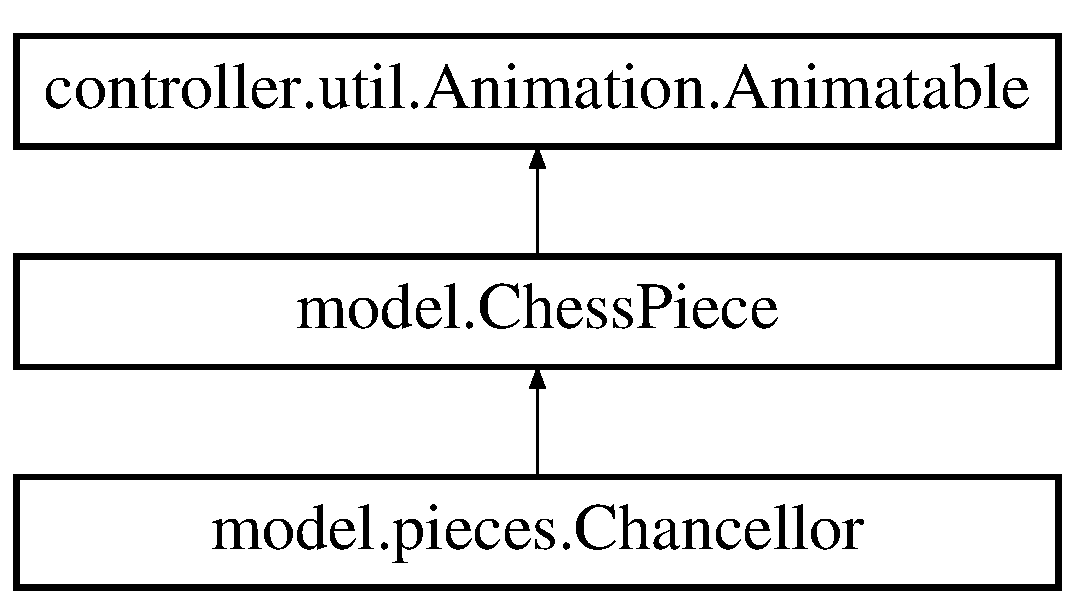
\includegraphics[height=3.000000cm]{classmodel_1_1pieces_1_1_chancellor}
\end{center}
\end{figure}
\subsection*{Public Member Functions}
\begin{DoxyCompactItemize}
\item 
\hypertarget{classmodel_1_1pieces_1_1_chancellor_a5f53a98bd7cd419520e17cd9a692fc15}{{\bfseries Chancellor} (int x, int y, \hyperlink{classmodel_1_1board_1_1_board}{Board} \-\_\-board, \hyperlink{classcontroller_1_1_player}{Player} \-\_\-player)}\label{classmodel_1_1pieces_1_1_chancellor_a5f53a98bd7cd419520e17cd9a692fc15}

\item 
Array\-List$<$ \hyperlink{classmodel_1_1_chess_move}{Chess\-Move} $>$ \hyperlink{classmodel_1_1pieces_1_1_chancellor_a6ec06408734037a969ac9d6d0090894a}{get\-Possible\-Moves} ()
\item 
String \hyperlink{classmodel_1_1pieces_1_1_chancellor_ad8eb0d56c97defeb526ade8f63ee9e90}{get\-Type} ()
\end{DoxyCompactItemize}
\subsection*{Additional Inherited Members}


\subsection{Detailed Description}
Represents a \hyperlink{classmodel_1_1pieces_1_1_chancellor}{Chancellor}. A \hyperlink{classmodel_1_1pieces_1_1_chancellor}{Chancellor} is a hybrid between a rook and a knight.

\begin{DoxyAuthor}{Author}
Nicholas 
\end{DoxyAuthor}


\subsection{Member Function Documentation}
\hypertarget{classmodel_1_1pieces_1_1_chancellor_a6ec06408734037a969ac9d6d0090894a}{\index{model\-::pieces\-::\-Chancellor@{model\-::pieces\-::\-Chancellor}!get\-Possible\-Moves@{get\-Possible\-Moves}}
\index{get\-Possible\-Moves@{get\-Possible\-Moves}!model::pieces::Chancellor@{model\-::pieces\-::\-Chancellor}}
\subsubsection[{get\-Possible\-Moves}]{\setlength{\rightskip}{0pt plus 5cm}Array\-List$<${\bf Chess\-Move}$>$ model.\-pieces.\-Chancellor.\-get\-Possible\-Moves (
\begin{DoxyParamCaption}
{}
\end{DoxyParamCaption}
)\hspace{0.3cm}{\ttfamily [virtual]}}}\label{classmodel_1_1pieces_1_1_chancellor_a6ec06408734037a969ac9d6d0090894a}
Returns all the diagonal moves that the \hyperlink{classmodel_1_1pieces_1_1_chancellor}{Chancellor} can capture/move and all the knigh-\/type moves this piece can capture/move to 

Implements \hyperlink{classmodel_1_1_chess_piece_a39d690c52727de4a27d2faee4e8b1ac7}{model.\-Chess\-Piece}.

\hypertarget{classmodel_1_1pieces_1_1_chancellor_ad8eb0d56c97defeb526ade8f63ee9e90}{\index{model\-::pieces\-::\-Chancellor@{model\-::pieces\-::\-Chancellor}!get\-Type@{get\-Type}}
\index{get\-Type@{get\-Type}!model::pieces::Chancellor@{model\-::pieces\-::\-Chancellor}}
\subsubsection[{get\-Type}]{\setlength{\rightskip}{0pt plus 5cm}String model.\-pieces.\-Chancellor.\-get\-Type (
\begin{DoxyParamCaption}
{}
\end{DoxyParamCaption}
)\hspace{0.3cm}{\ttfamily [virtual]}}}\label{classmodel_1_1pieces_1_1_chancellor_ad8eb0d56c97defeb526ade8f63ee9e90}
Used to determine a pieces type without using reflection (ie instanceof)

\begin{DoxyReturn}{Returns}
A string that contains the name of the piece, ie the \hyperlink{classmodel_1_1pieces_1_1_pawn}{Pawn} class would return \char`\"{}\-Pawn\char`\"{} 
\end{DoxyReturn}


Implements \hyperlink{classmodel_1_1_chess_piece_a68308e2fa0fe868f7386d40c6cd925df}{model.\-Chess\-Piece}.



The documentation for this class was generated from the following file\-:\begin{DoxyCompactItemize}
\item 
src/model/pieces/Chancellor.\-java\end{DoxyCompactItemize}

\hypertarget{classmodel_1_1_chess_move}{\section{model.\-Chess\-Move Class Reference}
\label{classmodel_1_1_chess_move}\index{model.\-Chess\-Move@{model.\-Chess\-Move}}
}
\subsection*{Public Member Functions}
\begin{DoxyCompactItemize}
\item 
\hyperlink{classmodel_1_1_chess_move_afb19b93be0abeee25be72aebe35a6d85}{Chess\-Move} (Point \-\_\-move\-Location, \hyperlink{classmodel_1_1_chess_piece}{Chess\-Piece} \-\_\-piece)
\item 
\hypertarget{classmodel_1_1_chess_move_a8c4f1f2eda79cbf4c904276acf18dc20}{boolean {\bfseries equals} (Object obj)}\label{classmodel_1_1_chess_move_a8c4f1f2eda79cbf4c904276acf18dc20}

\item 
void \hyperlink{classmodel_1_1_chess_move_a284f5700d68e4e8a1d0f89d028a54599}{execute\-Move} (boolean check\-Valid)
\item 
void \hyperlink{classmodel_1_1_chess_move_a15cc98019d1f8b8823b7a4464ca91d5d}{undo\-Move} ()
\item 
\hypertarget{classmodel_1_1_chess_move_ab7763d770448388ba49d6480b6baf7d8}{Point {\bfseries get\-Start\-Location} ()}\label{classmodel_1_1_chess_move_ab7763d770448388ba49d6480b6baf7d8}

\item 
\hypertarget{classmodel_1_1_chess_move_a89ef6d0b7a09792f02af9b6a4f5ef8b4}{Point {\bfseries get\-Move\-Location} ()}\label{classmodel_1_1_chess_move_a89ef6d0b7a09792f02af9b6a4f5ef8b4}

\item 
\hypertarget{classmodel_1_1_chess_move_a5bda891ba042886b6a68182fbd6307f5}{\hyperlink{classmodel_1_1_chess_piece}{Chess\-Piece} {\bfseries get\-Piece} ()}\label{classmodel_1_1_chess_move_a5bda891ba042886b6a68182fbd6307f5}

\item 
\hypertarget{classmodel_1_1_chess_move_ac1c5111a3151395d08bc8a9392acd60d}{Object {\bfseries get\-Captured\-Piece} ()}\label{classmodel_1_1_chess_move_ac1c5111a3151395d08bc8a9392acd60d}

\end{DoxyCompactItemize}


\subsection{Detailed Description}
Basic data object for holding a possible chess move. A chess move is made up of 2 pieces of data, the piece that is moving, and the location the piece will move to

\begin{DoxyAuthor}{Author}
Nicholas 
\end{DoxyAuthor}


\subsection{Constructor \& Destructor Documentation}
\hypertarget{classmodel_1_1_chess_move_afb19b93be0abeee25be72aebe35a6d85}{\index{model\-::\-Chess\-Move@{model\-::\-Chess\-Move}!Chess\-Move@{Chess\-Move}}
\index{Chess\-Move@{Chess\-Move}!model::ChessMove@{model\-::\-Chess\-Move}}
\subsubsection[{Chess\-Move}]{\setlength{\rightskip}{0pt plus 5cm}model.\-Chess\-Move.\-Chess\-Move (
\begin{DoxyParamCaption}
\item[{Point}]{\-\_\-move\-Location, }
\item[{{\bf Chess\-Piece}}]{\-\_\-piece}
\end{DoxyParamCaption}
)}}\label{classmodel_1_1_chess_move_afb19b93be0abeee25be72aebe35a6d85}

\begin{DoxyParams}{Parameters}
{\em \-\_\-move\-Location} & The location being moved to \\
\hline
{\em \-\_\-piece} & The piece being moved \\
\hline
\end{DoxyParams}


\subsection{Member Function Documentation}
\hypertarget{classmodel_1_1_chess_move_a284f5700d68e4e8a1d0f89d028a54599}{\index{model\-::\-Chess\-Move@{model\-::\-Chess\-Move}!execute\-Move@{execute\-Move}}
\index{execute\-Move@{execute\-Move}!model::ChessMove@{model\-::\-Chess\-Move}}
\subsubsection[{execute\-Move}]{\setlength{\rightskip}{0pt plus 5cm}void model.\-Chess\-Move.\-execute\-Move (
\begin{DoxyParamCaption}
\item[{boolean}]{check\-Valid}
\end{DoxyParamCaption}
)}}\label{classmodel_1_1_chess_move_a284f5700d68e4e8a1d0f89d028a54599}
Executes the move if it has not been done yet. Calling this method assumes the move has been checked as valid, otherwise an exception will be thrown. After this move has been completed, caputed\-Piece will be set with the piece that was originally on the tile \hypertarget{classmodel_1_1_chess_move_a15cc98019d1f8b8823b7a4464ca91d5d}{\index{model\-::\-Chess\-Move@{model\-::\-Chess\-Move}!undo\-Move@{undo\-Move}}
\index{undo\-Move@{undo\-Move}!model::ChessMove@{model\-::\-Chess\-Move}}
\subsubsection[{undo\-Move}]{\setlength{\rightskip}{0pt plus 5cm}void model.\-Chess\-Move.\-undo\-Move (
\begin{DoxyParamCaption}
{}
\end{DoxyParamCaption}
)}}\label{classmodel_1_1_chess_move_a15cc98019d1f8b8823b7a4464ca91d5d}
Undoes the move if has not been undone yet. The piece is moved back to its original position, and if there was a piece there already, it is replaced 

The documentation for this class was generated from the following file\-:\begin{DoxyCompactItemize}
\item 
src/model/Chess\-Move.\-java\end{DoxyCompactItemize}

\hypertarget{classmodel_1_1_chess_piece}{\section{model.\-Chess\-Piece Class Reference}
\label{classmodel_1_1_chess_piece}\index{model.\-Chess\-Piece@{model.\-Chess\-Piece}}
}
Inheritance diagram for model.\-Chess\-Piece\-:\begin{figure}[H]
\begin{center}
\leavevmode
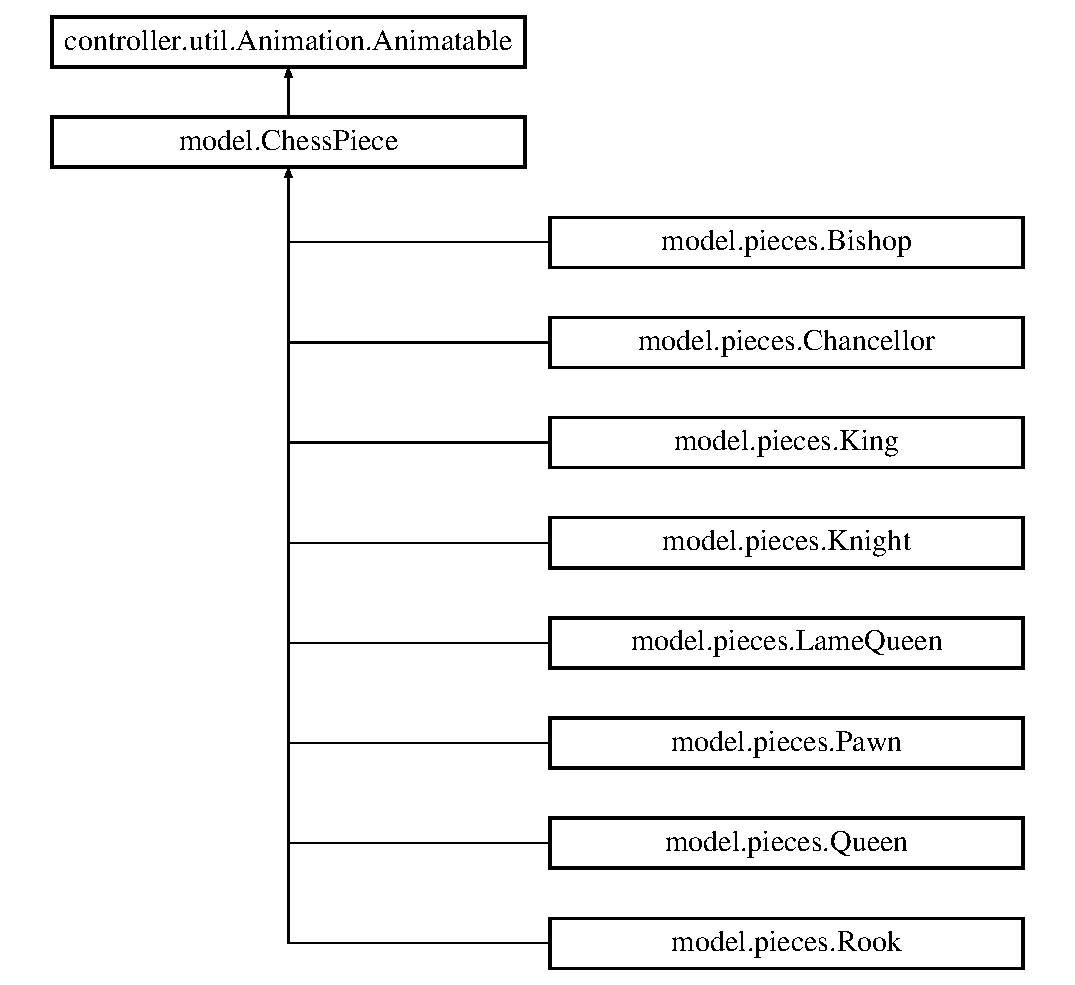
\includegraphics[height=10.000000cm]{classmodel_1_1_chess_piece}
\end{center}
\end{figure}
\subsection*{Public Member Functions}
\begin{DoxyCompactItemize}
\item 
\hyperlink{classmodel_1_1_chess_piece_a67bd82c1cddad23e646cde7505bb5cbb}{Chess\-Piece} (int x, int y, \hyperlink{classmodel_1_1board_1_1_board}{Board} \-\_\-board, \hyperlink{classcontroller_1_1_player}{Player} \-\_\-player)
\item 
\hyperlink{classmodel_1_1_chess_piece}{Chess\-Piece} \hyperlink{classmodel_1_1_chess_piece_af8707e6a255bcb19d1e4936a20e6dc97}{move\-Piece\-To\-Tile} (Point loc, boolean check\-Valid)
\item 
abstract Array\-List$<$ \hyperlink{classmodel_1_1_chess_move}{Chess\-Move} $>$ \hyperlink{classmodel_1_1_chess_piece_a39d690c52727de4a27d2faee4e8b1ac7}{get\-Possible\-Moves} ()
\item 
Array\-List$<$ \hyperlink{classmodel_1_1_chess_move}{Chess\-Move} $>$ \hyperlink{classmodel_1_1_chess_piece_ac47c847341b833c6f3a6fa12c555b859}{get\-Capture\-Moves} ()
\item 
Array\-List$<$ \hyperlink{classmodel_1_1_chess_move}{Chess\-Move} $>$ \hyperlink{classmodel_1_1_chess_piece_a1f7c0c71547a354d71404b8c8a0020ac}{get\-Valid\-Moves} ()
\item 
abstract String \hyperlink{classmodel_1_1_chess_piece_a68308e2fa0fe868f7386d40c6cd925df}{get\-Type} ()
\item 
\hypertarget{classmodel_1_1_chess_piece_ad84ac395de45ea100c9731fb086ef1c0}{void {\bfseries set\-Has\-Moved} (boolean had\-Moved)}\label{classmodel_1_1_chess_piece_ad84ac395de45ea100c9731fb086ef1c0}

\item 
boolean \hyperlink{classmodel_1_1_chess_piece_a085fb407774b223a317d5ad982b88aee}{get\-Has\-Moved} ()
\item 
\hyperlink{classcontroller_1_1_player}{Player} \hyperlink{classmodel_1_1_chess_piece_ac2556be84d4990a806460bbace0610e4}{get\-Player} ()
\item 
void \hyperlink{classmodel_1_1_chess_piece_ad03887b1abfe5503aff3e789f1f15958}{set\-Location} (Point \-\_\-location)
\item 
Point \hyperlink{classmodel_1_1_chess_piece_ae87f373c0666382c92cb644b1a467f6b}{get\-Location} ()
\item 
void \hyperlink{classmodel_1_1_chess_piece_af587b341a0fe842e6aa7562955c33791}{render} (G\-L2 gl)
\item 
void \hyperlink{classmodel_1_1_chess_piece_a9c6576e79cfbc2cc7db4b57569089d1b}{set\-Value} (String field\-Name, float value)
\end{DoxyCompactItemize}
\subsection*{Protected Member Functions}
\begin{DoxyCompactItemize}
\item 
Array\-List$<$ \hyperlink{classmodel_1_1_chess_move}{Chess\-Move} $>$ \hyperlink{classmodel_1_1_chess_piece_ae17e31878bc8896a3dc576c62898c993}{get\-Rank\-File\-Moves} (boolean cont, boolean can\-Capture)
\item 
Array\-List$<$ \hyperlink{classmodel_1_1_chess_move}{Chess\-Move} $>$ \hyperlink{classmodel_1_1_chess_piece_ab8916510321ef5b697b4cd3dd1c7da80}{get\-Diagonal\-Moves} (boolean cont, boolean can\-Capture)
\end{DoxyCompactItemize}
\subsection*{Protected Attributes}
\begin{DoxyCompactItemize}
\item 
Point \hyperlink{classmodel_1_1_chess_piece_a7fc68849278fd30e4c238e8e40d6be8b}{location}
\item 
boolean \hyperlink{classmodel_1_1_chess_piece_ab3cb2b4640d680527a76ee105d233107}{has\-Moved}
\item 
\hyperlink{classcontroller_1_1_player}{Player} \hyperlink{classmodel_1_1_chess_piece_a7c821434522ec5b3f84549ab7b49614f}{player}
\item 
\hyperlink{classmodel_1_1board_1_1_board}{Board} \hyperlink{classmodel_1_1_chess_piece_a41b428c5909b4d5bf0dab321be4cfa56}{board}
\end{DoxyCompactItemize}


\subsection{Detailed Description}
Basic template for any \hyperlink{classmodel_1_1_chess_piece}{Chess\-Piece}, which provides the basic methods to move the Piece.

\begin{DoxyAuthor}{Author}
Nicholas 
\end{DoxyAuthor}


\subsection{Constructor \& Destructor Documentation}
\hypertarget{classmodel_1_1_chess_piece_a67bd82c1cddad23e646cde7505bb5cbb}{\index{model\-::\-Chess\-Piece@{model\-::\-Chess\-Piece}!Chess\-Piece@{Chess\-Piece}}
\index{Chess\-Piece@{Chess\-Piece}!model::ChessPiece@{model\-::\-Chess\-Piece}}
\subsubsection[{Chess\-Piece}]{\setlength{\rightskip}{0pt plus 5cm}model.\-Chess\-Piece.\-Chess\-Piece (
\begin{DoxyParamCaption}
\item[{int}]{x, }
\item[{int}]{y, }
\item[{{\bf Board}}]{\-\_\-board, }
\item[{{\bf Player}}]{\-\_\-player}
\end{DoxyParamCaption}
)}}\label{classmodel_1_1_chess_piece_a67bd82c1cddad23e646cde7505bb5cbb}
Initializes the basic variables of a chess piece and adds it to the board


\begin{DoxyParams}{Parameters}
{\em x} & \\
\hline
{\em y} & \\
\hline
{\em \-\_\-board} & \\
\hline
{\em \-\_\-player} & \\
\hline
\end{DoxyParams}


\subsection{Member Function Documentation}
\hypertarget{classmodel_1_1_chess_piece_ac47c847341b833c6f3a6fa12c555b859}{\index{model\-::\-Chess\-Piece@{model\-::\-Chess\-Piece}!get\-Capture\-Moves@{get\-Capture\-Moves}}
\index{get\-Capture\-Moves@{get\-Capture\-Moves}!model::ChessPiece@{model\-::\-Chess\-Piece}}
\subsubsection[{get\-Capture\-Moves}]{\setlength{\rightskip}{0pt plus 5cm}Array\-List$<${\bf Chess\-Move}$>$ model.\-Chess\-Piece.\-get\-Capture\-Moves (
\begin{DoxyParamCaption}
{}
\end{DoxyParamCaption}
)}}\label{classmodel_1_1_chess_piece_ac47c847341b833c6f3a6fa12c555b859}
Subset of \hyperlink{classmodel_1_1_chess_piece_a39d690c52727de4a27d2faee4e8b1ac7}{get\-Possible\-Moves()} which returns all the moves that result in a capture

\begin{DoxyReturn}{Returns}
An array of all the possible moves this piece can make that result in it taking a piece. 
\end{DoxyReturn}
\hypertarget{classmodel_1_1_chess_piece_ab8916510321ef5b697b4cd3dd1c7da80}{\index{model\-::\-Chess\-Piece@{model\-::\-Chess\-Piece}!get\-Diagonal\-Moves@{get\-Diagonal\-Moves}}
\index{get\-Diagonal\-Moves@{get\-Diagonal\-Moves}!model::ChessPiece@{model\-::\-Chess\-Piece}}
\subsubsection[{get\-Diagonal\-Moves}]{\setlength{\rightskip}{0pt plus 5cm}Array\-List$<${\bf Chess\-Move}$>$ model.\-Chess\-Piece.\-get\-Diagonal\-Moves (
\begin{DoxyParamCaption}
\item[{boolean}]{cont, }
\item[{boolean}]{can\-Capture}
\end{DoxyParamCaption}
)\hspace{0.3cm}{\ttfamily [protected]}}}\label{classmodel_1_1_chess_piece_ab8916510321ef5b697b4cd3dd1c7da80}
Used by pieces such as the bishop, queen and king to get the moves in the diagonal directions of the boards. Will only return all the moves up to (and including) an enemy piece and as long as the piece remains valid


\begin{DoxyParams}{Parameters}
{\em cont} & true returns the list of all moves in the diagonal directions \\
\hline
{\em can\-Capture} & true if this piece can capture \\
\hline
\end{DoxyParams}
\begin{DoxyReturn}{Returns}
an array of the valid moves possible in the diagonal direction 
\end{DoxyReturn}
\hypertarget{classmodel_1_1_chess_piece_a085fb407774b223a317d5ad982b88aee}{\index{model\-::\-Chess\-Piece@{model\-::\-Chess\-Piece}!get\-Has\-Moved@{get\-Has\-Moved}}
\index{get\-Has\-Moved@{get\-Has\-Moved}!model::ChessPiece@{model\-::\-Chess\-Piece}}
\subsubsection[{get\-Has\-Moved}]{\setlength{\rightskip}{0pt plus 5cm}boolean model.\-Chess\-Piece.\-get\-Has\-Moved (
\begin{DoxyParamCaption}
{}
\end{DoxyParamCaption}
)}}\label{classmodel_1_1_chess_piece_a085fb407774b223a317d5ad982b88aee}
\begin{DoxyReturn}{Returns}
true if this piece has moved 
\end{DoxyReturn}
\hypertarget{classmodel_1_1_chess_piece_ae87f373c0666382c92cb644b1a467f6b}{\index{model\-::\-Chess\-Piece@{model\-::\-Chess\-Piece}!get\-Location@{get\-Location}}
\index{get\-Location@{get\-Location}!model::ChessPiece@{model\-::\-Chess\-Piece}}
\subsubsection[{get\-Location}]{\setlength{\rightskip}{0pt plus 5cm}Point model.\-Chess\-Piece.\-get\-Location (
\begin{DoxyParamCaption}
{}
\end{DoxyParamCaption}
)}}\label{classmodel_1_1_chess_piece_ae87f373c0666382c92cb644b1a467f6b}
\begin{DoxyReturn}{Returns}
Point representing the board location of this object 
\end{DoxyReturn}
\hypertarget{classmodel_1_1_chess_piece_ac2556be84d4990a806460bbace0610e4}{\index{model\-::\-Chess\-Piece@{model\-::\-Chess\-Piece}!get\-Player@{get\-Player}}
\index{get\-Player@{get\-Player}!model::ChessPiece@{model\-::\-Chess\-Piece}}
\subsubsection[{get\-Player}]{\setlength{\rightskip}{0pt plus 5cm}{\bf Player} model.\-Chess\-Piece.\-get\-Player (
\begin{DoxyParamCaption}
{}
\end{DoxyParamCaption}
)}}\label{classmodel_1_1_chess_piece_ac2556be84d4990a806460bbace0610e4}
\begin{DoxyReturn}{Returns}
the owning player 
\end{DoxyReturn}
\hypertarget{classmodel_1_1_chess_piece_a39d690c52727de4a27d2faee4e8b1ac7}{\index{model\-::\-Chess\-Piece@{model\-::\-Chess\-Piece}!get\-Possible\-Moves@{get\-Possible\-Moves}}
\index{get\-Possible\-Moves@{get\-Possible\-Moves}!model::ChessPiece@{model\-::\-Chess\-Piece}}
\subsubsection[{get\-Possible\-Moves}]{\setlength{\rightskip}{0pt plus 5cm}abstract Array\-List$<${\bf Chess\-Move}$>$ model.\-Chess\-Piece.\-get\-Possible\-Moves (
\begin{DoxyParamCaption}
{}
\end{DoxyParamCaption}
)\hspace{0.3cm}{\ttfamily [pure virtual]}}}\label{classmodel_1_1_chess_piece_a39d690c52727de4a27d2faee4e8b1ac7}
Overridden by all chess piece classes, which returns an Array of chess moves that this peice can make

\begin{DoxyReturn}{Returns}
An array of all the possible moves this piece can make 
\end{DoxyReturn}


Implemented in \hyperlink{classmodel_1_1pieces_1_1_king_a01079269fe18d60396f980ea099ae7cc}{model.\-pieces.\-King}, \hyperlink{classmodel_1_1pieces_1_1_pawn_aa8a699402fec460438fe1f9d1ba33632}{model.\-pieces.\-Pawn}, \hyperlink{classmodel_1_1pieces_1_1_chancellor_a6ec06408734037a969ac9d6d0090894a}{model.\-pieces.\-Chancellor}, \hyperlink{classmodel_1_1pieces_1_1_knight_a6fc2b0d4bef1c83e84c9351d0b67ae28}{model.\-pieces.\-Knight}, \hyperlink{classmodel_1_1pieces_1_1_lame_queen_a1c58d7e40397c75344909c305f559f7f}{model.\-pieces.\-Lame\-Queen}, \hyperlink{classmodel_1_1pieces_1_1_queen_a94300f345153c441518363f4bef81f9c}{model.\-pieces.\-Queen}, \hyperlink{classmodel_1_1pieces_1_1_rook_acdc88fcdbb81116be30b7f8c8c39e735}{model.\-pieces.\-Rook}, and \hyperlink{classmodel_1_1pieces_1_1_bishop_a833d5968dbfb775dc72d1cadb68242b3}{model.\-pieces.\-Bishop}.

\hypertarget{classmodel_1_1_chess_piece_ae17e31878bc8896a3dc576c62898c993}{\index{model\-::\-Chess\-Piece@{model\-::\-Chess\-Piece}!get\-Rank\-File\-Moves@{get\-Rank\-File\-Moves}}
\index{get\-Rank\-File\-Moves@{get\-Rank\-File\-Moves}!model::ChessPiece@{model\-::\-Chess\-Piece}}
\subsubsection[{get\-Rank\-File\-Moves}]{\setlength{\rightskip}{0pt plus 5cm}Array\-List$<${\bf Chess\-Move}$>$ model.\-Chess\-Piece.\-get\-Rank\-File\-Moves (
\begin{DoxyParamCaption}
\item[{boolean}]{cont, }
\item[{boolean}]{can\-Capture}
\end{DoxyParamCaption}
)\hspace{0.3cm}{\ttfamily [protected]}}}\label{classmodel_1_1_chess_piece_ae17e31878bc8896a3dc576c62898c993}
Used by pieces such as the rook, queen and king to get the moves in the rank-\/file directions of the boards. Will only return all the moves up to (and including) an enemy piece and as long as the piece remains valid


\begin{DoxyParams}{Parameters}
{\em cont} & true returns the list of all moves in the flat directions \\
\hline
{\em can\-Capture} & true if this piece can capture \\
\hline
\end{DoxyParams}
\begin{DoxyReturn}{Returns}
an array of the valid moves possible in the flat direction 
\end{DoxyReturn}
\hypertarget{classmodel_1_1_chess_piece_a68308e2fa0fe868f7386d40c6cd925df}{\index{model\-::\-Chess\-Piece@{model\-::\-Chess\-Piece}!get\-Type@{get\-Type}}
\index{get\-Type@{get\-Type}!model::ChessPiece@{model\-::\-Chess\-Piece}}
\subsubsection[{get\-Type}]{\setlength{\rightskip}{0pt plus 5cm}abstract String model.\-Chess\-Piece.\-get\-Type (
\begin{DoxyParamCaption}
{}
\end{DoxyParamCaption}
)\hspace{0.3cm}{\ttfamily [pure virtual]}}}\label{classmodel_1_1_chess_piece_a68308e2fa0fe868f7386d40c6cd925df}
Used to determine a pieces type without using reflection (ie instanceof)

\begin{DoxyReturn}{Returns}
A string that contains the name of the piece, ie the Pawn class would return \char`\"{}\-Pawn\char`\"{} 
\end{DoxyReturn}


Implemented in \hyperlink{classmodel_1_1pieces_1_1_pawn_a3f4abbb3b7e744569928e51f9a7ace27}{model.\-pieces.\-Pawn}, \hyperlink{classmodel_1_1pieces_1_1_king_aae0c46ac679ce113aa2c5bf64997f618}{model.\-pieces.\-King}, \hyperlink{classmodel_1_1pieces_1_1_knight_a692ba3f99660d39fdbfd55c35d709bed}{model.\-pieces.\-Knight}, \hyperlink{classmodel_1_1pieces_1_1_chancellor_ad8eb0d56c97defeb526ade8f63ee9e90}{model.\-pieces.\-Chancellor}, \hyperlink{classmodel_1_1pieces_1_1_lame_queen_a70f4bafe5a2b59a281b4ef23f3e3680f}{model.\-pieces.\-Lame\-Queen}, \hyperlink{classmodel_1_1pieces_1_1_queen_acf33a9937af8917615b2a53300830af2}{model.\-pieces.\-Queen}, \hyperlink{classmodel_1_1pieces_1_1_bishop_af15a1172b7ec3d8e895d519f8e540d1c}{model.\-pieces.\-Bishop}, and \hyperlink{classmodel_1_1pieces_1_1_rook_a4ff4e4b36a743af9b64de9b53a9e1535}{model.\-pieces.\-Rook}.

\hypertarget{classmodel_1_1_chess_piece_a1f7c0c71547a354d71404b8c8a0020ac}{\index{model\-::\-Chess\-Piece@{model\-::\-Chess\-Piece}!get\-Valid\-Moves@{get\-Valid\-Moves}}
\index{get\-Valid\-Moves@{get\-Valid\-Moves}!model::ChessPiece@{model\-::\-Chess\-Piece}}
\subsubsection[{get\-Valid\-Moves}]{\setlength{\rightskip}{0pt plus 5cm}Array\-List$<${\bf Chess\-Move}$>$ model.\-Chess\-Piece.\-get\-Valid\-Moves (
\begin{DoxyParamCaption}
{}
\end{DoxyParamCaption}
)}}\label{classmodel_1_1_chess_piece_a1f7c0c71547a354d71404b8c8a0020ac}
Subset of \hyperlink{classmodel_1_1_chess_piece_a39d690c52727de4a27d2faee4e8b1ac7}{get\-Possible\-Moves()} which contains all the moves which are valid to the type of game mode. For example, \hyperlink{classmodel_1_1_chess_piece_a39d690c52727de4a27d2faee4e8b1ac7}{get\-Possible\-Moves()} for a king would return the 8 squares around it, while \hyperlink{classmodel_1_1_chess_piece_a1f7c0c71547a354d71404b8c8a0020ac}{get\-Valid\-Moves()} would only return the moves that don't put this king in check (for a standard game)

\begin{DoxyReturn}{Returns}
An array of valid chess moves 
\end{DoxyReturn}
\hypertarget{classmodel_1_1_chess_piece_af8707e6a255bcb19d1e4936a20e6dc97}{\index{model\-::\-Chess\-Piece@{model\-::\-Chess\-Piece}!move\-Piece\-To\-Tile@{move\-Piece\-To\-Tile}}
\index{move\-Piece\-To\-Tile@{move\-Piece\-To\-Tile}!model::ChessPiece@{model\-::\-Chess\-Piece}}
\subsubsection[{move\-Piece\-To\-Tile}]{\setlength{\rightskip}{0pt plus 5cm}{\bf Chess\-Piece} model.\-Chess\-Piece.\-move\-Piece\-To\-Tile (
\begin{DoxyParamCaption}
\item[{Point}]{loc, }
\item[{boolean}]{check\-Valid}
\end{DoxyParamCaption}
)}}\label{classmodel_1_1_chess_piece_af8707e6a255bcb19d1e4936a20e6dc97}
Moves this piece to the position, while internally checking if the moves is valid (by comparing the given location to possible moves)


\begin{DoxyExceptions}{Exceptions}
{\em Illegal\-Argument\-Exception} & if this position cannot move to the given location \\
\hline
\end{DoxyExceptions}

\begin{DoxyParams}{Parameters}
{\em loc} & the location to move to \\
\hline
{\em check\-Valid} & \\
\hline
\end{DoxyParams}
\begin{DoxyReturn}{Returns}
the \hyperlink{classmodel_1_1_chess_piece}{Chess\-Piece} that was at the position original 
\end{DoxyReturn}
\hypertarget{classmodel_1_1_chess_piece_af587b341a0fe842e6aa7562955c33791}{\index{model\-::\-Chess\-Piece@{model\-::\-Chess\-Piece}!render@{render}}
\index{render@{render}!model::ChessPiece@{model\-::\-Chess\-Piece}}
\subsubsection[{render}]{\setlength{\rightskip}{0pt plus 5cm}void model.\-Chess\-Piece.\-render (
\begin{DoxyParamCaption}
\item[{G\-L2}]{gl}
\end{DoxyParamCaption}
)}}\label{classmodel_1_1_chess_piece_af587b341a0fe842e6aa7562955c33791}
Renders this piece to the current open\-G\-L context. The draw\-X and draw\-Y are provided by the board, while the model is retrieved from the Asset\-Loader class. The model used is just the name of the piece (ie \hyperlink{classmodel_1_1_chess_piece_a68308e2fa0fe868f7386d40c6cd925df}{get\-Type()})


\begin{DoxyParams}{Parameters}
{\em gl} & \\
\hline
{\em draw\-X} & \\
\hline
{\em draw\-Z} & \\
\hline
\end{DoxyParams}
\hypertarget{classmodel_1_1_chess_piece_ad03887b1abfe5503aff3e789f1f15958}{\index{model\-::\-Chess\-Piece@{model\-::\-Chess\-Piece}!set\-Location@{set\-Location}}
\index{set\-Location@{set\-Location}!model::ChessPiece@{model\-::\-Chess\-Piece}}
\subsubsection[{set\-Location}]{\setlength{\rightskip}{0pt plus 5cm}void model.\-Chess\-Piece.\-set\-Location (
\begin{DoxyParamCaption}
\item[{Point}]{\-\_\-location}
\end{DoxyParamCaption}
)}}\label{classmodel_1_1_chess_piece_ad03887b1abfe5503aff3e789f1f15958}
Sets this piece's board location to \-\_\-location. N\-O\-T\-E\-: Doe's N\-O\-T change has\-Moved


\begin{DoxyParams}{Parameters}
{\em \-\_\-location} & \\
\hline
\end{DoxyParams}
\hypertarget{classmodel_1_1_chess_piece_a9c6576e79cfbc2cc7db4b57569089d1b}{\index{model\-::\-Chess\-Piece@{model\-::\-Chess\-Piece}!set\-Value@{set\-Value}}
\index{set\-Value@{set\-Value}!model::ChessPiece@{model\-::\-Chess\-Piece}}
\subsubsection[{set\-Value}]{\setlength{\rightskip}{0pt plus 5cm}void model.\-Chess\-Piece.\-set\-Value (
\begin{DoxyParamCaption}
\item[{String}]{field\-Name, }
\item[{float}]{value}
\end{DoxyParamCaption}
)}}\label{classmodel_1_1_chess_piece_a9c6576e79cfbc2cc7db4b57569089d1b}
So that this piece can be animatable, it must overload this method. Two fields can be animated in the class, draw\-Location\-X, and draw\-Location\-Y which are the positions this piece will be rendered on the screen. 

Implements \hyperlink{interfacecontroller_1_1util_1_1_animation_1_1_animatable}{controller.\-util.\-Animation.\-Animatable}.



\subsection{Member Data Documentation}
\hypertarget{classmodel_1_1_chess_piece_a41b428c5909b4d5bf0dab321be4cfa56}{\index{model\-::\-Chess\-Piece@{model\-::\-Chess\-Piece}!board@{board}}
\index{board@{board}!model::ChessPiece@{model\-::\-Chess\-Piece}}
\subsubsection[{board}]{\setlength{\rightskip}{0pt plus 5cm}{\bf Board} model.\-Chess\-Piece.\-board\hspace{0.3cm}{\ttfamily [protected]}}}\label{classmodel_1_1_chess_piece_a41b428c5909b4d5bf0dab321be4cfa56}
Reference to the board \hypertarget{classmodel_1_1_chess_piece_ab3cb2b4640d680527a76ee105d233107}{\index{model\-::\-Chess\-Piece@{model\-::\-Chess\-Piece}!has\-Moved@{has\-Moved}}
\index{has\-Moved@{has\-Moved}!model::ChessPiece@{model\-::\-Chess\-Piece}}
\subsubsection[{has\-Moved}]{\setlength{\rightskip}{0pt plus 5cm}boolean model.\-Chess\-Piece.\-has\-Moved\hspace{0.3cm}{\ttfamily [protected]}}}\label{classmodel_1_1_chess_piece_ab3cb2b4640d680527a76ee105d233107}
If the piece has been used yet \hypertarget{classmodel_1_1_chess_piece_a7fc68849278fd30e4c238e8e40d6be8b}{\index{model\-::\-Chess\-Piece@{model\-::\-Chess\-Piece}!location@{location}}
\index{location@{location}!model::ChessPiece@{model\-::\-Chess\-Piece}}
\subsubsection[{location}]{\setlength{\rightskip}{0pt plus 5cm}Point model.\-Chess\-Piece.\-location\hspace{0.3cm}{\ttfamily [protected]}}}\label{classmodel_1_1_chess_piece_a7fc68849278fd30e4c238e8e40d6be8b}
The board location of the piece \hypertarget{classmodel_1_1_chess_piece_a7c821434522ec5b3f84549ab7b49614f}{\index{model\-::\-Chess\-Piece@{model\-::\-Chess\-Piece}!player@{player}}
\index{player@{player}!model::ChessPiece@{model\-::\-Chess\-Piece}}
\subsubsection[{player}]{\setlength{\rightskip}{0pt plus 5cm}{\bf Player} model.\-Chess\-Piece.\-player\hspace{0.3cm}{\ttfamily [protected]}}}\label{classmodel_1_1_chess_piece_a7c821434522ec5b3f84549ab7b49614f}
The player owning this piece 

The documentation for this class was generated from the following file\-:\begin{DoxyCompactItemize}
\item 
src/model/Chess\-Piece.\-java\end{DoxyCompactItemize}

\hypertarget{classview_1_1_game_camera}{\section{view.\-Game\-Camera Class Reference}
\label{classview_1_1_game_camera}\index{view.\-Game\-Camera@{view.\-Game\-Camera}}
}
Inheritance diagram for view.\-Game\-Camera\-:\begin{figure}[H]
\begin{center}
\leavevmode
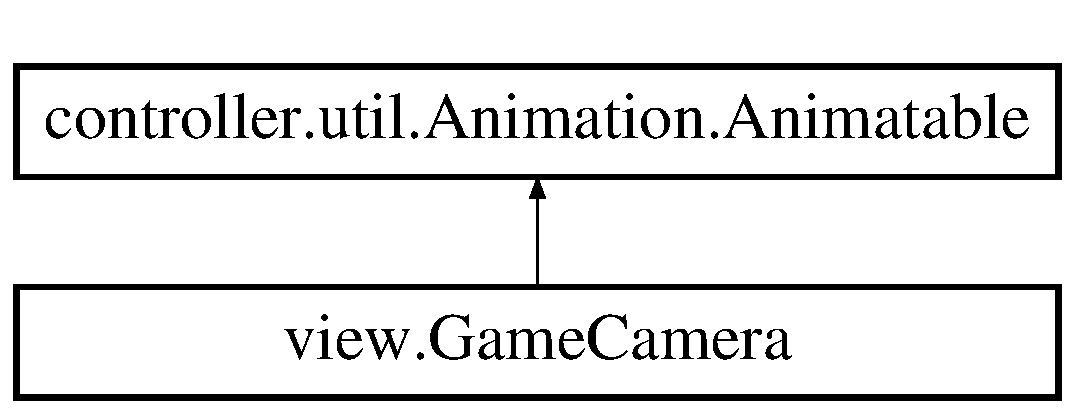
\includegraphics[height=2.000000cm]{classview_1_1_game_camera}
\end{center}
\end{figure}
\subsection*{Public Member Functions}
\begin{DoxyCompactItemize}
\item 
\hypertarget{classview_1_1_game_camera_ab70352e27060caac4c7b4b88a9f75599}{{\bfseries Game\-Camera} (int \-\_\-screen\-Length)}\label{classview_1_1_game_camera_ab70352e27060caac4c7b4b88a9f75599}

\item 
void \hyperlink{classview_1_1_game_camera_adbff38ab55a721adac1eee94d08b341c}{lookat} ()
\item 
Point2\-D.\-Float \hyperlink{classview_1_1_game_camera_afc47415637a247006ca8fb3b4999a671}{get\-Click} (Point2\-D.\-Float point, \hyperlink{classview_1_1_renderer}{Renderer} renderer)
\item 
void \hyperlink{classview_1_1_game_camera_a8ac82709b44bca56a57bdee66491cb73}{set\-Value} (String field\-Name, float value)
\item 
\hypertarget{classview_1_1_game_camera_a760e54d78dea29b1e789ed81941fd0df}{void {\bfseries set\-Screen\-Length} (int length)}\label{classview_1_1_game_camera_a760e54d78dea29b1e789ed81941fd0df}

\item 
\hypertarget{classview_1_1_game_camera_a5d7cfab90132464516798fe70ca062d1}{void {\bfseries set\-Horizontal\-Rotation} (float val)}\label{classview_1_1_game_camera_a5d7cfab90132464516798fe70ca062d1}

\item 
\hypertarget{classview_1_1_game_camera_a19e1f974cccf9607ffc2e9ee5826c8dc}{float {\bfseries get\-Horizontal\-Rotation} ()}\label{classview_1_1_game_camera_a19e1f974cccf9607ffc2e9ee5826c8dc}

\end{DoxyCompactItemize}


\subsection{Detailed Description}
This class represents a camera (or eye) in 3\-D space. The eye is always looking at point 0,0,0 (the center of the board). An the location of the camera is defined in spherical coordinates, where there is a horizontal rotation from \mbox{[}0, 2$\ast$\-P\-I\mbox{]} and a vertical rotation \mbox{[}0, P\-I/2\mbox{]}

\begin{DoxyAuthor}{Author}
Nicholas 
\end{DoxyAuthor}


\subsection{Member Function Documentation}
\hypertarget{classview_1_1_game_camera_afc47415637a247006ca8fb3b4999a671}{\index{view\-::\-Game\-Camera@{view\-::\-Game\-Camera}!get\-Click@{get\-Click}}
\index{get\-Click@{get\-Click}!view::GameCamera@{view\-::\-Game\-Camera}}
\subsubsection[{get\-Click}]{\setlength{\rightskip}{0pt plus 5cm}Point2\-D.\-Float view.\-Game\-Camera.\-get\-Click (
\begin{DoxyParamCaption}
\item[{Point2\-D.\-Float}]{point, }
\item[{{\bf Renderer}}]{renderer}
\end{DoxyParamCaption}
)}}\label{classview_1_1_game_camera_afc47415637a247006ca8fb3b4999a671}
Converts a 2\-D point on the screen to a 3d point that intersects the board (ie the X\-Z plane)


\begin{DoxyParams}{Parameters}
{\em point} & 2\-D point \\
\hline
{\em renderer} & \\
\hline
\end{DoxyParams}
\begin{DoxyReturn}{Returns}
A point whose value represents the x and z intersection at the X\-Z plane 
\end{DoxyReturn}
\hypertarget{classview_1_1_game_camera_adbff38ab55a721adac1eee94d08b341c}{\index{view\-::\-Game\-Camera@{view\-::\-Game\-Camera}!lookat@{lookat}}
\index{lookat@{lookat}!view::GameCamera@{view\-::\-Game\-Camera}}
\subsubsection[{lookat}]{\setlength{\rightskip}{0pt plus 5cm}void view.\-Game\-Camera.\-lookat (
\begin{DoxyParamCaption}
{}
\end{DoxyParamCaption}
)}}\label{classview_1_1_game_camera_adbff38ab55a721adac1eee94d08b341c}
Creates a Model\-View matrix by using the utility method glu\-Look\-At(), supplying the eye location, the look at position(0, 0, 0), and loc.\-x and loc \hypertarget{classview_1_1_game_camera_a8ac82709b44bca56a57bdee66491cb73}{\index{view\-::\-Game\-Camera@{view\-::\-Game\-Camera}!set\-Value@{set\-Value}}
\index{set\-Value@{set\-Value}!view::GameCamera@{view\-::\-Game\-Camera}}
\subsubsection[{set\-Value}]{\setlength{\rightskip}{0pt plus 5cm}void view.\-Game\-Camera.\-set\-Value (
\begin{DoxyParamCaption}
\item[{String}]{field\-Name, }
\item[{float}]{value}
\end{DoxyParamCaption}
)}}\label{classview_1_1_game_camera_a8ac82709b44bca56a57bdee66491cb73}
Method that is called during animation, the camera allows animation around it's horizontal rotation 

Implements \hyperlink{interfacecontroller_1_1util_1_1_animation_1_1_animatable}{controller.\-util.\-Animation.\-Animatable}.



The documentation for this class was generated from the following file\-:\begin{DoxyCompactItemize}
\item 
src/view/Game\-Camera.\-java\end{DoxyCompactItemize}

\hypertarget{classview_1_1_game_frame}{\section{view.\-Game\-Frame Class Reference}
\label{classview_1_1_game_frame}\index{view.\-Game\-Frame@{view.\-Game\-Frame}}
}
Inheritance diagram for view.\-Game\-Frame\-:\begin{figure}[H]
\begin{center}
\leavevmode
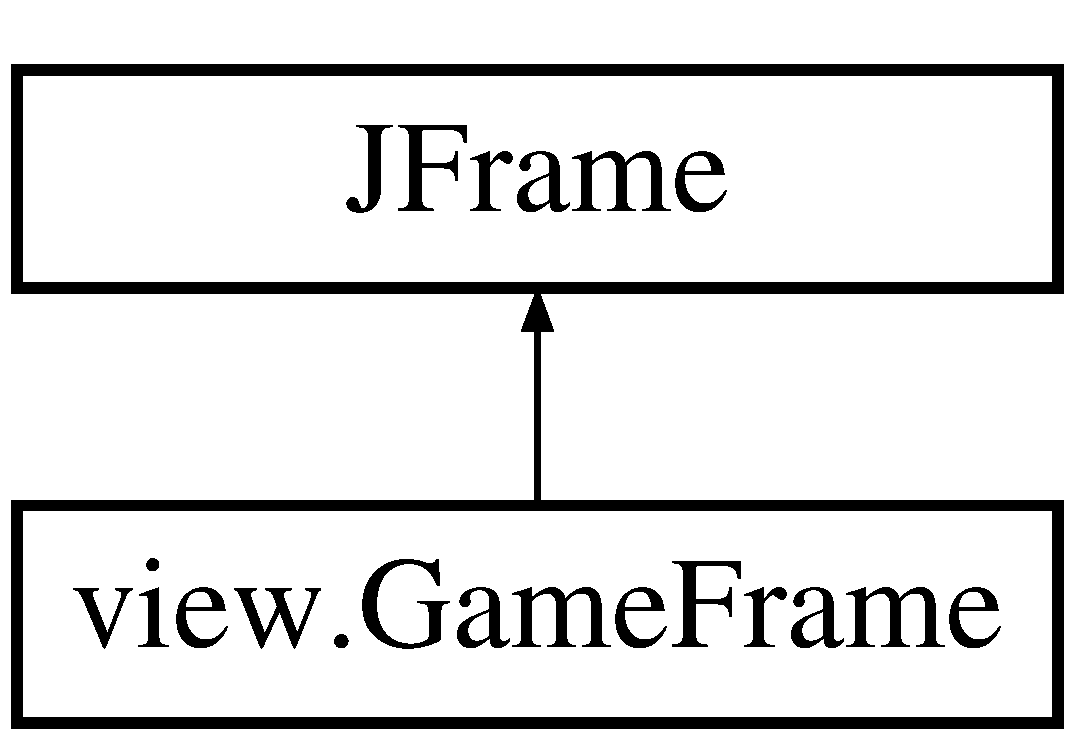
\includegraphics[height=2.000000cm]{classview_1_1_game_frame}
\end{center}
\end{figure}
\subsection*{Public Member Functions}
\begin{DoxyCompactItemize}
\item 
\hypertarget{classview_1_1_game_frame_afbdd0f13c85499fed38a0f83baa4ad0b}{\hyperlink{classcontroller_1_1_game_loop}{Game\-Loop} {\bfseries get\-Game\-Controller} ()}\label{classview_1_1_game_frame_afbdd0f13c85499fed38a0f83baa4ad0b}

\item 
\hypertarget{classview_1_1_game_frame_acd2dd523dbe37ad5b87d9d787b546ed8}{G\-L\-Canvas {\bfseries get\-Canvas} ()}\label{classview_1_1_game_frame_acd2dd523dbe37ad5b87d9d787b546ed8}

\end{DoxyCompactItemize}


\subsection{Detailed Description}
Define a frame for the chess game. This class pieces together all the parts that are needed to make a chess game start, such as the canvas, renderer, input manager, and gameloop. To actually begin the game you must call, get\-Game\-Controller().setup\-New\-Game() with the game mode you wish to play

\begin{DoxyAuthor}{Author}
Nicholas 
\end{DoxyAuthor}


The documentation for this class was generated from the following file\-:\begin{DoxyCompactItemize}
\item 
src/view/Game\-Frame.\-java\end{DoxyCompactItemize}

\hypertarget{classcontroller_1_1_game_loop}{\section{controller.\-Game\-Loop Class Reference}
\label{classcontroller_1_1_game_loop}\index{controller.\-Game\-Loop@{controller.\-Game\-Loop}}
}
Inheritance diagram for controller.\-Game\-Loop\-:\begin{figure}[H]
\begin{center}
\leavevmode
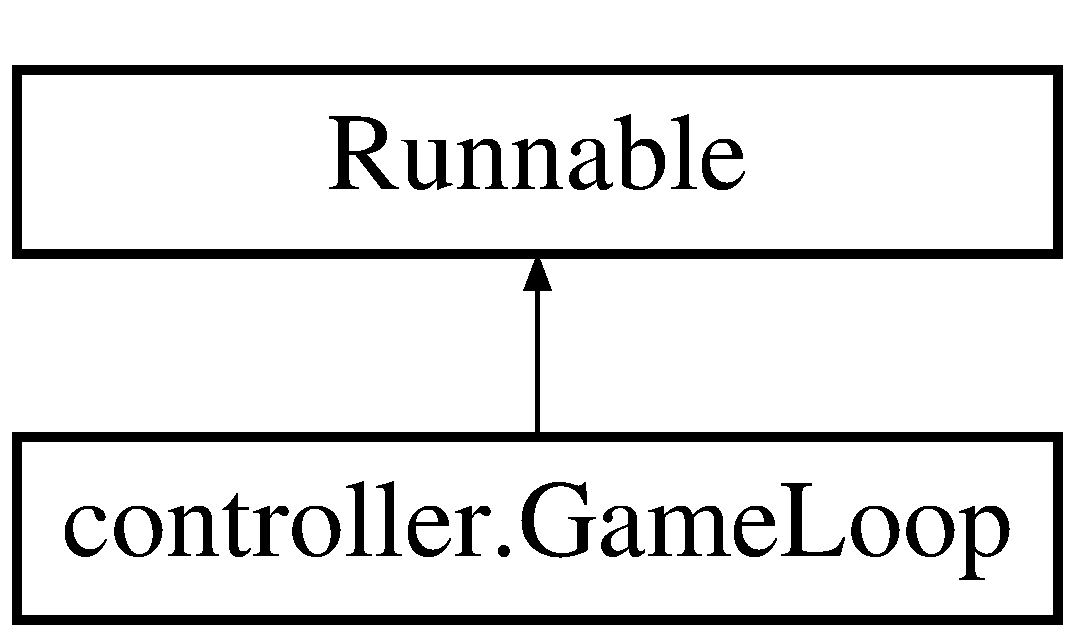
\includegraphics[height=2.000000cm]{classcontroller_1_1_game_loop}
\end{center}
\end{figure}
\subsection*{Public Member Functions}
\begin{DoxyCompactItemize}
\item 
\hyperlink{classcontroller_1_1_game_loop_ad7c4e9e77101658404db3a37b21dfafb}{Game\-Loop} (G\-L\-Canvas \-\_\-canvas, J\-Frame frame)
\item 
synchronized void \hyperlink{classcontroller_1_1_game_loop_a416822fda05ffdbbe385b5157b120a98}{setup\-New\-Game} (\hyperlink{interfacemodel_1_1game__modes_1_1_game_mode}{Game\-Mode} \-\_\-game\-Mode)
\item 
void \hyperlink{classcontroller_1_1_game_loop_a50c1df21b6fcb5de95b90215cc6f0261}{run} ()
\item 
synchronized void \hyperlink{classcontroller_1_1_game_loop_a2f455d14b32197c0506025227b1cfa59}{execute\-Move} (\hyperlink{classmodel_1_1_chess_move}{Chess\-Move} move)
\item 
synchronized void \hyperlink{classcontroller_1_1_game_loop_a9747fb2e4d65a3918d1f589bf6e06e03}{undo\-Last\-Move} ()
\item 
void \hyperlink{classcontroller_1_1_game_loop_a3c58f6ba8b5ec3510ff521c7686e1c11}{cancel\-Game} (\hyperlink{classcontroller_1_1_player}{Player} \-\_\-winner)
\item 
\hypertarget{classcontroller_1_1_game_loop_a8fd38b2b4d1fc537055388bbc369f8e3}{void {\bfseries add\-Animation} (\hyperlink{classcontroller_1_1util_1_1_animation}{Animation} anim)}\label{classcontroller_1_1_game_loop_a8fd38b2b4d1fc537055388bbc369f8e3}

\item 
\hypertarget{classcontroller_1_1_game_loop_a23711cbf256215f376af6854e698c374}{void {\bfseries set\-Renderer} (\hyperlink{classview_1_1_renderer}{Renderer} \-\_\-renderer)}\label{classcontroller_1_1_game_loop_a23711cbf256215f376af6854e698c374}

\item 
\hypertarget{classcontroller_1_1_game_loop_a85488db6ce4c71d17af67eda4f04e3a9}{\hyperlink{classmodel_1_1board_1_1_board}{Board} {\bfseries get\-Board} ()}\label{classcontroller_1_1_game_loop_a85488db6ce4c71d17af67eda4f04e3a9}

\item 
\hypertarget{classcontroller_1_1_game_loop_aa574b3655f4c4c3aa3d04be065a11b2b}{\hyperlink{classcontroller_1_1_player}{Player} {\bfseries get\-Current\-Player} ()}\label{classcontroller_1_1_game_loop_aa574b3655f4c4c3aa3d04be065a11b2b}

\item 
\hypertarget{classcontroller_1_1_game_loop_ac01e3a34770b1b0b92bc55735713c86e}{\hyperlink{classcontroller_1_1_player}{Player} {\bfseries get\-Player1} ()}\label{classcontroller_1_1_game_loop_ac01e3a34770b1b0b92bc55735713c86e}

\item 
\hypertarget{classcontroller_1_1_game_loop_acf6911bb4386ecf2a63ff33fcc21b71c}{\hyperlink{classcontroller_1_1_player}{Player} {\bfseries get\-Player2} ()}\label{classcontroller_1_1_game_loop_acf6911bb4386ecf2a63ff33fcc21b71c}

\item 
\hypertarget{classcontroller_1_1_game_loop_a0dbc7f4a103a2e9447ff109e1e4b12ee}{G\-L\-Canvas {\bfseries get\-Canvas} ()}\label{classcontroller_1_1_game_loop_a0dbc7f4a103a2e9447ff109e1e4b12ee}

\end{DoxyCompactItemize}


\subsection{Detailed Description}
This class will control the gameflow of the program. This class implements the maintaining running loop for this application, and has basic functions that control chess gameflow, such as execute move, cancel game, and setup\-New\-Game

\begin{DoxyAuthor}{Author}
Nicholas 
\end{DoxyAuthor}


\subsection{Constructor \& Destructor Documentation}
\hypertarget{classcontroller_1_1_game_loop_ad7c4e9e77101658404db3a37b21dfafb}{\index{controller\-::\-Game\-Loop@{controller\-::\-Game\-Loop}!Game\-Loop@{Game\-Loop}}
\index{Game\-Loop@{Game\-Loop}!controller::GameLoop@{controller\-::\-Game\-Loop}}
\subsubsection[{Game\-Loop}]{\setlength{\rightskip}{0pt plus 5cm}controller.\-Game\-Loop.\-Game\-Loop (
\begin{DoxyParamCaption}
\item[{G\-L\-Canvas}]{\-\_\-canvas, }
\item[{J\-Frame}]{frame}
\end{DoxyParamCaption}
)}}\label{classcontroller_1_1_game_loop_ad7c4e9e77101658404db3a37b21dfafb}
Constructs a new gameloop, with the given canvas. The renderer is set later.


\begin{DoxyParams}{Parameters}
{\em \-\_\-canvas} & The opengl window created \\
\hline
\end{DoxyParams}


\subsection{Member Function Documentation}
\hypertarget{classcontroller_1_1_game_loop_a3c58f6ba8b5ec3510ff521c7686e1c11}{\index{controller\-::\-Game\-Loop@{controller\-::\-Game\-Loop}!cancel\-Game@{cancel\-Game}}
\index{cancel\-Game@{cancel\-Game}!controller::GameLoop@{controller\-::\-Game\-Loop}}
\subsubsection[{cancel\-Game}]{\setlength{\rightskip}{0pt plus 5cm}void controller.\-Game\-Loop.\-cancel\-Game (
\begin{DoxyParamCaption}
\item[{{\bf Player}}]{\-\_\-winner}
\end{DoxyParamCaption}
)}}\label{classcontroller_1_1_game_loop_a3c58f6ba8b5ec3510ff521c7686e1c11}
Cancels the game, which will result in no moves, being able to be made, but the any animations will finish.


\begin{DoxyParams}{Parameters}
{\em \-\_\-winner} & The winner of the game, can be null in which case the game was a tie \\
\hline
\end{DoxyParams}
\hypertarget{classcontroller_1_1_game_loop_a2f455d14b32197c0506025227b1cfa59}{\index{controller\-::\-Game\-Loop@{controller\-::\-Game\-Loop}!execute\-Move@{execute\-Move}}
\index{execute\-Move@{execute\-Move}!controller::GameLoop@{controller\-::\-Game\-Loop}}
\subsubsection[{execute\-Move}]{\setlength{\rightskip}{0pt plus 5cm}synchronized void controller.\-Game\-Loop.\-execute\-Move (
\begin{DoxyParamCaption}
\item[{{\bf Chess\-Move}}]{move}
\end{DoxyParamCaption}
)}}\label{classcontroller_1_1_game_loop_a2f455d14b32197c0506025227b1cfa59}
Executes a chess move, sets up an animation, and switches the current\-Player. The Chess\-Move is also added the total move list, so it can be undone later if necessary. This move also checks to see if there is any moves left for the other to make, otherwise the game is ended If their is no game running, this method does nothing.


\begin{DoxyParams}{Parameters}
{\em move} & Chess\-Move to be executed, must be a valid\-Move \\
\hline
\end{DoxyParams}
\hypertarget{classcontroller_1_1_game_loop_a50c1df21b6fcb5de95b90215cc6f0261}{\index{controller\-::\-Game\-Loop@{controller\-::\-Game\-Loop}!run@{run}}
\index{run@{run}!controller::GameLoop@{controller\-::\-Game\-Loop}}
\subsubsection[{run}]{\setlength{\rightskip}{0pt plus 5cm}void controller.\-Game\-Loop.\-run (
\begin{DoxyParamCaption}
{}
\end{DoxyParamCaption}
)}}\label{classcontroller_1_1_game_loop_a50c1df21b6fcb5de95b90215cc6f0261}
The method is what runs when start() is called on a thread. The method will continue running until running is set to \char`\"{}false\char`\"{}, ie the game is over. When running is set to false, the winner will be displayed and new game will be set up. \hypertarget{classcontroller_1_1_game_loop_a416822fda05ffdbbe385b5157b120a98}{\index{controller\-::\-Game\-Loop@{controller\-::\-Game\-Loop}!setup\-New\-Game@{setup\-New\-Game}}
\index{setup\-New\-Game@{setup\-New\-Game}!controller::GameLoop@{controller\-::\-Game\-Loop}}
\subsubsection[{setup\-New\-Game}]{\setlength{\rightskip}{0pt plus 5cm}synchronized void controller.\-Game\-Loop.\-setup\-New\-Game (
\begin{DoxyParamCaption}
\item[{{\bf Game\-Mode}}]{\-\_\-game\-Mode}
\end{DoxyParamCaption}
)}}\label{classcontroller_1_1_game_loop_a416822fda05ffdbbe385b5157b120a98}
Sets up the game for the given game\-Mode. This method initializes the players and the board. This method is called automatically, when the current game ends


\begin{DoxyParams}{Parameters}
{\em \-\_\-game\-Mode} & The game mode to be used \\
\hline
\end{DoxyParams}
\hypertarget{classcontroller_1_1_game_loop_a9747fb2e4d65a3918d1f589bf6e06e03}{\index{controller\-::\-Game\-Loop@{controller\-::\-Game\-Loop}!undo\-Last\-Move@{undo\-Last\-Move}}
\index{undo\-Last\-Move@{undo\-Last\-Move}!controller::GameLoop@{controller\-::\-Game\-Loop}}
\subsubsection[{undo\-Last\-Move}]{\setlength{\rightskip}{0pt plus 5cm}synchronized void controller.\-Game\-Loop.\-undo\-Last\-Move (
\begin{DoxyParamCaption}
{}
\end{DoxyParamCaption}
)}}\label{classcontroller_1_1_game_loop_a9747fb2e4d65a3918d1f589bf6e06e03}
Undoes a chess move, sets up an animation, and switches the current\-Player. If their is no game running, or there are moves to undo, this method does nothing.


\begin{DoxyParams}{Parameters}
{\em move} & Chess\-Move to be executed, must be a valid\-Move \\
\hline
\end{DoxyParams}


The documentation for this class was generated from the following file\-:\begin{DoxyCompactItemize}
\item 
src/controller/Game\-Loop.\-java\end{DoxyCompactItemize}

\hypertarget{classview_1_1_game_main_menu}{\section{view.\-Game\-Main\-Menu Class Reference}
\label{classview_1_1_game_main_menu}\index{view.\-Game\-Main\-Menu@{view.\-Game\-Main\-Menu}}
}
Inheritance diagram for view.\-Game\-Main\-Menu\-:\begin{figure}[H]
\begin{center}
\leavevmode
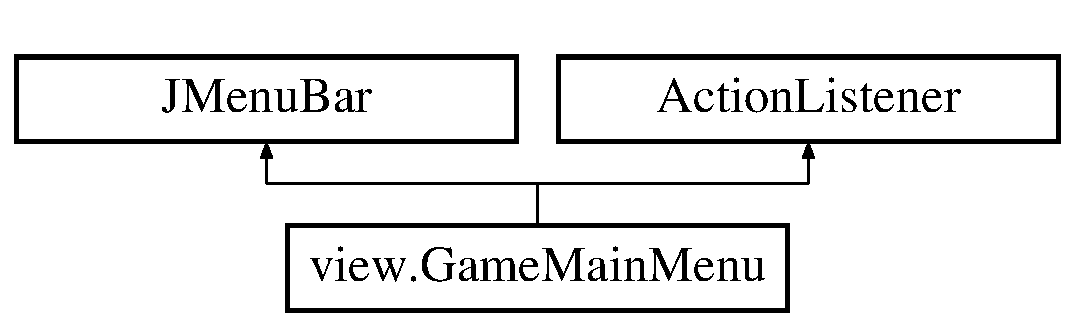
\includegraphics[height=2.000000cm]{classview_1_1_game_main_menu}
\end{center}
\end{figure}
\subsection*{Public Member Functions}
\begin{DoxyCompactItemize}
\item 
\hypertarget{classview_1_1_game_main_menu_a9b03f24e413bbc59660d24f951551068}{{\bfseries Game\-Main\-Menu} (\hyperlink{classview_1_1_game_frame}{Game\-Frame} frame, \hyperlink{classcontroller_1_1_game_loop}{Game\-Loop} controller)}\label{classview_1_1_game_main_menu_a9b03f24e413bbc59660d24f951551068}

\item 
\hypertarget{classview_1_1_game_main_menu_a28cee0ae7e5466223e0e56dc359b00c0}{void {\bfseries action\-Performed} (Action\-Event arg0)}\label{classview_1_1_game_main_menu_a28cee0ae7e5466223e0e56dc359b00c0}

\end{DoxyCompactItemize}


\subsection{Detailed Description}
Menu bar for the Chess game. Contains one drop down menu with 3 options\-: restart, forfeit black, forfeit white. All options trigger a confirm dialog as well.

\begin{DoxyAuthor}{Author}
Nicholas 
\end{DoxyAuthor}


The documentation for this class was generated from the following file\-:\begin{DoxyCompactItemize}
\item 
src/view/Game\-Main\-Menu.\-java\end{DoxyCompactItemize}

\hypertarget{interfacemodel_1_1game__modes_1_1_game_mode}{\section{model.\-game\-\_\-modes.\-Game\-Mode Interface Reference}
\label{interfacemodel_1_1game__modes_1_1_game_mode}\index{model.\-game\-\_\-modes.\-Game\-Mode@{model.\-game\-\_\-modes.\-Game\-Mode}}
}
Inheritance diagram for model.\-game\-\_\-modes.\-Game\-Mode\-:\begin{figure}[H]
\begin{center}
\leavevmode
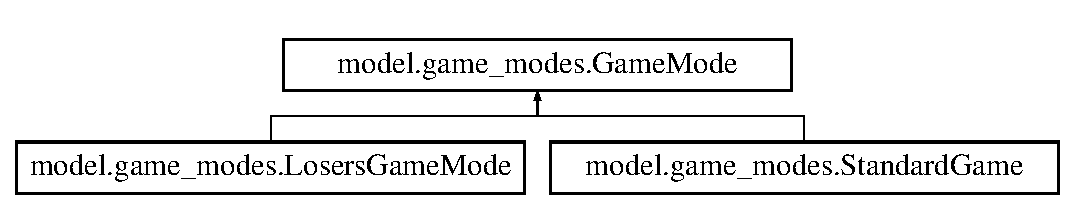
\includegraphics[height=2.000000cm]{interfacemodel_1_1game__modes_1_1_game_mode}
\end{center}
\end{figure}
\subsection*{Public Member Functions}
\begin{DoxyCompactItemize}
\item 
\hyperlink{classmodel_1_1board_1_1_board}{Board} \hyperlink{interfacemodel_1_1game__modes_1_1_game_mode_a237818232e386862838f6b507299497b}{init\-Pieces} (\hyperlink{classcontroller_1_1_player}{Player} player1, \hyperlink{classcontroller_1_1_player}{Player} player2)
\item 
boolean \hyperlink{interfacemodel_1_1game__modes_1_1_game_mode_ab953f82866d9146bde4a2de96af7c308}{board\-Valid} (\hyperlink{classmodel_1_1board_1_1_board}{Board} board, \hyperlink{classcontroller_1_1_player}{Player} victim, \hyperlink{classmodel_1_1_chess_move}{Chess\-Move} last\-Move)
\item 
boolean \hyperlink{interfacemodel_1_1game__modes_1_1_game_mode_adaba2585b6c82e7e14532692db14898f}{has\-Player\-Lost} (\hyperlink{classmodel_1_1board_1_1_board}{Board} board, \hyperlink{classcontroller_1_1_player}{Player} victim)
\item 
void \hyperlink{interfacemodel_1_1game__modes_1_1_game_mode_a034774ac426a436f2c19e7afc8eb8747}{post\-Move\-Action} (final \hyperlink{classcontroller_1_1_game_loop}{Game\-Loop} game\-Controller, \hyperlink{classmodel_1_1_chess_move}{Chess\-Move} last\-Move)
\end{DoxyCompactItemize}


\subsection{Detailed Description}
Provides a basic interface to define a gamemode for a chess game (such as standard, crazyhouse, suicide). These methods are called by the Game\-Loop class.

\begin{DoxyAuthor}{Author}
Nicholas 
\end{DoxyAuthor}


\subsection{Member Function Documentation}
\hypertarget{interfacemodel_1_1game__modes_1_1_game_mode_ab953f82866d9146bde4a2de96af7c308}{\index{model\-::game\-\_\-modes\-::\-Game\-Mode@{model\-::game\-\_\-modes\-::\-Game\-Mode}!board\-Valid@{board\-Valid}}
\index{board\-Valid@{board\-Valid}!model::game_modes::GameMode@{model\-::game\-\_\-modes\-::\-Game\-Mode}}
\subsubsection[{board\-Valid}]{\setlength{\rightskip}{0pt plus 5cm}boolean model.\-game\-\_\-modes.\-Game\-Mode.\-board\-Valid (
\begin{DoxyParamCaption}
\item[{{\bf Board}}]{board, }
\item[{{\bf Player}}]{victim, }
\item[{{\bf Chess\-Move}}]{last\-Move}
\end{DoxyParamCaption}
)}}\label{interfacemodel_1_1game__modes_1_1_game_mode_ab953f82866d9146bde4a2de96af7c308}
Used to determine if a move is \char`\"{}valid\char`\"{} in the context of the \hyperlink{interfacemodel_1_1game__modes_1_1_game_mode}{Game\-Mode}. This method inspects the board and returns true if the board is in a valid state (for a \hyperlink{classmodel_1_1game__modes_1_1_standard_game}{Standard\-Game}, this would check to see if the king is in check)


\begin{DoxyParams}{Parameters}
{\em board} & \\
\hline
{\em victim} & \\
\hline
\end{DoxyParams}
\begin{DoxyReturn}{Returns}
true if the board is in a valid state 
\end{DoxyReturn}


Implemented in \hyperlink{classmodel_1_1game__modes_1_1_standard_game_a532a81128fd4292f85774d2ec383bbe5}{model.\-game\-\_\-modes.\-Standard\-Game}, and \hyperlink{classmodel_1_1game__modes_1_1_losers_game_mode_ab611b89b31571d44240bf530d3944bb0}{model.\-game\-\_\-modes.\-Losers\-Game\-Mode}.

\hypertarget{interfacemodel_1_1game__modes_1_1_game_mode_adaba2585b6c82e7e14532692db14898f}{\index{model\-::game\-\_\-modes\-::\-Game\-Mode@{model\-::game\-\_\-modes\-::\-Game\-Mode}!has\-Player\-Lost@{has\-Player\-Lost}}
\index{has\-Player\-Lost@{has\-Player\-Lost}!model::game_modes::GameMode@{model\-::game\-\_\-modes\-::\-Game\-Mode}}
\subsubsection[{has\-Player\-Lost}]{\setlength{\rightskip}{0pt plus 5cm}boolean model.\-game\-\_\-modes.\-Game\-Mode.\-has\-Player\-Lost (
\begin{DoxyParamCaption}
\item[{{\bf Board}}]{board, }
\item[{{\bf Player}}]{victim}
\end{DoxyParamCaption}
)}}\label{interfacemodel_1_1game__modes_1_1_game_mode_adaba2585b6c82e7e14532692db14898f}
Called when there are no moves left for the current player. At this point the game will be a stalemate or a player has lost.


\begin{DoxyParams}{Parameters}
{\em board} & \\
\hline
{\em victim} & \\
\hline
\end{DoxyParams}
\begin{DoxyReturn}{Returns}
true if the player has lost, false if it is a stalemate 
\end{DoxyReturn}


Implemented in \hyperlink{classmodel_1_1game__modes_1_1_standard_game_af859966b1b11825d30292cc9a6adf3e4}{model.\-game\-\_\-modes.\-Standard\-Game}, and \hyperlink{classmodel_1_1game__modes_1_1_losers_game_mode_a7bd92bacd7df64fff876670d18c7a751}{model.\-game\-\_\-modes.\-Losers\-Game\-Mode}.

\hypertarget{interfacemodel_1_1game__modes_1_1_game_mode_a237818232e386862838f6b507299497b}{\index{model\-::game\-\_\-modes\-::\-Game\-Mode@{model\-::game\-\_\-modes\-::\-Game\-Mode}!init\-Pieces@{init\-Pieces}}
\index{init\-Pieces@{init\-Pieces}!model::game_modes::GameMode@{model\-::game\-\_\-modes\-::\-Game\-Mode}}
\subsubsection[{init\-Pieces}]{\setlength{\rightskip}{0pt plus 5cm}{\bf Board} model.\-game\-\_\-modes.\-Game\-Mode.\-init\-Pieces (
\begin{DoxyParamCaption}
\item[{{\bf Player}}]{player1, }
\item[{{\bf Player}}]{player2}
\end{DoxyParamCaption}
)}}\label{interfacemodel_1_1game__modes_1_1_game_mode_a237818232e386862838f6b507299497b}
Creates a board object with the players passed in. This method will return a complete setup based on the \hyperlink{interfacemodel_1_1game__modes_1_1_game_mode}{Game\-Mode}


\begin{DoxyParams}{Parameters}
{\em player1} & \\
\hline
{\em player2} & \\
\hline
\end{DoxyParams}
\begin{DoxyReturn}{Returns}
Board that has been setup with the rules of the \hyperlink{interfacemodel_1_1game__modes_1_1_game_mode}{Game\-Mode} 
\end{DoxyReturn}


Implemented in \hyperlink{classmodel_1_1game__modes_1_1_standard_game_af204c61bdf19a90aeef707435a65a4b0}{model.\-game\-\_\-modes.\-Standard\-Game}, and \hyperlink{classmodel_1_1game__modes_1_1_losers_game_mode_afe481b52ae8b80ab29365c900b898e8b}{model.\-game\-\_\-modes.\-Losers\-Game\-Mode}.

\hypertarget{interfacemodel_1_1game__modes_1_1_game_mode_a034774ac426a436f2c19e7afc8eb8747}{\index{model\-::game\-\_\-modes\-::\-Game\-Mode@{model\-::game\-\_\-modes\-::\-Game\-Mode}!post\-Move\-Action@{post\-Move\-Action}}
\index{post\-Move\-Action@{post\-Move\-Action}!model::game_modes::GameMode@{model\-::game\-\_\-modes\-::\-Game\-Mode}}
\subsubsection[{post\-Move\-Action}]{\setlength{\rightskip}{0pt plus 5cm}void model.\-game\-\_\-modes.\-Game\-Mode.\-post\-Move\-Action (
\begin{DoxyParamCaption}
\item[{final {\bf Game\-Loop}}]{game\-Controller, }
\item[{{\bf Chess\-Move}}]{last\-Move}
\end{DoxyParamCaption}
)}}\label{interfacemodel_1_1game__modes_1_1_game_mode_a034774ac426a436f2c19e7afc8eb8747}
Called after a move has been executed. This method should display and warning, such as check in a Standard game


\begin{DoxyParams}{Parameters}
{\em game\-Controller} & \\
\hline
{\em last\-Move} & \\
\hline
\end{DoxyParams}


Implemented in \hyperlink{classmodel_1_1game__modes_1_1_standard_game_ac71e444bda1320574ddf4be97724dbb6}{model.\-game\-\_\-modes.\-Standard\-Game}, and \hyperlink{classmodel_1_1game__modes_1_1_losers_game_mode_a489421b50008405e83cde4655e378b81}{model.\-game\-\_\-modes.\-Losers\-Game\-Mode}.



The documentation for this interface was generated from the following file\-:\begin{DoxyCompactItemize}
\item 
src/model/game\-\_\-modes/Game\-Mode.\-java\end{DoxyCompactItemize}

\hypertarget{classcontroller_1_1_input_handler}{\section{controller.\-Input\-Handler Class Reference}
\label{classcontroller_1_1_input_handler}\index{controller.\-Input\-Handler@{controller.\-Input\-Handler}}
}
Inheritance diagram for controller.\-Input\-Handler\-:\begin{figure}[H]
\begin{center}
\leavevmode
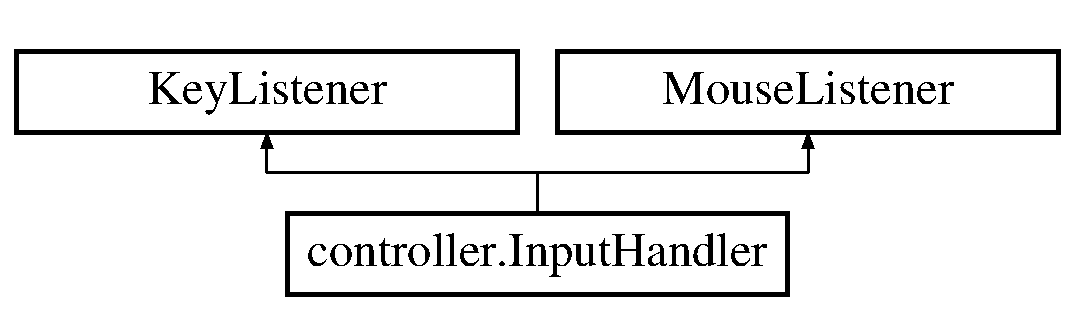
\includegraphics[height=2.000000cm]{classcontroller_1_1_input_handler}
\end{center}
\end{figure}
\subsection*{Public Member Functions}
\begin{DoxyCompactItemize}
\item 
\hypertarget{classcontroller_1_1_input_handler_a892a6081e0cdfcff43180dd3672ef97d}{{\bfseries Input\-Handler} (\hyperlink{classcontroller_1_1_game_loop}{Game\-Loop} \-\_\-game\-Controller, \hyperlink{classview_1_1_renderer}{Renderer} \-\_\-renderer)}\label{classcontroller_1_1_input_handler_a892a6081e0cdfcff43180dd3672ef97d}

\item 
void \hyperlink{classcontroller_1_1_input_handler_a08a9fb76e8c566a168bef8928215c69f}{mouse\-Clicked} (Mouse\-Event arg0)
\item 
\hypertarget{classcontroller_1_1_input_handler_a7f20d015bcca1f8956a48ffca7030204}{void {\bfseries mouse\-Entered} (Mouse\-Event arg0)}\label{classcontroller_1_1_input_handler_a7f20d015bcca1f8956a48ffca7030204}

\item 
\hypertarget{classcontroller_1_1_input_handler_a1afce6568d23b216b51bb660269fbf5b}{void {\bfseries mouse\-Exited} (Mouse\-Event arg0)}\label{classcontroller_1_1_input_handler_a1afce6568d23b216b51bb660269fbf5b}

\item 
\hypertarget{classcontroller_1_1_input_handler_a2f7e2f2634d4c97160800ea684e576d4}{void {\bfseries mouse\-Pressed} (Mouse\-Event arg0)}\label{classcontroller_1_1_input_handler_a2f7e2f2634d4c97160800ea684e576d4}

\item 
\hypertarget{classcontroller_1_1_input_handler_ac32298c58aec32dbdc3aae5a8f5f2ce4}{void {\bfseries mouse\-Released} (Mouse\-Event arg0)}\label{classcontroller_1_1_input_handler_ac32298c58aec32dbdc3aae5a8f5f2ce4}

\item 
void \hyperlink{classcontroller_1_1_input_handler_a744fe9a4f640629b33dca848a74e2eba}{key\-Pressed} (Key\-Event arg0)
\item 
\hypertarget{classcontroller_1_1_input_handler_aae66aefba8d5584b304fda662b508d5b}{void {\bfseries key\-Released} (Key\-Event arg0)}\label{classcontroller_1_1_input_handler_aae66aefba8d5584b304fda662b508d5b}

\item 
\hypertarget{classcontroller_1_1_input_handler_a285eb3a7aaa14fb9946321db3507dcdd}{void {\bfseries key\-Typed} (Key\-Event arg0)}\label{classcontroller_1_1_input_handler_a285eb3a7aaa14fb9946321db3507dcdd}

\end{DoxyCompactItemize}


\subsection{Detailed Description}
Handles any Keystrokes or Mouse-\/clicks that occur within the chess frame. The methods interprets the clicks, and passes along commands to the \hyperlink{classcontroller_1_1_game_loop}{Game\-Loop} or Renderer

\begin{DoxyAuthor}{Author}
Nicholas 
\end{DoxyAuthor}


\subsection{Member Function Documentation}
\hypertarget{classcontroller_1_1_input_handler_a744fe9a4f640629b33dca848a74e2eba}{\index{controller\-::\-Input\-Handler@{controller\-::\-Input\-Handler}!key\-Pressed@{key\-Pressed}}
\index{key\-Pressed@{key\-Pressed}!controller::InputHandler@{controller\-::\-Input\-Handler}}
\subsubsection[{key\-Pressed}]{\setlength{\rightskip}{0pt plus 5cm}void controller.\-Input\-Handler.\-key\-Pressed (
\begin{DoxyParamCaption}
\item[{Key\-Event}]{arg0}
\end{DoxyParamCaption}
)}}\label{classcontroller_1_1_input_handler_a744fe9a4f640629b33dca848a74e2eba}
This method captures any key presses, which currently just handles undo \hypertarget{classcontroller_1_1_input_handler_a08a9fb76e8c566a168bef8928215c69f}{\index{controller\-::\-Input\-Handler@{controller\-::\-Input\-Handler}!mouse\-Clicked@{mouse\-Clicked}}
\index{mouse\-Clicked@{mouse\-Clicked}!controller::InputHandler@{controller\-::\-Input\-Handler}}
\subsubsection[{mouse\-Clicked}]{\setlength{\rightskip}{0pt plus 5cm}void controller.\-Input\-Handler.\-mouse\-Clicked (
\begin{DoxyParamCaption}
\item[{Mouse\-Event}]{arg0}
\end{DoxyParamCaption}
)}}\label{classcontroller_1_1_input_handler_a08a9fb76e8c566a168bef8928215c69f}
This method interprets a click within the chess window. It uses the camera, to find where that click translates into 3\-D space (ie where it intersects the board). This method handles the cases where there is already of selected a piece, and what to do with that piece 

The documentation for this class was generated from the following file\-:\begin{DoxyCompactItemize}
\item 
src/controller/Input\-Handler.\-java\end{DoxyCompactItemize}

\hypertarget{classmodel_1_1pieces_1_1_king}{\section{model.\-pieces.\-King Class Reference}
\label{classmodel_1_1pieces_1_1_king}\index{model.\-pieces.\-King@{model.\-pieces.\-King}}
}
Inheritance diagram for model.\-pieces.\-King\-:\begin{figure}[H]
\begin{center}
\leavevmode
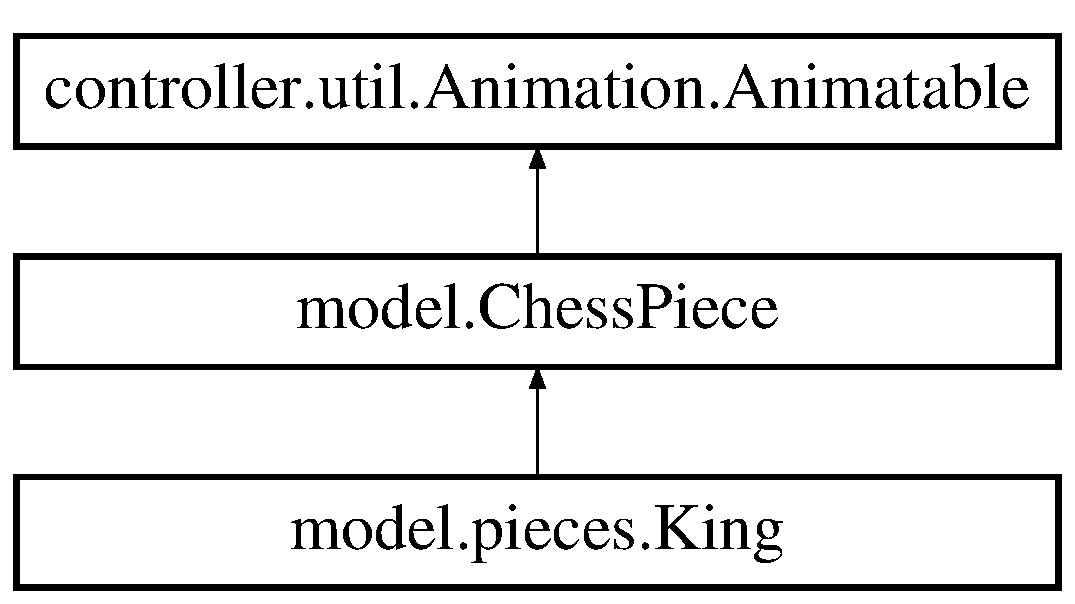
\includegraphics[height=3.000000cm]{classmodel_1_1pieces_1_1_king}
\end{center}
\end{figure}
\subsection*{Public Member Functions}
\begin{DoxyCompactItemize}
\item 
\hypertarget{classmodel_1_1pieces_1_1_king_ab589bb5242906a1fe6f2ccf6db49ff06}{{\bfseries King} (int x, int y, \hyperlink{classmodel_1_1board_1_1_board}{Board} \-\_\-board, \hyperlink{classcontroller_1_1_player}{Player} \-\_\-player)}\label{classmodel_1_1pieces_1_1_king_ab589bb5242906a1fe6f2ccf6db49ff06}

\item 
Array\-List$<$ \hyperlink{classmodel_1_1_chess_move}{Chess\-Move} $>$ \hyperlink{classmodel_1_1pieces_1_1_king_a01079269fe18d60396f980ea099ae7cc}{get\-Possible\-Moves} ()
\item 
String \hyperlink{classmodel_1_1pieces_1_1_king_aae0c46ac679ce113aa2c5bf64997f618}{get\-Type} ()
\end{DoxyCompactItemize}
\subsection*{Additional Inherited Members}


\subsection{Detailed Description}
Represents the \hyperlink{classmodel_1_1pieces_1_1_king}{King}, which in a Standard game results in a loss if captured. Depending on the game a king may not always be important (such as in suicide) so the option to validate check must be passed in, which is used to determine if the king can move into check situation

\begin{DoxyAuthor}{Author}
Nicholas 
\end{DoxyAuthor}


\subsection{Member Function Documentation}
\hypertarget{classmodel_1_1pieces_1_1_king_a01079269fe18d60396f980ea099ae7cc}{\index{model\-::pieces\-::\-King@{model\-::pieces\-::\-King}!get\-Possible\-Moves@{get\-Possible\-Moves}}
\index{get\-Possible\-Moves@{get\-Possible\-Moves}!model::pieces::King@{model\-::pieces\-::\-King}}
\subsubsection[{get\-Possible\-Moves}]{\setlength{\rightskip}{0pt plus 5cm}Array\-List$<${\bf Chess\-Move}$>$ model.\-pieces.\-King.\-get\-Possible\-Moves (
\begin{DoxyParamCaption}
{}
\end{DoxyParamCaption}
)\hspace{0.3cm}{\ttfamily [virtual]}}}\label{classmodel_1_1pieces_1_1_king_a01079269fe18d60396f980ea099ae7cc}
Returns all the diagonal/adjacent moves that the king can capture/move to

N\-O\-T\-E\-: the list of possible moves includes moves that will put this \hyperlink{classmodel_1_1pieces_1_1_king}{King} in check, (if the game allows). This is intentional, if you want a list of valid moves (ie moves that conform the the current Game\-Mode's rules) call \hyperlink{classmodel_1_1_chess_piece_a1f7c0c71547a354d71404b8c8a0020ac}{get\-Valid\-Moves()} 

Implements \hyperlink{classmodel_1_1_chess_piece_a39d690c52727de4a27d2faee4e8b1ac7}{model.\-Chess\-Piece}.

\hypertarget{classmodel_1_1pieces_1_1_king_aae0c46ac679ce113aa2c5bf64997f618}{\index{model\-::pieces\-::\-King@{model\-::pieces\-::\-King}!get\-Type@{get\-Type}}
\index{get\-Type@{get\-Type}!model::pieces::King@{model\-::pieces\-::\-King}}
\subsubsection[{get\-Type}]{\setlength{\rightskip}{0pt plus 5cm}String model.\-pieces.\-King.\-get\-Type (
\begin{DoxyParamCaption}
{}
\end{DoxyParamCaption}
)\hspace{0.3cm}{\ttfamily [virtual]}}}\label{classmodel_1_1pieces_1_1_king_aae0c46ac679ce113aa2c5bf64997f618}
Used to determine a pieces type without using reflection (ie instanceof)

\begin{DoxyReturn}{Returns}
A string that contains the name of the piece, ie the \hyperlink{classmodel_1_1pieces_1_1_pawn}{Pawn} class would return \char`\"{}\-Pawn\char`\"{} 
\end{DoxyReturn}


Implements \hyperlink{classmodel_1_1_chess_piece_a68308e2fa0fe868f7386d40c6cd925df}{model.\-Chess\-Piece}.



The documentation for this class was generated from the following file\-:\begin{DoxyCompactItemize}
\item 
src/model/pieces/King.\-java\end{DoxyCompactItemize}

\hypertarget{classmodel_1_1pieces_1_1_knight}{\section{model.\-pieces.\-Knight Class Reference}
\label{classmodel_1_1pieces_1_1_knight}\index{model.\-pieces.\-Knight@{model.\-pieces.\-Knight}}
}
Inheritance diagram for model.\-pieces.\-Knight\-:\begin{figure}[H]
\begin{center}
\leavevmode
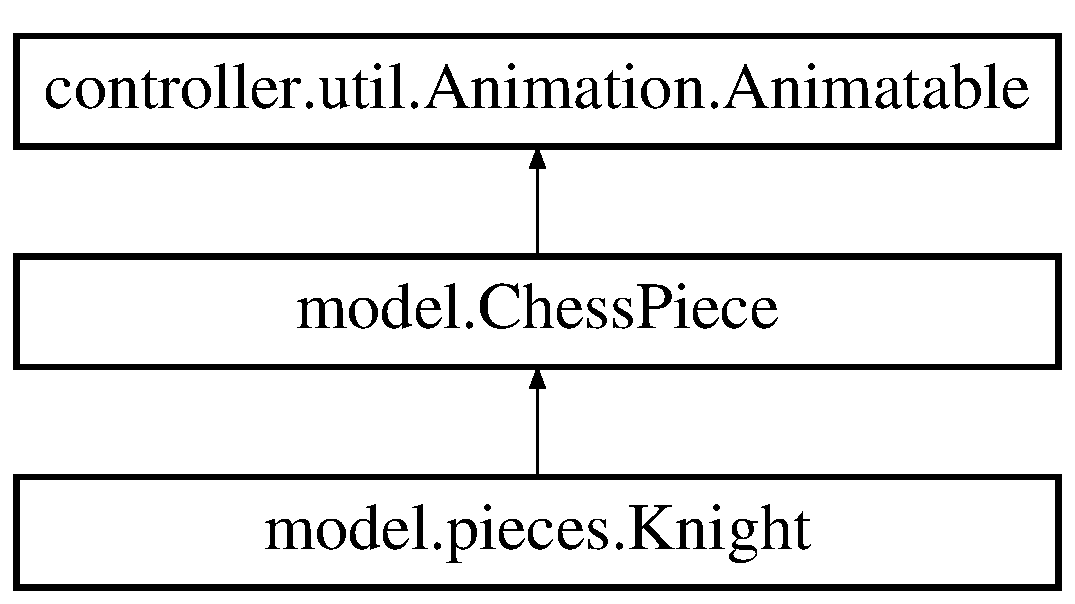
\includegraphics[height=3.000000cm]{classmodel_1_1pieces_1_1_knight}
\end{center}
\end{figure}
\subsection*{Public Member Functions}
\begin{DoxyCompactItemize}
\item 
\hypertarget{classmodel_1_1pieces_1_1_knight_ad3ced5b31e4b389351cf67381dd5949b}{{\bfseries Knight} (int x, int y, \hyperlink{classmodel_1_1board_1_1_board}{Board} \-\_\-board, \hyperlink{classcontroller_1_1_player}{Player} \-\_\-player)}\label{classmodel_1_1pieces_1_1_knight_ad3ced5b31e4b389351cf67381dd5949b}

\item 
Array\-List$<$ \hyperlink{classmodel_1_1_chess_move}{Chess\-Move} $>$ \hyperlink{classmodel_1_1pieces_1_1_knight_a6fc2b0d4bef1c83e84c9351d0b67ae28}{get\-Possible\-Moves} ()
\item 
String \hyperlink{classmodel_1_1pieces_1_1_knight_a692ba3f99660d39fdbfd55c35d709bed}{get\-Type} ()
\end{DoxyCompactItemize}
\subsection*{Additional Inherited Members}


\subsection{Detailed Description}
Represents a \hyperlink{classmodel_1_1pieces_1_1_knight}{Knight}

\begin{DoxyAuthor}{Author}
Nicholas 
\end{DoxyAuthor}


\subsection{Member Function Documentation}
\hypertarget{classmodel_1_1pieces_1_1_knight_a6fc2b0d4bef1c83e84c9351d0b67ae28}{\index{model\-::pieces\-::\-Knight@{model\-::pieces\-::\-Knight}!get\-Possible\-Moves@{get\-Possible\-Moves}}
\index{get\-Possible\-Moves@{get\-Possible\-Moves}!model::pieces::Knight@{model\-::pieces\-::\-Knight}}
\subsubsection[{get\-Possible\-Moves}]{\setlength{\rightskip}{0pt plus 5cm}Array\-List$<${\bf Chess\-Move}$>$ model.\-pieces.\-Knight.\-get\-Possible\-Moves (
\begin{DoxyParamCaption}
{}
\end{DoxyParamCaption}
)\hspace{0.3cm}{\ttfamily [virtual]}}}\label{classmodel_1_1pieces_1_1_knight_a6fc2b0d4bef1c83e84c9351d0b67ae28}
Returns all the moves this knight can make in it's current position 

Implements \hyperlink{classmodel_1_1_chess_piece_a39d690c52727de4a27d2faee4e8b1ac7}{model.\-Chess\-Piece}.

\hypertarget{classmodel_1_1pieces_1_1_knight_a692ba3f99660d39fdbfd55c35d709bed}{\index{model\-::pieces\-::\-Knight@{model\-::pieces\-::\-Knight}!get\-Type@{get\-Type}}
\index{get\-Type@{get\-Type}!model::pieces::Knight@{model\-::pieces\-::\-Knight}}
\subsubsection[{get\-Type}]{\setlength{\rightskip}{0pt plus 5cm}String model.\-pieces.\-Knight.\-get\-Type (
\begin{DoxyParamCaption}
{}
\end{DoxyParamCaption}
)\hspace{0.3cm}{\ttfamily [virtual]}}}\label{classmodel_1_1pieces_1_1_knight_a692ba3f99660d39fdbfd55c35d709bed}
Used to determine a pieces type without using reflection (ie instanceof)

\begin{DoxyReturn}{Returns}
A string that contains the name of the piece, ie the \hyperlink{classmodel_1_1pieces_1_1_pawn}{Pawn} class would return \char`\"{}\-Pawn\char`\"{} 
\end{DoxyReturn}


Implements \hyperlink{classmodel_1_1_chess_piece_a68308e2fa0fe868f7386d40c6cd925df}{model.\-Chess\-Piece}.



The documentation for this class was generated from the following file\-:\begin{DoxyCompactItemize}
\item 
src/model/pieces/Knight.\-java\end{DoxyCompactItemize}

\hypertarget{classmodel_1_1pieces_1_1_lame_queen}{\section{model.\-pieces.\-Lame\-Queen Class Reference}
\label{classmodel_1_1pieces_1_1_lame_queen}\index{model.\-pieces.\-Lame\-Queen@{model.\-pieces.\-Lame\-Queen}}
}
Inheritance diagram for model.\-pieces.\-Lame\-Queen\-:\begin{figure}[H]
\begin{center}
\leavevmode
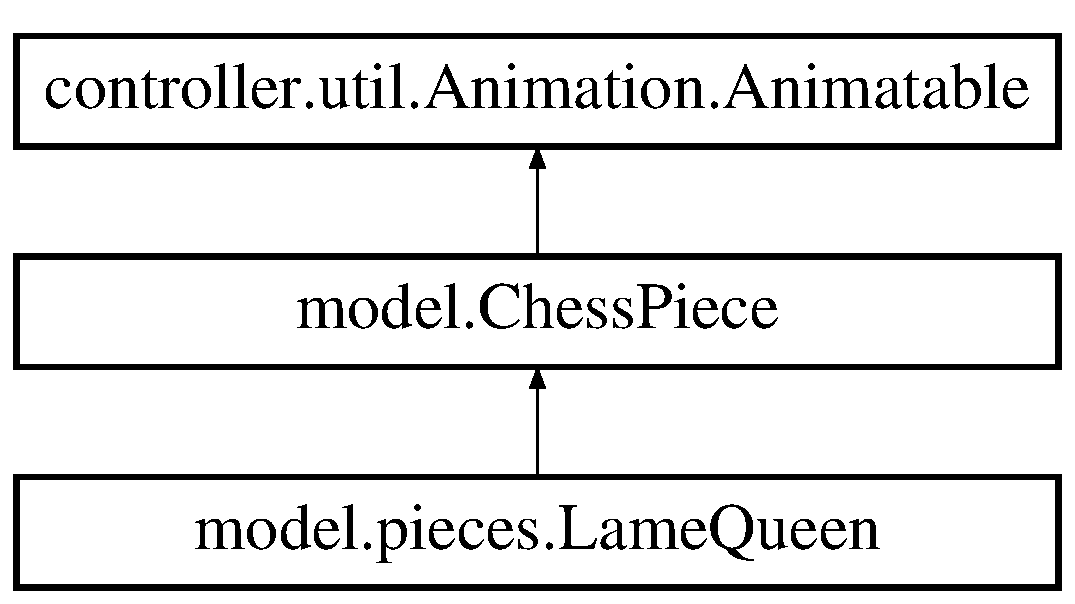
\includegraphics[height=3.000000cm]{classmodel_1_1pieces_1_1_lame_queen}
\end{center}
\end{figure}
\subsection*{Public Member Functions}
\begin{DoxyCompactItemize}
\item 
\hypertarget{classmodel_1_1pieces_1_1_lame_queen_a64065dd218269348eb40c4fc3ddea36c}{{\bfseries Lame\-Queen} (int x, int y, \hyperlink{classmodel_1_1board_1_1_board}{Board} \-\_\-board, \hyperlink{classcontroller_1_1_player}{Player} \-\_\-player)}\label{classmodel_1_1pieces_1_1_lame_queen_a64065dd218269348eb40c4fc3ddea36c}

\item 
Array\-List$<$ \hyperlink{classmodel_1_1_chess_move}{Chess\-Move} $>$ \hyperlink{classmodel_1_1pieces_1_1_lame_queen_a1c58d7e40397c75344909c305f559f7f}{get\-Possible\-Moves} ()
\item 
String \hyperlink{classmodel_1_1pieces_1_1_lame_queen_a70f4bafe5a2b59a281b4ef23f3e3680f}{get\-Type} ()
\end{DoxyCompactItemize}
\subsection*{Additional Inherited Members}


\subsection{Detailed Description}
Represents a \hyperlink{classmodel_1_1pieces_1_1_lame_queen}{Lame\-Queen}. A \hyperlink{classmodel_1_1pieces_1_1_lame_queen}{Lame\-Queen} can move in the same directions as a queen (diagonal and rank-\/file) but can only take pieces on the diagonal.

\begin{DoxyAuthor}{Author}
Nicholas 
\end{DoxyAuthor}


\subsection{Member Function Documentation}
\hypertarget{classmodel_1_1pieces_1_1_lame_queen_a1c58d7e40397c75344909c305f559f7f}{\index{model\-::pieces\-::\-Lame\-Queen@{model\-::pieces\-::\-Lame\-Queen}!get\-Possible\-Moves@{get\-Possible\-Moves}}
\index{get\-Possible\-Moves@{get\-Possible\-Moves}!model::pieces::LameQueen@{model\-::pieces\-::\-Lame\-Queen}}
\subsubsection[{get\-Possible\-Moves}]{\setlength{\rightskip}{0pt plus 5cm}Array\-List$<${\bf Chess\-Move}$>$ model.\-pieces.\-Lame\-Queen.\-get\-Possible\-Moves (
\begin{DoxyParamCaption}
{}
\end{DoxyParamCaption}
)\hspace{0.3cm}{\ttfamily [virtual]}}}\label{classmodel_1_1pieces_1_1_lame_queen_a1c58d7e40397c75344909c305f559f7f}
Returns all the diagonal moves that the \hyperlink{classmodel_1_1pieces_1_1_lame_queen}{Lame\-Queen} can capture/move and the rank-\/file moves that the queen can move 

Implements \hyperlink{classmodel_1_1_chess_piece_a39d690c52727de4a27d2faee4e8b1ac7}{model.\-Chess\-Piece}.

\hypertarget{classmodel_1_1pieces_1_1_lame_queen_a70f4bafe5a2b59a281b4ef23f3e3680f}{\index{model\-::pieces\-::\-Lame\-Queen@{model\-::pieces\-::\-Lame\-Queen}!get\-Type@{get\-Type}}
\index{get\-Type@{get\-Type}!model::pieces::LameQueen@{model\-::pieces\-::\-Lame\-Queen}}
\subsubsection[{get\-Type}]{\setlength{\rightskip}{0pt plus 5cm}String model.\-pieces.\-Lame\-Queen.\-get\-Type (
\begin{DoxyParamCaption}
{}
\end{DoxyParamCaption}
)\hspace{0.3cm}{\ttfamily [virtual]}}}\label{classmodel_1_1pieces_1_1_lame_queen_a70f4bafe5a2b59a281b4ef23f3e3680f}
Used to determine a pieces type without using reflection (ie instanceof)

\begin{DoxyReturn}{Returns}
A string that contains the name of the piece, ie the \hyperlink{classmodel_1_1pieces_1_1_pawn}{Pawn} class would return \char`\"{}\-Pawn\char`\"{} 
\end{DoxyReturn}


Implements \hyperlink{classmodel_1_1_chess_piece_a68308e2fa0fe868f7386d40c6cd925df}{model.\-Chess\-Piece}.



The documentation for this class was generated from the following file\-:\begin{DoxyCompactItemize}
\item 
src/model/pieces/Lame\-Queen.\-java\end{DoxyCompactItemize}

\hypertarget{classmodel_1_1game__modes_1_1_losers_game_mode}{\section{model.\-game\-\_\-modes.\-Losers\-Game\-Mode Class Reference}
\label{classmodel_1_1game__modes_1_1_losers_game_mode}\index{model.\-game\-\_\-modes.\-Losers\-Game\-Mode@{model.\-game\-\_\-modes.\-Losers\-Game\-Mode}}
}
Inheritance diagram for model.\-game\-\_\-modes.\-Losers\-Game\-Mode\-:\begin{figure}[H]
\begin{center}
\leavevmode
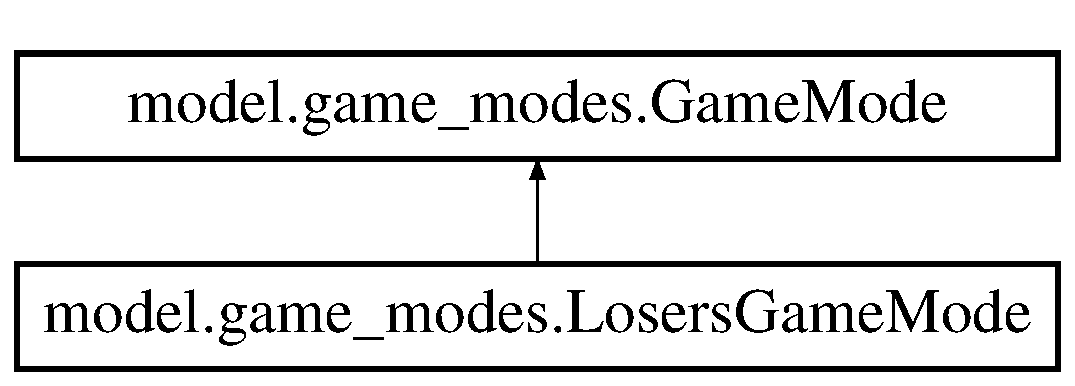
\includegraphics[height=2.000000cm]{classmodel_1_1game__modes_1_1_losers_game_mode}
\end{center}
\end{figure}
\subsection*{Public Member Functions}
\begin{DoxyCompactItemize}
\item 
\hyperlink{classmodel_1_1board_1_1_board}{Board} \hyperlink{classmodel_1_1game__modes_1_1_losers_game_mode_afe481b52ae8b80ab29365c900b898e8b}{init\-Pieces} (\hyperlink{classcontroller_1_1_player}{Player} player1, \hyperlink{classcontroller_1_1_player}{Player} player2)
\item 
boolean \hyperlink{classmodel_1_1game__modes_1_1_losers_game_mode_ab611b89b31571d44240bf530d3944bb0}{board\-Valid} (\hyperlink{classmodel_1_1board_1_1_board}{Board} board, \hyperlink{classcontroller_1_1_player}{Player} victim, \hyperlink{classmodel_1_1_chess_move}{Chess\-Move} last\-Move)
\item 
boolean \hyperlink{classmodel_1_1game__modes_1_1_losers_game_mode_a7bd92bacd7df64fff876670d18c7a751}{has\-Player\-Lost} (\hyperlink{classmodel_1_1board_1_1_board}{Board} board, \hyperlink{classcontroller_1_1_player}{Player} victim)
\item 
void \hyperlink{classmodel_1_1game__modes_1_1_losers_game_mode_a489421b50008405e83cde4655e378b81}{post\-Move\-Action} (final \hyperlink{classcontroller_1_1_game_loop}{Game\-Loop} game\-Controller, \hyperlink{classmodel_1_1_chess_move}{Chess\-Move} last\-Move)
\end{DoxyCompactItemize}


\subsection{Member Function Documentation}
\hypertarget{classmodel_1_1game__modes_1_1_losers_game_mode_ab611b89b31571d44240bf530d3944bb0}{\index{model\-::game\-\_\-modes\-::\-Losers\-Game\-Mode@{model\-::game\-\_\-modes\-::\-Losers\-Game\-Mode}!board\-Valid@{board\-Valid}}
\index{board\-Valid@{board\-Valid}!model::game_modes::LosersGameMode@{model\-::game\-\_\-modes\-::\-Losers\-Game\-Mode}}
\subsubsection[{board\-Valid}]{\setlength{\rightskip}{0pt plus 5cm}boolean model.\-game\-\_\-modes.\-Losers\-Game\-Mode.\-board\-Valid (
\begin{DoxyParamCaption}
\item[{{\bf Board}}]{board, }
\item[{{\bf Player}}]{victim, }
\item[{{\bf Chess\-Move}}]{last\-Move}
\end{DoxyParamCaption}
)}}\label{classmodel_1_1game__modes_1_1_losers_game_mode_ab611b89b31571d44240bf530d3944bb0}
Used to determine if a move is \char`\"{}valid\char`\"{} in the context of the \hyperlink{interfacemodel_1_1game__modes_1_1_game_mode}{Game\-Mode}. This method inspects the board and returns true if the board is in a valid state (for a \hyperlink{classmodel_1_1game__modes_1_1_standard_game}{Standard\-Game}, this would check to see if the king is in check)


\begin{DoxyParams}{Parameters}
{\em board} & \\
\hline
{\em victim} & \\
\hline
\end{DoxyParams}
\begin{DoxyReturn}{Returns}
true if the board is in a valid state 
\end{DoxyReturn}


Implements \hyperlink{interfacemodel_1_1game__modes_1_1_game_mode_ab953f82866d9146bde4a2de96af7c308}{model.\-game\-\_\-modes.\-Game\-Mode}.

\hypertarget{classmodel_1_1game__modes_1_1_losers_game_mode_a7bd92bacd7df64fff876670d18c7a751}{\index{model\-::game\-\_\-modes\-::\-Losers\-Game\-Mode@{model\-::game\-\_\-modes\-::\-Losers\-Game\-Mode}!has\-Player\-Lost@{has\-Player\-Lost}}
\index{has\-Player\-Lost@{has\-Player\-Lost}!model::game_modes::LosersGameMode@{model\-::game\-\_\-modes\-::\-Losers\-Game\-Mode}}
\subsubsection[{has\-Player\-Lost}]{\setlength{\rightskip}{0pt plus 5cm}boolean model.\-game\-\_\-modes.\-Losers\-Game\-Mode.\-has\-Player\-Lost (
\begin{DoxyParamCaption}
\item[{{\bf Board}}]{board, }
\item[{{\bf Player}}]{victim}
\end{DoxyParamCaption}
)}}\label{classmodel_1_1game__modes_1_1_losers_game_mode_a7bd92bacd7df64fff876670d18c7a751}
Called when there are no moves left for the current player. At this point the game will be a stalemate or a player has lost.


\begin{DoxyParams}{Parameters}
{\em board} & \\
\hline
{\em victim} & \\
\hline
\end{DoxyParams}
\begin{DoxyReturn}{Returns}
true if the player has lost, false if it is a stalemate 
\end{DoxyReturn}


Implements \hyperlink{interfacemodel_1_1game__modes_1_1_game_mode_adaba2585b6c82e7e14532692db14898f}{model.\-game\-\_\-modes.\-Game\-Mode}.

\hypertarget{classmodel_1_1game__modes_1_1_losers_game_mode_afe481b52ae8b80ab29365c900b898e8b}{\index{model\-::game\-\_\-modes\-::\-Losers\-Game\-Mode@{model\-::game\-\_\-modes\-::\-Losers\-Game\-Mode}!init\-Pieces@{init\-Pieces}}
\index{init\-Pieces@{init\-Pieces}!model::game_modes::LosersGameMode@{model\-::game\-\_\-modes\-::\-Losers\-Game\-Mode}}
\subsubsection[{init\-Pieces}]{\setlength{\rightskip}{0pt plus 5cm}{\bf Board} model.\-game\-\_\-modes.\-Losers\-Game\-Mode.\-init\-Pieces (
\begin{DoxyParamCaption}
\item[{{\bf Player}}]{player1, }
\item[{{\bf Player}}]{player2}
\end{DoxyParamCaption}
)}}\label{classmodel_1_1game__modes_1_1_losers_game_mode_afe481b52ae8b80ab29365c900b898e8b}
Creates a board object with the players passed in. This method will return a complete setup based on the \hyperlink{interfacemodel_1_1game__modes_1_1_game_mode}{Game\-Mode}


\begin{DoxyParams}{Parameters}
{\em player1} & \\
\hline
{\em player2} & \\
\hline
\end{DoxyParams}
\begin{DoxyReturn}{Returns}
Board that has been setup with the rules of the \hyperlink{interfacemodel_1_1game__modes_1_1_game_mode}{Game\-Mode} 
\end{DoxyReturn}


Implements \hyperlink{interfacemodel_1_1game__modes_1_1_game_mode_a237818232e386862838f6b507299497b}{model.\-game\-\_\-modes.\-Game\-Mode}.

\hypertarget{classmodel_1_1game__modes_1_1_losers_game_mode_a489421b50008405e83cde4655e378b81}{\index{model\-::game\-\_\-modes\-::\-Losers\-Game\-Mode@{model\-::game\-\_\-modes\-::\-Losers\-Game\-Mode}!post\-Move\-Action@{post\-Move\-Action}}
\index{post\-Move\-Action@{post\-Move\-Action}!model::game_modes::LosersGameMode@{model\-::game\-\_\-modes\-::\-Losers\-Game\-Mode}}
\subsubsection[{post\-Move\-Action}]{\setlength{\rightskip}{0pt plus 5cm}void model.\-game\-\_\-modes.\-Losers\-Game\-Mode.\-post\-Move\-Action (
\begin{DoxyParamCaption}
\item[{final {\bf Game\-Loop}}]{game\-Controller, }
\item[{{\bf Chess\-Move}}]{last\-Move}
\end{DoxyParamCaption}
)}}\label{classmodel_1_1game__modes_1_1_losers_game_mode_a489421b50008405e83cde4655e378b81}
Called after a move has been executed. This method should display and warning, such as check in a Standard game


\begin{DoxyParams}{Parameters}
{\em game\-Controller} & \\
\hline
{\em last\-Move} & \\
\hline
\end{DoxyParams}


Implements \hyperlink{interfacemodel_1_1game__modes_1_1_game_mode_a034774ac426a436f2c19e7afc8eb8747}{model.\-game\-\_\-modes.\-Game\-Mode}.



The documentation for this class was generated from the following file\-:\begin{DoxyCompactItemize}
\item 
src/model/game\-\_\-modes/Losers\-Game\-Mode.\-java\end{DoxyCompactItemize}

\hypertarget{classtests_1_1_losers_game_test}{\section{tests.\-Losers\-Game\-Test Class Reference}
\label{classtests_1_1_losers_game_test}\index{tests.\-Losers\-Game\-Test@{tests.\-Losers\-Game\-Test}}
}
\subsection*{Static Public Member Functions}
\begin{DoxyCompactItemize}
\item 
\hypertarget{classtests_1_1_losers_game_test_aedf2329fa598807bd67912d947bc5b3a}{static void {\bfseries main} (String\mbox{[}$\,$\mbox{]} args)}\label{classtests_1_1_losers_game_test_aedf2329fa598807bd67912d947bc5b3a}

\end{DoxyCompactItemize}


The documentation for this class was generated from the following file\-:\begin{DoxyCompactItemize}
\item 
src/tests/Losers\-Game\-Test.\-java\end{DoxyCompactItemize}

\hypertarget{classview_1_1loaders_1_1structures_1_1_model}{\section{view.\-loaders.\-structures.\-Model Class Reference}
\label{classview_1_1loaders_1_1structures_1_1_model}\index{view.\-loaders.\-structures.\-Model@{view.\-loaders.\-structures.\-Model}}
}
\subsection*{Public Member Functions}
\begin{DoxyCompactItemize}
\item 
\hypertarget{classview_1_1loaders_1_1structures_1_1_model_ae6793c35c9c10e2e9d8f3dad712312e8}{{\bfseries Model} (G\-L2 gl, int \-\_\-type, Float\-Buffer \-\_\-buffer, int \-\_\-size, String texture\-Name)}\label{classview_1_1loaders_1_1structures_1_1_model_ae6793c35c9c10e2e9d8f3dad712312e8}

\item 
void \hyperlink{classview_1_1loaders_1_1structures_1_1_model_a15b7163c868eb6450ee4e0f350435b17}{render} (G\-L2 gl)
\end{DoxyCompactItemize}


\subsection{Detailed Description}
This class represents a 3d model, and is responsible for holding a reference to an opengl buffer, and the name of the texture that should be bound before rendering.

\begin{DoxyAuthor}{Author}
Nicholas 
\end{DoxyAuthor}


\subsection{Member Function Documentation}
\hypertarget{classview_1_1loaders_1_1structures_1_1_model_a15b7163c868eb6450ee4e0f350435b17}{\index{view\-::loaders\-::structures\-::\-Model@{view\-::loaders\-::structures\-::\-Model}!render@{render}}
\index{render@{render}!view::loaders::structures::Model@{view\-::loaders\-::structures\-::\-Model}}
\subsubsection[{render}]{\setlength{\rightskip}{0pt plus 5cm}void view.\-loaders.\-structures.\-Model.\-render (
\begin{DoxyParamCaption}
\item[{G\-L2}]{gl}
\end{DoxyParamCaption}
)}}\label{classview_1_1loaders_1_1structures_1_1_model_a15b7163c868eb6450ee4e0f350435b17}
Renders the model. If the vbo has not yet been sent to the G\-P\-U it, will be during the call. Also binds the texture (if specified) associated with this model


\begin{DoxyParams}{Parameters}
{\em gl} & \\
\hline
\end{DoxyParams}


The documentation for this class was generated from the following file\-:\begin{DoxyCompactItemize}
\item 
src/view/loaders/structures/Model.\-java\end{DoxyCompactItemize}

\hypertarget{classmodel_1_1pieces_1_1_pawn}{\section{model.\-pieces.\-Pawn Class Reference}
\label{classmodel_1_1pieces_1_1_pawn}\index{model.\-pieces.\-Pawn@{model.\-pieces.\-Pawn}}
}
Inheritance diagram for model.\-pieces.\-Pawn\-:\begin{figure}[H]
\begin{center}
\leavevmode
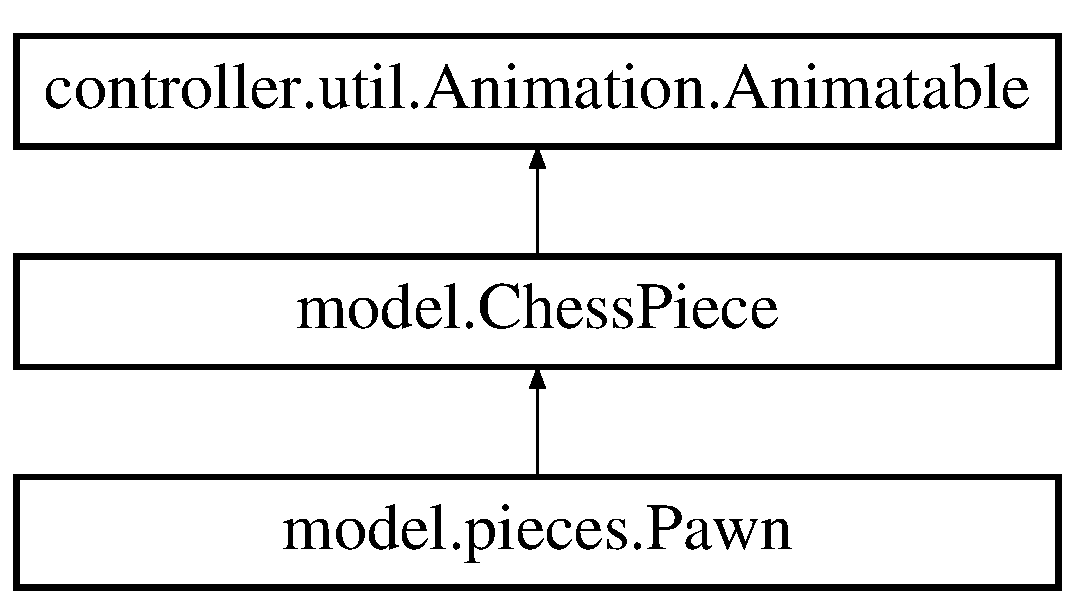
\includegraphics[height=3.000000cm]{classmodel_1_1pieces_1_1_pawn}
\end{center}
\end{figure}
\subsection*{Public Member Functions}
\begin{DoxyCompactItemize}
\item 
\hypertarget{classmodel_1_1pieces_1_1_pawn_a4335d0c4019870c84f05f87cb2e03f0c}{{\bfseries Pawn} (int x, int y, \hyperlink{classmodel_1_1board_1_1_board}{Board} \-\_\-board, \hyperlink{classcontroller_1_1_player}{Player} \-\_\-player)}\label{classmodel_1_1pieces_1_1_pawn_a4335d0c4019870c84f05f87cb2e03f0c}

\item 
Array\-List$<$ \hyperlink{classmodel_1_1_chess_move}{Chess\-Move} $>$ \hyperlink{classmodel_1_1pieces_1_1_pawn_aa8a699402fec460438fe1f9d1ba33632}{get\-Possible\-Moves} ()
\item 
String \hyperlink{classmodel_1_1pieces_1_1_pawn_a3f4abbb3b7e744569928e51f9a7ace27}{get\-Type} ()
\end{DoxyCompactItemize}
\subsection*{Additional Inherited Members}


\subsection{Detailed Description}
Represents a \hyperlink{classmodel_1_1pieces_1_1_pawn}{Pawn}. \hyperlink{classmodel_1_1pieces_1_1_pawn}{Pawn} moving positions are taken directly from the Board object which is responsible for providing the moving directions of a pawn

\begin{DoxyAuthor}{Author}
Nicholas 
\end{DoxyAuthor}


\subsection{Member Function Documentation}
\hypertarget{classmodel_1_1pieces_1_1_pawn_aa8a699402fec460438fe1f9d1ba33632}{\index{model\-::pieces\-::\-Pawn@{model\-::pieces\-::\-Pawn}!get\-Possible\-Moves@{get\-Possible\-Moves}}
\index{get\-Possible\-Moves@{get\-Possible\-Moves}!model::pieces::Pawn@{model\-::pieces\-::\-Pawn}}
\subsubsection[{get\-Possible\-Moves}]{\setlength{\rightskip}{0pt plus 5cm}Array\-List$<${\bf Chess\-Move}$>$ model.\-pieces.\-Pawn.\-get\-Possible\-Moves (
\begin{DoxyParamCaption}
{}
\end{DoxyParamCaption}
)\hspace{0.3cm}{\ttfamily [virtual]}}}\label{classmodel_1_1pieces_1_1_pawn_aa8a699402fec460438fe1f9d1ba33632}
Returns the possible moves this pawn can move. N\-O\-T\-E\-: the class that inherits from board is responsible for checking to see if the pawn has moved. 

Implements \hyperlink{classmodel_1_1_chess_piece_a39d690c52727de4a27d2faee4e8b1ac7}{model.\-Chess\-Piece}.

\hypertarget{classmodel_1_1pieces_1_1_pawn_a3f4abbb3b7e744569928e51f9a7ace27}{\index{model\-::pieces\-::\-Pawn@{model\-::pieces\-::\-Pawn}!get\-Type@{get\-Type}}
\index{get\-Type@{get\-Type}!model::pieces::Pawn@{model\-::pieces\-::\-Pawn}}
\subsubsection[{get\-Type}]{\setlength{\rightskip}{0pt plus 5cm}String model.\-pieces.\-Pawn.\-get\-Type (
\begin{DoxyParamCaption}
{}
\end{DoxyParamCaption}
)\hspace{0.3cm}{\ttfamily [virtual]}}}\label{classmodel_1_1pieces_1_1_pawn_a3f4abbb3b7e744569928e51f9a7ace27}
Used to determine a pieces type without using reflection (ie instanceof)

\begin{DoxyReturn}{Returns}
A string that contains the name of the piece, ie the \hyperlink{classmodel_1_1pieces_1_1_pawn}{Pawn} class would return \char`\"{}\-Pawn\char`\"{} 
\end{DoxyReturn}


Implements \hyperlink{classmodel_1_1_chess_piece_a68308e2fa0fe868f7386d40c6cd925df}{model.\-Chess\-Piece}.



The documentation for this class was generated from the following file\-:\begin{DoxyCompactItemize}
\item 
src/model/pieces/Pawn.\-java\end{DoxyCompactItemize}

\hypertarget{classcontroller_1_1_player}{\section{controller.\-Player Class Reference}
\label{classcontroller_1_1_player}\index{controller.\-Player@{controller.\-Player}}
}
\subsection*{Public Member Functions}
\begin{DoxyCompactItemize}
\item 
\hypertarget{classcontroller_1_1_player_ad6355127f04cc3c7f5462fbe70d0f68b}{{\bfseries Player} (int \-\_\-direction, boolean request\-Name, Component frame)}\label{classcontroller_1_1_player_ad6355127f04cc3c7f5462fbe70d0f68b}

\item 
\hypertarget{classcontroller_1_1_player_ab8a0a1a337ccc52adc53be49c76a88bd}{void {\bfseries reset} ()}\label{classcontroller_1_1_player_ab8a0a1a337ccc52adc53be49c76a88bd}

\item 
void \hyperlink{classcontroller_1_1_player_a518a70950cef524de42c88831baa6c22}{add\-Piece} (\hyperlink{classmodel_1_1_chess_piece}{Chess\-Piece} chess\-Piece)
\item 
\hypertarget{classcontroller_1_1_player_ad119fb7e415d69488a14ebacb27bcd3a}{void {\bfseries piece\-Captured} (\hyperlink{classmodel_1_1_chess_piece}{Chess\-Piece} captured\-Piece)}\label{classcontroller_1_1_player_ad119fb7e415d69488a14ebacb27bcd3a}

\item 
\hypertarget{classcontroller_1_1_player_a3b008486e58dc7deb8bebf8ab803fd99}{void {\bfseries piece\-Uncaptured} (\hyperlink{classmodel_1_1_chess_piece}{Chess\-Piece} uncaptured\-Piece)}\label{classcontroller_1_1_player_a3b008486e58dc7deb8bebf8ab803fd99}

\item 
\hypertarget{classcontroller_1_1_player_ad29800b034a59ef08b14b8ebe7f3f109}{void {\bfseries add\-Win} ()}\label{classcontroller_1_1_player_ad29800b034a59ef08b14b8ebe7f3f109}

\item 
\hypertarget{classcontroller_1_1_player_a7c8b12125102931c40862b340edd51a1}{int {\bfseries get\-Wins} ()}\label{classcontroller_1_1_player_a7c8b12125102931c40862b340edd51a1}

\item 
\hypertarget{classcontroller_1_1_player_a4d1bc127a3148d87b3119247c43ec97d}{Array\-List$<$ \hyperlink{classmodel_1_1_chess_piece}{Chess\-Piece} $>$ {\bfseries get\-Pieces} ()}\label{classcontroller_1_1_player_a4d1bc127a3148d87b3119247c43ec97d}

\item 
\hypertarget{classcontroller_1_1_player_a45539368eae4ca87c67be013487bf530}{\hyperlink{classmodel_1_1pieces_1_1_king}{King} {\bfseries get\-King} ()}\label{classcontroller_1_1_player_a45539368eae4ca87c67be013487bf530}

\item 
\hypertarget{classcontroller_1_1_player_abcbb9063a1c3869c470e35213d7ef4a2}{int {\bfseries get\-Direction} ()}\label{classcontroller_1_1_player_abcbb9063a1c3869c470e35213d7ef4a2}

\item 
\hypertarget{classcontroller_1_1_player_a1ac828358ee773689852e57c8276b041}{float {\bfseries get\-Camera\-Direction} ()}\label{classcontroller_1_1_player_a1ac828358ee773689852e57c8276b041}

\item 
\hypertarget{classcontroller_1_1_player_ac30693c2a47602498b8622dcaf800981}{void {\bfseries set\-Other\-Player} (\hyperlink{classcontroller_1_1_player}{Player} \-\_\-other\-Player)}\label{classcontroller_1_1_player_ac30693c2a47602498b8622dcaf800981}

\item 
\hypertarget{classcontroller_1_1_player_a56768039d96b436827f493324242aaa1}{\hyperlink{classcontroller_1_1_player}{Player} {\bfseries get\-Other\-Player} ()}\label{classcontroller_1_1_player_a56768039d96b436827f493324242aaa1}

\item 
\hypertarget{classcontroller_1_1_player_ad4e558315dda2838b5a1703b5a76c464}{String {\bfseries get\-Player\-Name} ()}\label{classcontroller_1_1_player_ad4e558315dda2838b5a1703b5a76c464}

\item 
\hypertarget{classcontroller_1_1_player_aa7a4928fde7d50da6f6b21d9907a17bb}{String {\bfseries get\-Color\-Texture} ()}\label{classcontroller_1_1_player_aa7a4928fde7d50da6f6b21d9907a17bb}

\end{DoxyCompactItemize}


\subsection{Detailed Description}
\hyperlink{classcontroller_1_1_player}{Player} class responsible for holding it's own chess pieces and the general direction that the pawns travel. The player also holds a reference to the opposing player for easy access.

\begin{DoxyAuthor}{Author}
Nicholas 
\end{DoxyAuthor}


\subsection{Member Function Documentation}
\hypertarget{classcontroller_1_1_player_a518a70950cef524de42c88831baa6c22}{\index{controller\-::\-Player@{controller\-::\-Player}!add\-Piece@{add\-Piece}}
\index{add\-Piece@{add\-Piece}!controller::Player@{controller\-::\-Player}}
\subsubsection[{add\-Piece}]{\setlength{\rightskip}{0pt plus 5cm}void controller.\-Player.\-add\-Piece (
\begin{DoxyParamCaption}
\item[{{\bf Chess\-Piece}}]{chess\-Piece}
\end{DoxyParamCaption}
)}}\label{classcontroller_1_1_player_a518a70950cef524de42c88831baa6c22}
Adds the piece to player, if it is a king store it separately as well to provide easy access


\begin{DoxyParams}{Parameters}
{\em chess\-Piece} & \\
\hline
\end{DoxyParams}


The documentation for this class was generated from the following file\-:\begin{DoxyCompactItemize}
\item 
src/controller/Player.\-java\end{DoxyCompactItemize}

\hypertarget{classmodel_1_1pieces_1_1_queen}{\section{model.\-pieces.\-Queen Class Reference}
\label{classmodel_1_1pieces_1_1_queen}\index{model.\-pieces.\-Queen@{model.\-pieces.\-Queen}}
}
Inheritance diagram for model.\-pieces.\-Queen\-:\begin{figure}[H]
\begin{center}
\leavevmode
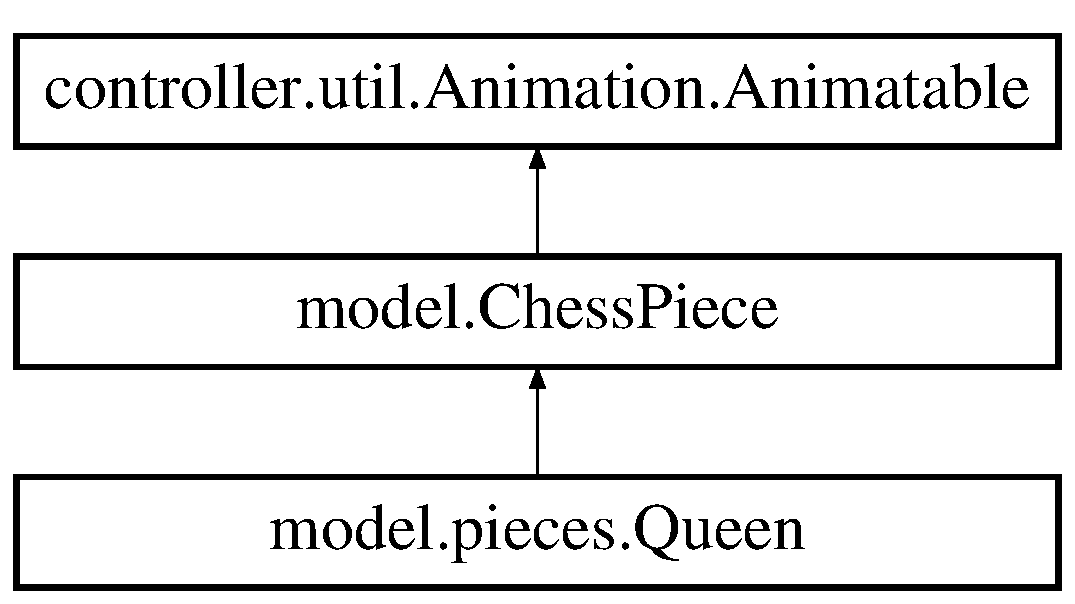
\includegraphics[height=3.000000cm]{classmodel_1_1pieces_1_1_queen}
\end{center}
\end{figure}
\subsection*{Public Member Functions}
\begin{DoxyCompactItemize}
\item 
\hypertarget{classmodel_1_1pieces_1_1_queen_abcce0858220fb4f9d47ee81a15f74adf}{{\bfseries Queen} (int x, int y, \hyperlink{classmodel_1_1board_1_1_board}{Board} \-\_\-board, \hyperlink{classcontroller_1_1_player}{Player} \-\_\-player)}\label{classmodel_1_1pieces_1_1_queen_abcce0858220fb4f9d47ee81a15f74adf}

\item 
Array\-List$<$ \hyperlink{classmodel_1_1_chess_move}{Chess\-Move} $>$ \hyperlink{classmodel_1_1pieces_1_1_queen_a94300f345153c441518363f4bef81f9c}{get\-Possible\-Moves} ()
\item 
String \hyperlink{classmodel_1_1pieces_1_1_queen_acf33a9937af8917615b2a53300830af2}{get\-Type} ()
\end{DoxyCompactItemize}
\subsection*{Additional Inherited Members}


\subsection{Detailed Description}
Represents a \hyperlink{classmodel_1_1pieces_1_1_queen}{Queen}

\begin{DoxyAuthor}{Author}
Nicholas 
\end{DoxyAuthor}


\subsection{Member Function Documentation}
\hypertarget{classmodel_1_1pieces_1_1_queen_a94300f345153c441518363f4bef81f9c}{\index{model\-::pieces\-::\-Queen@{model\-::pieces\-::\-Queen}!get\-Possible\-Moves@{get\-Possible\-Moves}}
\index{get\-Possible\-Moves@{get\-Possible\-Moves}!model::pieces::Queen@{model\-::pieces\-::\-Queen}}
\subsubsection[{get\-Possible\-Moves}]{\setlength{\rightskip}{0pt plus 5cm}Array\-List$<${\bf Chess\-Move}$>$ model.\-pieces.\-Queen.\-get\-Possible\-Moves (
\begin{DoxyParamCaption}
{}
\end{DoxyParamCaption}
)\hspace{0.3cm}{\ttfamily [virtual]}}}\label{classmodel_1_1pieces_1_1_queen_a94300f345153c441518363f4bef81f9c}
Returns all the diagonal and rank-\/file moves that the queen can capture/move 

Implements \hyperlink{classmodel_1_1_chess_piece_a39d690c52727de4a27d2faee4e8b1ac7}{model.\-Chess\-Piece}.

\hypertarget{classmodel_1_1pieces_1_1_queen_acf33a9937af8917615b2a53300830af2}{\index{model\-::pieces\-::\-Queen@{model\-::pieces\-::\-Queen}!get\-Type@{get\-Type}}
\index{get\-Type@{get\-Type}!model::pieces::Queen@{model\-::pieces\-::\-Queen}}
\subsubsection[{get\-Type}]{\setlength{\rightskip}{0pt plus 5cm}String model.\-pieces.\-Queen.\-get\-Type (
\begin{DoxyParamCaption}
{}
\end{DoxyParamCaption}
)\hspace{0.3cm}{\ttfamily [virtual]}}}\label{classmodel_1_1pieces_1_1_queen_acf33a9937af8917615b2a53300830af2}
Used to determine a pieces type without using reflection (ie instanceof)

\begin{DoxyReturn}{Returns}
A string that contains the name of the piece, ie the \hyperlink{classmodel_1_1pieces_1_1_pawn}{Pawn} class would return \char`\"{}\-Pawn\char`\"{} 
\end{DoxyReturn}


Implements \hyperlink{classmodel_1_1_chess_piece_a68308e2fa0fe868f7386d40c6cd925df}{model.\-Chess\-Piece}.



The documentation for this class was generated from the following file\-:\begin{DoxyCompactItemize}
\item 
src/model/pieces/Queen.\-java\end{DoxyCompactItemize}

\hypertarget{classmodel_1_1board_1_1_rectangular_board}{\section{model.\-board.\-Rectangular\-Board Class Reference}
\label{classmodel_1_1board_1_1_rectangular_board}\index{model.\-board.\-Rectangular\-Board@{model.\-board.\-Rectangular\-Board}}
}
Inheritance diagram for model.\-board.\-Rectangular\-Board\-:\begin{figure}[H]
\begin{center}
\leavevmode
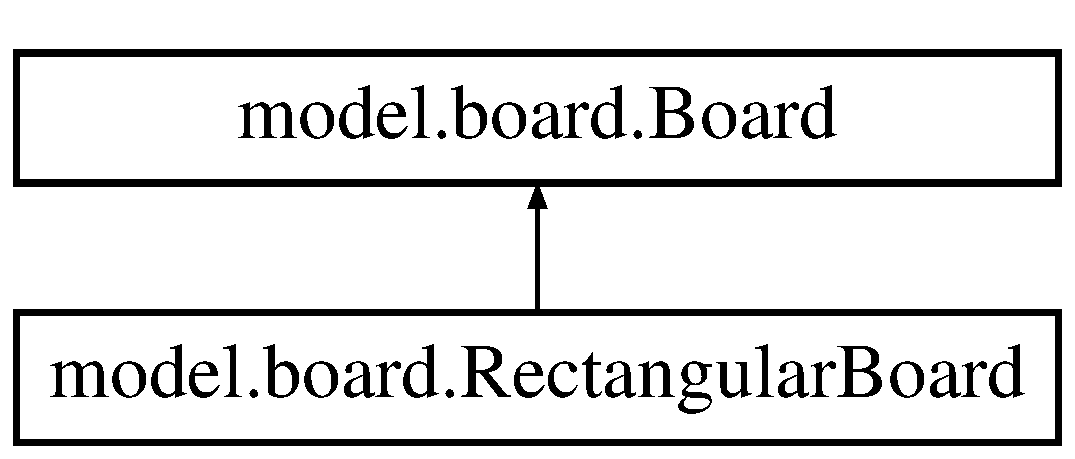
\includegraphics[height=2.000000cm]{classmodel_1_1board_1_1_rectangular_board}
\end{center}
\end{figure}
\subsection*{Public Member Functions}
\begin{DoxyCompactItemize}
\item 
\hyperlink{classmodel_1_1board_1_1_rectangular_board_a9acc529349ad4897e703fd76d86958bc}{Rectangular\-Board} (\hyperlink{interfacemodel_1_1game__modes_1_1_game_mode}{Game\-Mode} \hyperlink{classmodel_1_1board_1_1_board_aeaec4651b92f0416e70eeeaa4959540d}{game\-Mode})
\item 
\hypertarget{classmodel_1_1board_1_1_rectangular_board_ab80e5752c53a80313e2e2ac7372b2022}{{\bfseries Rectangular\-Board} (int \-\_\-width, int \-\_\-length, \hyperlink{interfacemodel_1_1game__modes_1_1_game_mode}{Game\-Mode} \hyperlink{classmodel_1_1board_1_1_board_aeaec4651b92f0416e70eeeaa4959540d}{game\-Mode})}\label{classmodel_1_1board_1_1_rectangular_board_ab80e5752c53a80313e2e2ac7372b2022}

\item 
\hyperlink{classview_1_1loaders_1_1structures_1_1_model}{Model} \hyperlink{classmodel_1_1board_1_1_rectangular_board_a871d89a154bd3628e00504bd91747109}{generate\-Tile\-Model} ()
\item 
\hyperlink{classview_1_1loaders_1_1structures_1_1_model}{Model} \hyperlink{classmodel_1_1board_1_1_rectangular_board_a62edb43eeaeef48c7fd6994806bfc5a4}{generate\-Board\-Model} ()
\item 
String \hyperlink{classmodel_1_1board_1_1_rectangular_board_ae31cbebd45c2e8eb4c0f27a2b31ec290}{get\-Type} ()
\item 
\hyperlink{classmodel_1_1_chess_piece}{Chess\-Piece} \hyperlink{classmodel_1_1board_1_1_rectangular_board_a31120dd8c4e3cb47201a39333945c438}{get\-Tile} (int x, int y)
\item 
\hyperlink{classmodel_1_1_chess_piece}{Chess\-Piece} \hyperlink{classmodel_1_1board_1_1_rectangular_board_a9a77e49749feb9211f8a70e43d12cf4d}{set\-Tile} (\hyperlink{classmodel_1_1_chess_piece}{Chess\-Piece} piece, int x, int y)
\item 
boolean \hyperlink{classmodel_1_1board_1_1_rectangular_board_ac462656a89172957d6970476b4e39bf1}{is\-In\-Bounds} (int x, int y)
\item 
boolean \hyperlink{classmodel_1_1board_1_1_rectangular_board_addce7bd7a463bb3f279df0022ed4a46f}{has\-Enemy\-Piece} (int x, int y, \hyperlink{classcontroller_1_1_player}{Player} player)
\item 
boolean \hyperlink{classmodel_1_1board_1_1_rectangular_board_a4e238edb6b8308d8b561f6418d15e594}{is\-Movable\-Tile} (int x, int y, \hyperlink{classcontroller_1_1_player}{Player} player, boolean can\-Capture)
\item 
Array\-List$<$ Point $>$ \hyperlink{classmodel_1_1board_1_1_rectangular_board_a58a8b1a8a8505340bd2e6dd2f3268aaa}{get\-Adjacent\-Rank\-File\-Tiles} (int x, int y)
\item 
Array\-List$<$ Point $>$ \hyperlink{classmodel_1_1board_1_1_rectangular_board_a43e4180539d99a0b95cf2957b4d43eb2}{get\-Adjacent\-Diagonal\-Tiles} (int x, int y)
\item 
Array\-List$<$ Point $>$ \hyperlink{classmodel_1_1board_1_1_rectangular_board_a32fbc2d65ed36077c051b05d3c305f1f}{get\-Knight\-Moves} (int x, int y)
\item 
Array\-List$<$ Point $>$ \hyperlink{classmodel_1_1board_1_1_rectangular_board_a6323cde6b4f30594520205dfab7fbcba}{get\-Pawn\-Moves} (int x, int y, \hyperlink{classmodel_1_1pieces_1_1_pawn}{Pawn} pawn)
\item 
Array\-List$<$ Point $>$ \hyperlink{classmodel_1_1board_1_1_rectangular_board_a0771a7158bc1c0cbd42c22c95d283f84}{get\-Pawn\-Attacks} (int x, int y, \hyperlink{classmodel_1_1pieces_1_1_pawn}{Pawn} pawn)
\item 
Point \hyperlink{classmodel_1_1board_1_1_rectangular_board_aba36dbe678c51dab2bf11f2735122f4a}{get\-Board\-Position} (Point2\-D.\-Float render\-Point)
\item 
Point2\-D.\-Float \hyperlink{classmodel_1_1board_1_1_rectangular_board_ab566b2108e82dd874969509cbf4ade03}{get\-Render\-Position} (Point loc)
\item 
void \hyperlink{classmodel_1_1board_1_1_rectangular_board_a986119cec9bbcf4699d8c82cd28ede6f}{render} (G\-L2 gl, \hyperlink{classmodel_1_1_chess_piece}{Chess\-Piece} selected\-Piece)
\end{DoxyCompactItemize}
\subsection*{Additional Inherited Members}


\subsection{Detailed Description}
Rectangular board which can be given any dimensions. This class inherits from \hyperlink{classmodel_1_1board_1_1_board}{Board}, and overrides all the methods necessary, using a simple multidimensional array to represent the data. The would be the \hyperlink{classmodel_1_1board_1_1_board}{Board} to use for a standard game of chess (with size (8, 8), or by using the default constructor).

\begin{DoxyAuthor}{Author}
Nicholas 
\end{DoxyAuthor}


\subsection{Constructor \& Destructor Documentation}
\hypertarget{classmodel_1_1board_1_1_rectangular_board_a9acc529349ad4897e703fd76d86958bc}{\index{model\-::board\-::\-Rectangular\-Board@{model\-::board\-::\-Rectangular\-Board}!Rectangular\-Board@{Rectangular\-Board}}
\index{Rectangular\-Board@{Rectangular\-Board}!model::board::RectangularBoard@{model\-::board\-::\-Rectangular\-Board}}
\subsubsection[{Rectangular\-Board}]{\setlength{\rightskip}{0pt plus 5cm}model.\-board.\-Rectangular\-Board.\-Rectangular\-Board (
\begin{DoxyParamCaption}
\item[{{\bf Game\-Mode}}]{game\-Mode}
\end{DoxyParamCaption}
)}}\label{classmodel_1_1board_1_1_rectangular_board_a9acc529349ad4897e703fd76d86958bc}
Constructs a basic board of regulation size (8,8)


\begin{DoxyParams}{Parameters}
{\em game\-Mode} & \\
\hline
\end{DoxyParams}


\subsection{Member Function Documentation}
\hypertarget{classmodel_1_1board_1_1_rectangular_board_a62edb43eeaeef48c7fd6994806bfc5a4}{\index{model\-::board\-::\-Rectangular\-Board@{model\-::board\-::\-Rectangular\-Board}!generate\-Board\-Model@{generate\-Board\-Model}}
\index{generate\-Board\-Model@{generate\-Board\-Model}!model::board::RectangularBoard@{model\-::board\-::\-Rectangular\-Board}}
\subsubsection[{generate\-Board\-Model}]{\setlength{\rightskip}{0pt plus 5cm}{\bf Model} model.\-board.\-Rectangular\-Board.\-generate\-Board\-Model (
\begin{DoxyParamCaption}
{}
\end{DoxyParamCaption}
)\hspace{0.3cm}{\ttfamily [virtual]}}}\label{classmodel_1_1board_1_1_rectangular_board_a62edb43eeaeef48c7fd6994806bfc5a4}
Generates the 3d model for the board, so that it may be added as a model to Asset\-Loader class. N\-O\-T\-E\-: this method is called automatically by the Game\-Loop during setup and should N\-E\-V\-E\-R be called again. The proper way to access this Model would be Asset\-Loader.\-get\-Instace().get\-Model(\hyperlink{classmodel_1_1board_1_1_rectangular_board_ae31cbebd45c2e8eb4c0f27a2b31ec290}{get\-Type()})

\begin{DoxyReturn}{Returns}
the generated board model 
\end{DoxyReturn}


Implements \hyperlink{classmodel_1_1board_1_1_board_a27db942b8b62795b8e8e615c2e39b432}{model.\-board.\-Board}.

\hypertarget{classmodel_1_1board_1_1_rectangular_board_a871d89a154bd3628e00504bd91747109}{\index{model\-::board\-::\-Rectangular\-Board@{model\-::board\-::\-Rectangular\-Board}!generate\-Tile\-Model@{generate\-Tile\-Model}}
\index{generate\-Tile\-Model@{generate\-Tile\-Model}!model::board::RectangularBoard@{model\-::board\-::\-Rectangular\-Board}}
\subsubsection[{generate\-Tile\-Model}]{\setlength{\rightskip}{0pt plus 5cm}{\bf Model} model.\-board.\-Rectangular\-Board.\-generate\-Tile\-Model (
\begin{DoxyParamCaption}
{}
\end{DoxyParamCaption}
)\hspace{0.3cm}{\ttfamily [virtual]}}}\label{classmodel_1_1board_1_1_rectangular_board_a871d89a154bd3628e00504bd91747109}
Generates the 3d model for the board, so that it may be added as a model to Asset\-Loader class. N\-O\-T\-E\-: this method is called automatically by the Game\-Loop during setup and should N\-E\-V\-E\-R be called again. The proper way to access this Model would be Asset\-Loader.\-get\-Instace().get\-Model(\hyperlink{classmodel_1_1board_1_1_rectangular_board_ae31cbebd45c2e8eb4c0f27a2b31ec290}{get\-Type()})

\begin{DoxyReturn}{Returns}
the generated board model 
\end{DoxyReturn}


Implements \hyperlink{classmodel_1_1board_1_1_board_a40de2efe23a2a995394e7223a5c85896}{model.\-board.\-Board}.

\hypertarget{classmodel_1_1board_1_1_rectangular_board_a43e4180539d99a0b95cf2957b4d43eb2}{\index{model\-::board\-::\-Rectangular\-Board@{model\-::board\-::\-Rectangular\-Board}!get\-Adjacent\-Diagonal\-Tiles@{get\-Adjacent\-Diagonal\-Tiles}}
\index{get\-Adjacent\-Diagonal\-Tiles@{get\-Adjacent\-Diagonal\-Tiles}!model::board::RectangularBoard@{model\-::board\-::\-Rectangular\-Board}}
\subsubsection[{get\-Adjacent\-Diagonal\-Tiles}]{\setlength{\rightskip}{0pt plus 5cm}Array\-List$<$Point$>$ model.\-board.\-Rectangular\-Board.\-get\-Adjacent\-Diagonal\-Tiles (
\begin{DoxyParamCaption}
\item[{int}]{x, }
\item[{int}]{y}
\end{DoxyParamCaption}
)\hspace{0.3cm}{\ttfamily [virtual]}}}\label{classmodel_1_1board_1_1_rectangular_board_a43e4180539d99a0b95cf2957b4d43eb2}
Returns 4 spots, (x-\/1, y-\/1), (x-\/1, y+1), (x+1, y-\/1), (x+1, y+1) 

Implements \hyperlink{classmodel_1_1board_1_1_board_a5b3cecdde64a0a00a538fbc69e578f9c}{model.\-board.\-Board}.

\hypertarget{classmodel_1_1board_1_1_rectangular_board_a58a8b1a8a8505340bd2e6dd2f3268aaa}{\index{model\-::board\-::\-Rectangular\-Board@{model\-::board\-::\-Rectangular\-Board}!get\-Adjacent\-Rank\-File\-Tiles@{get\-Adjacent\-Rank\-File\-Tiles}}
\index{get\-Adjacent\-Rank\-File\-Tiles@{get\-Adjacent\-Rank\-File\-Tiles}!model::board::RectangularBoard@{model\-::board\-::\-Rectangular\-Board}}
\subsubsection[{get\-Adjacent\-Rank\-File\-Tiles}]{\setlength{\rightskip}{0pt plus 5cm}Array\-List$<$Point$>$ model.\-board.\-Rectangular\-Board.\-get\-Adjacent\-Rank\-File\-Tiles (
\begin{DoxyParamCaption}
\item[{int}]{x, }
\item[{int}]{y}
\end{DoxyParamCaption}
)\hspace{0.3cm}{\ttfamily [virtual]}}}\label{classmodel_1_1board_1_1_rectangular_board_a58a8b1a8a8505340bd2e6dd2f3268aaa}
Returns 4 spots, (x-\/1, y), (x-\/1, y), (x, y-\/1), (x, y+1) 

Implements \hyperlink{classmodel_1_1board_1_1_board_adae13d194d3acf1ae586162cf8ae6786}{model.\-board.\-Board}.

\hypertarget{classmodel_1_1board_1_1_rectangular_board_aba36dbe678c51dab2bf11f2735122f4a}{\index{model\-::board\-::\-Rectangular\-Board@{model\-::board\-::\-Rectangular\-Board}!get\-Board\-Position@{get\-Board\-Position}}
\index{get\-Board\-Position@{get\-Board\-Position}!model::board::RectangularBoard@{model\-::board\-::\-Rectangular\-Board}}
\subsubsection[{get\-Board\-Position}]{\setlength{\rightskip}{0pt plus 5cm}Point model.\-board.\-Rectangular\-Board.\-get\-Board\-Position (
\begin{DoxyParamCaption}
\item[{Point2\-D.\-Float}]{render\-Point}
\end{DoxyParamCaption}
)\hspace{0.3cm}{\ttfamily [virtual]}}}\label{classmodel_1_1board_1_1_rectangular_board_aba36dbe678c51dab2bf11f2735122f4a}
Converts the given 3d location into a tile location, which can be used to access items on the board


\begin{DoxyParams}{Parameters}
{\em render\-Point} & 3d point \\
\hline
\end{DoxyParams}
\begin{DoxyReturn}{Returns}
tile point representation of loc 
\end{DoxyReturn}


Implements \hyperlink{classmodel_1_1board_1_1_board_adbfd9f6c5999ef5a9705abbfadb8c924}{model.\-board.\-Board}.

\hypertarget{classmodel_1_1board_1_1_rectangular_board_a32fbc2d65ed36077c051b05d3c305f1f}{\index{model\-::board\-::\-Rectangular\-Board@{model\-::board\-::\-Rectangular\-Board}!get\-Knight\-Moves@{get\-Knight\-Moves}}
\index{get\-Knight\-Moves@{get\-Knight\-Moves}!model::board::RectangularBoard@{model\-::board\-::\-Rectangular\-Board}}
\subsubsection[{get\-Knight\-Moves}]{\setlength{\rightskip}{0pt plus 5cm}Array\-List$<$Point$>$ model.\-board.\-Rectangular\-Board.\-get\-Knight\-Moves (
\begin{DoxyParamCaption}
\item[{int}]{x, }
\item[{int}]{y}
\end{DoxyParamCaption}
)\hspace{0.3cm}{\ttfamily [virtual]}}}\label{classmodel_1_1board_1_1_rectangular_board_a32fbc2d65ed36077c051b05d3c305f1f}
Returns 8 spots, all of which form a L shape 

Implements \hyperlink{classmodel_1_1board_1_1_board_ad65a4ec84fc3dad46f5b2f1e97ecc1b0}{model.\-board.\-Board}.

\hypertarget{classmodel_1_1board_1_1_rectangular_board_a0771a7158bc1c0cbd42c22c95d283f84}{\index{model\-::board\-::\-Rectangular\-Board@{model\-::board\-::\-Rectangular\-Board}!get\-Pawn\-Attacks@{get\-Pawn\-Attacks}}
\index{get\-Pawn\-Attacks@{get\-Pawn\-Attacks}!model::board::RectangularBoard@{model\-::board\-::\-Rectangular\-Board}}
\subsubsection[{get\-Pawn\-Attacks}]{\setlength{\rightskip}{0pt plus 5cm}Array\-List$<$Point$>$ model.\-board.\-Rectangular\-Board.\-get\-Pawn\-Attacks (
\begin{DoxyParamCaption}
\item[{int}]{x, }
\item[{int}]{y, }
\item[{{\bf Pawn}}]{pawn}
\end{DoxyParamCaption}
)\hspace{0.3cm}{\ttfamily [virtual]}}}\label{classmodel_1_1board_1_1_rectangular_board_a0771a7158bc1c0cbd42c22c95d283f84}
This method on a rectangular board returns 2 positions, on a rectangular board these are the 2 diagonals in front, while on a hex board they are the top-\/left and top-\/right adjacent tiles.


\begin{DoxyParams}{Parameters}
{\em x} & \hyperlink{classmodel_1_1board_1_1_board}{Board} location x \\
\hline
{\em y} & \hyperlink{classmodel_1_1board_1_1_board}{Board} location y \\
\hline
\end{DoxyParams}
\begin{DoxyReturn}{Returns}
an array of all the positions a pawn at (x, y) can attack on this board 
\end{DoxyReturn}


Implements \hyperlink{classmodel_1_1board_1_1_board_af75b477308f0cb632cf5e164246cd243}{model.\-board.\-Board}.

\hypertarget{classmodel_1_1board_1_1_rectangular_board_a6323cde6b4f30594520205dfab7fbcba}{\index{model\-::board\-::\-Rectangular\-Board@{model\-::board\-::\-Rectangular\-Board}!get\-Pawn\-Moves@{get\-Pawn\-Moves}}
\index{get\-Pawn\-Moves@{get\-Pawn\-Moves}!model::board::RectangularBoard@{model\-::board\-::\-Rectangular\-Board}}
\subsubsection[{get\-Pawn\-Moves}]{\setlength{\rightskip}{0pt plus 5cm}Array\-List$<$Point$>$ model.\-board.\-Rectangular\-Board.\-get\-Pawn\-Moves (
\begin{DoxyParamCaption}
\item[{int}]{x, }
\item[{int}]{y, }
\item[{{\bf Pawn}}]{pawn}
\end{DoxyParamCaption}
)\hspace{0.3cm}{\ttfamily [virtual]}}}\label{classmodel_1_1board_1_1_rectangular_board_a6323cde6b4f30594520205dfab7fbcba}
This method on a rectangular board returns 2 positions if the pawn has not yet moved (the 2 spaces directly in from of the pawn), or 1 move if the pawn has moved The Pawn class is responsible for determining if these locations are valid (ie only one location is valid if it already moved). N\-O\-T\-E\-: these locations may not be in bounds, and must be checked accordingly


\begin{DoxyParams}{Parameters}
{\em x} & \hyperlink{classmodel_1_1board_1_1_board}{Board} location x \\
\hline
{\em y} & \hyperlink{classmodel_1_1board_1_1_board}{Board} location y \\
\hline
\end{DoxyParams}
\begin{DoxyReturn}{Returns}
an array of all the positions a pawn at (x, y) can travel on this board 
\end{DoxyReturn}


Implements \hyperlink{classmodel_1_1board_1_1_board_a4bd4b119f6f5669aaa2aab456056cd92}{model.\-board.\-Board}.

\hypertarget{classmodel_1_1board_1_1_rectangular_board_ab566b2108e82dd874969509cbf4ade03}{\index{model\-::board\-::\-Rectangular\-Board@{model\-::board\-::\-Rectangular\-Board}!get\-Render\-Position@{get\-Render\-Position}}
\index{get\-Render\-Position@{get\-Render\-Position}!model::board::RectangularBoard@{model\-::board\-::\-Rectangular\-Board}}
\subsubsection[{get\-Render\-Position}]{\setlength{\rightskip}{0pt plus 5cm}Point2\-D.\-Float model.\-board.\-Rectangular\-Board.\-get\-Render\-Position (
\begin{DoxyParamCaption}
\item[{Point}]{loc}
\end{DoxyParamCaption}
)\hspace{0.3cm}{\ttfamily [virtual]}}}\label{classmodel_1_1board_1_1_rectangular_board_ab566b2108e82dd874969509cbf4ade03}
Converts the given tile location into 3\-D point, that is scaled to the boards size


\begin{DoxyParams}{Parameters}
{\em loc} & tile location \\
\hline
\end{DoxyParams}
\begin{DoxyReturn}{Returns}
3\-D representation of loc 
\end{DoxyReturn}


Implements \hyperlink{classmodel_1_1board_1_1_board_a2e1be001e288e4501a80844b45024a94}{model.\-board.\-Board}.

\hypertarget{classmodel_1_1board_1_1_rectangular_board_a31120dd8c4e3cb47201a39333945c438}{\index{model\-::board\-::\-Rectangular\-Board@{model\-::board\-::\-Rectangular\-Board}!get\-Tile@{get\-Tile}}
\index{get\-Tile@{get\-Tile}!model::board::RectangularBoard@{model\-::board\-::\-Rectangular\-Board}}
\subsubsection[{get\-Tile}]{\setlength{\rightskip}{0pt plus 5cm}{\bf Chess\-Piece} model.\-board.\-Rectangular\-Board.\-get\-Tile (
\begin{DoxyParamCaption}
\item[{int}]{x, }
\item[{int}]{y}
\end{DoxyParamCaption}
)\hspace{0.3cm}{\ttfamily [virtual]}}}\label{classmodel_1_1board_1_1_rectangular_board_a31120dd8c4e3cb47201a39333945c438}
Returns the piece at the given coordinates, as interpreted by the \hyperlink{classmodel_1_1board_1_1_board}{Board} object.


\begin{DoxyParams}{Parameters}
{\em x} & \\
\hline
{\em y} & \\
\hline
\end{DoxyParams}
\begin{DoxyReturn}{Returns}
the \hyperlink{classmodel_1_1_chess_piece}{Chess\-Piece} at the position, null otherwise 
\end{DoxyReturn}


Implements \hyperlink{classmodel_1_1board_1_1_board_a430d840f3362de265f54f815bf02893a}{model.\-board.\-Board}.

\hypertarget{classmodel_1_1board_1_1_rectangular_board_ae31cbebd45c2e8eb4c0f27a2b31ec290}{\index{model\-::board\-::\-Rectangular\-Board@{model\-::board\-::\-Rectangular\-Board}!get\-Type@{get\-Type}}
\index{get\-Type@{get\-Type}!model::board::RectangularBoard@{model\-::board\-::\-Rectangular\-Board}}
\subsubsection[{get\-Type}]{\setlength{\rightskip}{0pt plus 5cm}String model.\-board.\-Rectangular\-Board.\-get\-Type (
\begin{DoxyParamCaption}
{}
\end{DoxyParamCaption}
)\hspace{0.3cm}{\ttfamily [virtual]}}}\label{classmodel_1_1board_1_1_rectangular_board_ae31cbebd45c2e8eb4c0f27a2b31ec290}
String used to identify the type of board. Also used as a unique model name

\begin{DoxyReturn}{Returns}
String used to identify the type of board 
\end{DoxyReturn}


Implements \hyperlink{classmodel_1_1board_1_1_board_a6d5675d9156c70de1c08842cea728749}{model.\-board.\-Board}.

\hypertarget{classmodel_1_1board_1_1_rectangular_board_addce7bd7a463bb3f279df0022ed4a46f}{\index{model\-::board\-::\-Rectangular\-Board@{model\-::board\-::\-Rectangular\-Board}!has\-Enemy\-Piece@{has\-Enemy\-Piece}}
\index{has\-Enemy\-Piece@{has\-Enemy\-Piece}!model::board::RectangularBoard@{model\-::board\-::\-Rectangular\-Board}}
\subsubsection[{has\-Enemy\-Piece}]{\setlength{\rightskip}{0pt plus 5cm}boolean model.\-board.\-Rectangular\-Board.\-has\-Enemy\-Piece (
\begin{DoxyParamCaption}
\item[{int}]{x, }
\item[{int}]{y, }
\item[{{\bf Player}}]{attacker}
\end{DoxyParamCaption}
)\hspace{0.3cm}{\ttfamily [virtual]}}}\label{classmodel_1_1board_1_1_rectangular_board_addce7bd7a463bb3f279df0022ed4a46f}

\begin{DoxyParams}{Parameters}
{\em x} & \hyperlink{classmodel_1_1board_1_1_board}{Board} location x \\
\hline
{\em y} & \hyperlink{classmodel_1_1board_1_1_board}{Board} location y \\
\hline
{\em attacker} & The player making the move \\
\hline
\end{DoxyParams}
\begin{DoxyReturn}{Returns}
true if the tile at (x, y) contains a piece of the opposing player 
\end{DoxyReturn}


Implements \hyperlink{classmodel_1_1board_1_1_board_ae6c8e172c9bb977b3be9f023736a3f80}{model.\-board.\-Board}.

\hypertarget{classmodel_1_1board_1_1_rectangular_board_ac462656a89172957d6970476b4e39bf1}{\index{model\-::board\-::\-Rectangular\-Board@{model\-::board\-::\-Rectangular\-Board}!is\-In\-Bounds@{is\-In\-Bounds}}
\index{is\-In\-Bounds@{is\-In\-Bounds}!model::board::RectangularBoard@{model\-::board\-::\-Rectangular\-Board}}
\subsubsection[{is\-In\-Bounds}]{\setlength{\rightskip}{0pt plus 5cm}boolean model.\-board.\-Rectangular\-Board.\-is\-In\-Bounds (
\begin{DoxyParamCaption}
\item[{int}]{x, }
\item[{int}]{y}
\end{DoxyParamCaption}
)\hspace{0.3cm}{\ttfamily [virtual]}}}\label{classmodel_1_1board_1_1_rectangular_board_ac462656a89172957d6970476b4e39bf1}

\begin{DoxyParams}{Parameters}
{\em x} & \hyperlink{classmodel_1_1board_1_1_board}{Board} location x \\
\hline
{\em y} & \hyperlink{classmodel_1_1board_1_1_board}{Board} location y \\
\hline
\end{DoxyParams}
\begin{DoxyReturn}{Returns}
true if the given location is within the boards dimensions, false otherwise 
\end{DoxyReturn}


Implements \hyperlink{classmodel_1_1board_1_1_board_a7c4c6d14284584b90dd969ba80bda496}{model.\-board.\-Board}.

\hypertarget{classmodel_1_1board_1_1_rectangular_board_a4e238edb6b8308d8b561f6418d15e594}{\index{model\-::board\-::\-Rectangular\-Board@{model\-::board\-::\-Rectangular\-Board}!is\-Movable\-Tile@{is\-Movable\-Tile}}
\index{is\-Movable\-Tile@{is\-Movable\-Tile}!model::board::RectangularBoard@{model\-::board\-::\-Rectangular\-Board}}
\subsubsection[{is\-Movable\-Tile}]{\setlength{\rightskip}{0pt plus 5cm}boolean model.\-board.\-Rectangular\-Board.\-is\-Movable\-Tile (
\begin{DoxyParamCaption}
\item[{int}]{x, }
\item[{int}]{y, }
\item[{{\bf Player}}]{attacker, }
\item[{boolean}]{can\-Capture}
\end{DoxyParamCaption}
)\hspace{0.3cm}{\ttfamily [virtual]}}}\label{classmodel_1_1board_1_1_rectangular_board_a4e238edb6b8308d8b561f6418d15e594}

\begin{DoxyParams}{Parameters}
{\em x} & \hyperlink{classmodel_1_1board_1_1_board}{Board} location x \\
\hline
{\em y} & \hyperlink{classmodel_1_1board_1_1_board}{Board} location y \\
\hline
{\em attacker} & The player making the move \\
\hline
{\em can\-Capture} & If a piece is able to capture on the the tile \\
\hline
\end{DoxyParams}
\begin{DoxyReturn}{Returns}
true if the space is open (ie no piece is on the tile) or if the tile contains an enemy piece, and the attacker can capture it 
\end{DoxyReturn}


Implements \hyperlink{classmodel_1_1board_1_1_board_abbfd0ab523b5a8953556ff6aad8d42c6}{model.\-board.\-Board}.

\hypertarget{classmodel_1_1board_1_1_rectangular_board_a986119cec9bbcf4699d8c82cd28ede6f}{\index{model\-::board\-::\-Rectangular\-Board@{model\-::board\-::\-Rectangular\-Board}!render@{render}}
\index{render@{render}!model::board::RectangularBoard@{model\-::board\-::\-Rectangular\-Board}}
\subsubsection[{render}]{\setlength{\rightskip}{0pt plus 5cm}void model.\-board.\-Rectangular\-Board.\-render (
\begin{DoxyParamCaption}
\item[{G\-L2}]{gl, }
\item[{{\bf Chess\-Piece}}]{selected\-Piece}
\end{DoxyParamCaption}
)\hspace{0.3cm}{\ttfamily [virtual]}}}\label{classmodel_1_1board_1_1_rectangular_board_a986119cec9bbcf4699d8c82cd28ede6f}
Renders the board with the given opengl context. This methods renders the board's mesh, and all the pieces on the board, by repeated calls to Chess\-Piece.\-render(gl);


\begin{DoxyParams}{Parameters}
{\em gl} & \\
\hline
{\em selected\-Piece} & \\
\hline
\end{DoxyParams}


Implements \hyperlink{classmodel_1_1board_1_1_board_a2680e928007fbd344f4640e053861883}{model.\-board.\-Board}.

\hypertarget{classmodel_1_1board_1_1_rectangular_board_a9a77e49749feb9211f8a70e43d12cf4d}{\index{model\-::board\-::\-Rectangular\-Board@{model\-::board\-::\-Rectangular\-Board}!set\-Tile@{set\-Tile}}
\index{set\-Tile@{set\-Tile}!model::board::RectangularBoard@{model\-::board\-::\-Rectangular\-Board}}
\subsubsection[{set\-Tile}]{\setlength{\rightskip}{0pt plus 5cm}{\bf Chess\-Piece} model.\-board.\-Rectangular\-Board.\-set\-Tile (
\begin{DoxyParamCaption}
\item[{{\bf Chess\-Piece}}]{piece, }
\item[{int}]{x, }
\item[{int}]{y}
\end{DoxyParamCaption}
)\hspace{0.3cm}{\ttfamily [virtual]}}}\label{classmodel_1_1board_1_1_rectangular_board_a9a77e49749feb9211f8a70e43d12cf4d}
Sets the piece to the (x, y) position, and sets the internal board\-Location of the piece. If a piece already existed it is removed from the board, location set to (-\/1, -\/1) and returned


\begin{DoxyParams}{Parameters}
{\em piece} & Piece to be moved \\
\hline
{\em x} & \hyperlink{classmodel_1_1board_1_1_board}{Board} location x \\
\hline
{\em y} & \hyperlink{classmodel_1_1board_1_1_board}{Board} location y \\
\hline
\end{DoxyParams}
\begin{DoxyReturn}{Returns}
the piece that was occupying this tile, null otherwise 
\end{DoxyReturn}


Implements \hyperlink{classmodel_1_1board_1_1_board_a2ee2df58c449ad4251b26266a1c326d7}{model.\-board.\-Board}.



The documentation for this class was generated from the following file\-:\begin{DoxyCompactItemize}
\item 
src/model/board/Rectangular\-Board.\-java\end{DoxyCompactItemize}

\hypertarget{classview_1_1_renderer}{\section{view.\-Renderer Class Reference}
\label{classview_1_1_renderer}\index{view.\-Renderer@{view.\-Renderer}}
}
Inheritance diagram for view.\-Renderer\-:\begin{figure}[H]
\begin{center}
\leavevmode
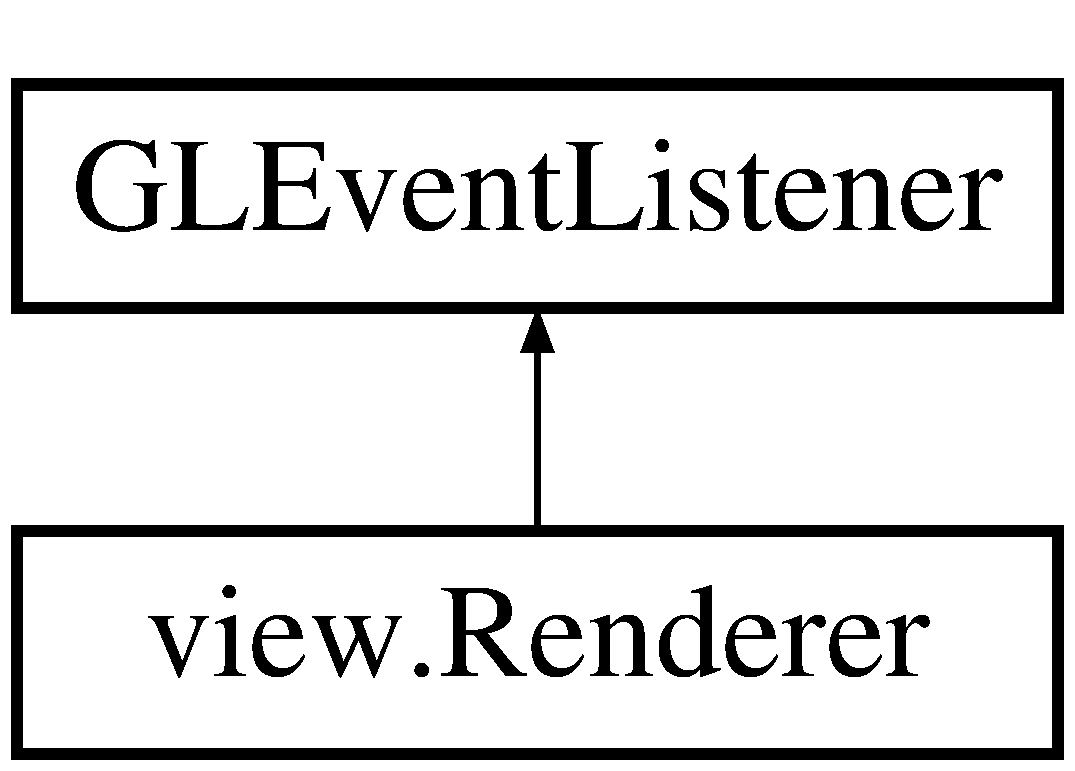
\includegraphics[height=2.000000cm]{classview_1_1_renderer}
\end{center}
\end{figure}
\subsection*{Public Member Functions}
\begin{DoxyCompactItemize}
\item 
\hypertarget{classview_1_1_renderer_af97a8eb943cc205b1a1ea934c3e78776}{{\bfseries Renderer} (\hyperlink{classcontroller_1_1_game_loop}{Game\-Loop} \-\_\-game\-Controller)}\label{classview_1_1_renderer_af97a8eb943cc205b1a1ea934c3e78776}

\item 
void \hyperlink{classview_1_1_renderer_a735a52a16cb1a2c7b21b0b47e140bccc}{display} (G\-L\-Auto\-Drawable g\-L\-Drawable)
\item 
\hypertarget{classview_1_1_renderer_a83b1d62f674e3b265dd7f1265b93456d}{void {\bfseries dispose} (G\-L\-Auto\-Drawable arg0)}\label{classview_1_1_renderer_a83b1d62f674e3b265dd7f1265b93456d}

\item 
void \hyperlink{classview_1_1_renderer_a8cc3379eb90aa67965f780ec5d93b95a}{init} (G\-L\-Auto\-Drawable g\-L\-Drawable)
\item 
\hypertarget{classview_1_1_renderer_a21dae4f98ad6665bbd93318f295cb0d7}{void {\bfseries reshape} (G\-L\-Auto\-Drawable g\-L\-Drawable, int x, int y, int width, int height)}\label{classview_1_1_renderer_a21dae4f98ad6665bbd93318f295cb0d7}

\item 
\hypertarget{classview_1_1_renderer_a538710e08ee1d46f7f25f4ecc8d2f034}{void {\bfseries set\-Selected\-Piece} (\hyperlink{classmodel_1_1_chess_piece}{Chess\-Piece} piece)}\label{classview_1_1_renderer_a538710e08ee1d46f7f25f4ecc8d2f034}

\item 
\hypertarget{classview_1_1_renderer_ac5de3cf59a0aa541a7b46c4c3bbab477}{\hyperlink{classmodel_1_1_chess_piece}{Chess\-Piece} {\bfseries get\-Selected\-Piece} ()}\label{classview_1_1_renderer_ac5de3cf59a0aa541a7b46c4c3bbab477}

\item 
\hypertarget{classview_1_1_renderer_a92f219c1d810a39003a9480594978cad}{\hyperlink{classview_1_1_game_camera}{Game\-Camera} {\bfseries get\-Camera} ()}\label{classview_1_1_renderer_a92f219c1d810a39003a9480594978cad}

\item 
\hypertarget{classview_1_1_renderer_ab38191d5cd62c4bfc8da1ffa4403b993}{float\mbox{[}$\,$\mbox{]} {\bfseries get\-Model\-View\-Matrix} ()}\label{classview_1_1_renderer_ab38191d5cd62c4bfc8da1ffa4403b993}

\item 
\hypertarget{classview_1_1_renderer_ac7725d68a5f929a47cb6b70a747a42ed}{float\mbox{[}$\,$\mbox{]} {\bfseries get\-Projection\-Matrix} ()}\label{classview_1_1_renderer_ac7725d68a5f929a47cb6b70a747a42ed}

\item 
\hypertarget{classview_1_1_renderer_a5f18309c0140551d21ac5477c68a8db0}{int\mbox{[}$\,$\mbox{]} {\bfseries get\-Viewport\-Dimensions} ()}\label{classview_1_1_renderer_a5f18309c0140551d21ac5477c68a8db0}

\item 
\hypertarget{classview_1_1_renderer_a5201eddadd61f8f8fd013031fd6c5e75}{synchronized boolean {\bfseries is\-Initilized} ()}\label{classview_1_1_renderer_a5201eddadd61f8f8fd013031fd6c5e75}

\end{DoxyCompactItemize}


\subsection{Detailed Description}
The Render class implements the functionality of a G\-L\-Event\-Listener which defines the methods that are called by the underlying G\-L\-Canvas. Upon create of the G\-L\-Canvas, the G\-L\-Canvas calls \hyperlink{classview_1_1_renderer_a8cc3379eb90aa67965f780ec5d93b95a}{init()}, reshape(), then \hyperlink{classview_1_1_renderer_a735a52a16cb1a2c7b21b0b47e140bccc}{display()}, which are each defined here. Any calls to repaint window, will eventually lead to a \hyperlink{classview_1_1_renderer_a735a52a16cb1a2c7b21b0b47e140bccc}{display()} call defined here

\begin{DoxyAuthor}{Author}
Nicholas 
\end{DoxyAuthor}


\subsection{Member Function Documentation}
\hypertarget{classview_1_1_renderer_a735a52a16cb1a2c7b21b0b47e140bccc}{\index{view\-::\-Renderer@{view\-::\-Renderer}!display@{display}}
\index{display@{display}!view::Renderer@{view\-::\-Renderer}}
\subsubsection[{display}]{\setlength{\rightskip}{0pt plus 5cm}void view.\-Renderer.\-display (
\begin{DoxyParamCaption}
\item[{G\-L\-Auto\-Drawable}]{g\-L\-Drawable}
\end{DoxyParamCaption}
)}}\label{classview_1_1_renderer_a735a52a16cb1a2c7b21b0b47e140bccc}
Called when the window needs to get repainted. All the actual drawing occurs in this method. \hypertarget{classview_1_1_renderer_a8cc3379eb90aa67965f780ec5d93b95a}{\index{view\-::\-Renderer@{view\-::\-Renderer}!init@{init}}
\index{init@{init}!view::Renderer@{view\-::\-Renderer}}
\subsubsection[{init}]{\setlength{\rightskip}{0pt plus 5cm}void view.\-Renderer.\-init (
\begin{DoxyParamCaption}
\item[{G\-L\-Auto\-Drawable}]{g\-L\-Drawable}
\end{DoxyParamCaption}
)}}\label{classview_1_1_renderer_a8cc3379eb90aa67965f780ec5d93b95a}
Called when the opengl context is first set up, this method sets up all the different states, and also loads the models/textures in the 'assets' folder, using calls to Asset\-Loader 

The documentation for this class was generated from the following file\-:\begin{DoxyCompactItemize}
\item 
src/view/Renderer.\-java\end{DoxyCompactItemize}

\hypertarget{classmodel_1_1pieces_1_1_rook}{\section{model.\-pieces.\-Rook Class Reference}
\label{classmodel_1_1pieces_1_1_rook}\index{model.\-pieces.\-Rook@{model.\-pieces.\-Rook}}
}
Inheritance diagram for model.\-pieces.\-Rook\-:\begin{figure}[H]
\begin{center}
\leavevmode
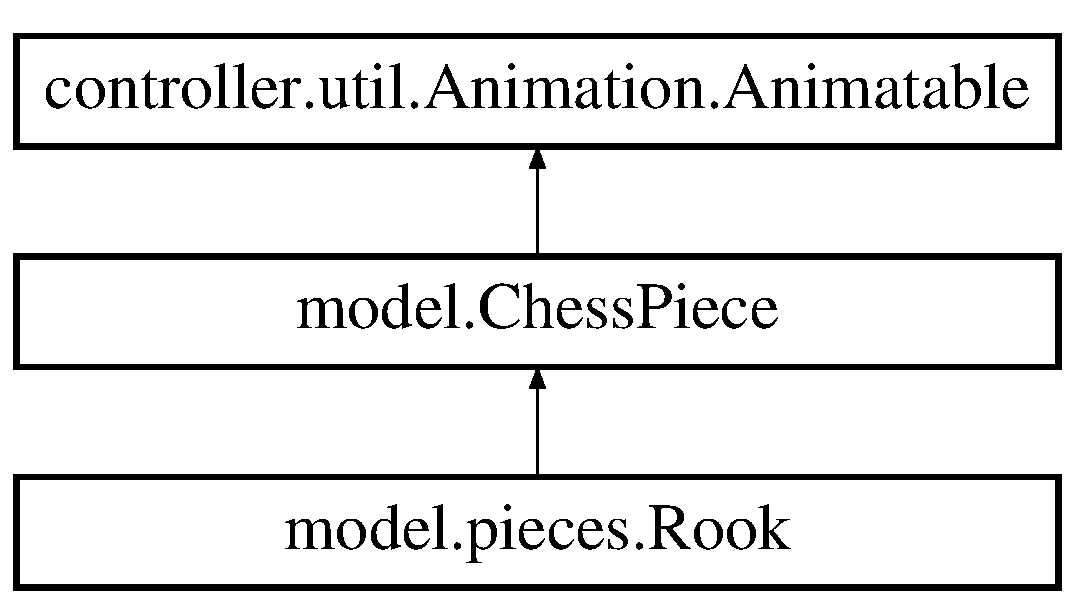
\includegraphics[height=3.000000cm]{classmodel_1_1pieces_1_1_rook}
\end{center}
\end{figure}
\subsection*{Public Member Functions}
\begin{DoxyCompactItemize}
\item 
\hypertarget{classmodel_1_1pieces_1_1_rook_a68e710f46abbb010f7c260a0336143b5}{{\bfseries Rook} (int x, int y, \hyperlink{classmodel_1_1board_1_1_board}{Board} \-\_\-board, \hyperlink{classcontroller_1_1_player}{Player} \-\_\-player)}\label{classmodel_1_1pieces_1_1_rook_a68e710f46abbb010f7c260a0336143b5}

\item 
Array\-List$<$ \hyperlink{classmodel_1_1_chess_move}{Chess\-Move} $>$ \hyperlink{classmodel_1_1pieces_1_1_rook_acdc88fcdbb81116be30b7f8c8c39e735}{get\-Possible\-Moves} ()
\item 
String \hyperlink{classmodel_1_1pieces_1_1_rook_a4ff4e4b36a743af9b64de9b53a9e1535}{get\-Type} ()
\end{DoxyCompactItemize}
\subsection*{Additional Inherited Members}


\subsection{Detailed Description}
Represents a \hyperlink{classmodel_1_1pieces_1_1_rook}{Rook}

\begin{DoxyAuthor}{Author}
Nicholas 
\end{DoxyAuthor}


\subsection{Member Function Documentation}
\hypertarget{classmodel_1_1pieces_1_1_rook_acdc88fcdbb81116be30b7f8c8c39e735}{\index{model\-::pieces\-::\-Rook@{model\-::pieces\-::\-Rook}!get\-Possible\-Moves@{get\-Possible\-Moves}}
\index{get\-Possible\-Moves@{get\-Possible\-Moves}!model::pieces::Rook@{model\-::pieces\-::\-Rook}}
\subsubsection[{get\-Possible\-Moves}]{\setlength{\rightskip}{0pt plus 5cm}Array\-List$<${\bf Chess\-Move}$>$ model.\-pieces.\-Rook.\-get\-Possible\-Moves (
\begin{DoxyParamCaption}
{}
\end{DoxyParamCaption}
)\hspace{0.3cm}{\ttfamily [virtual]}}}\label{classmodel_1_1pieces_1_1_rook_acdc88fcdbb81116be30b7f8c8c39e735}
Returns all the rank-\/file moves that the bishop can capture/move 

Implements \hyperlink{classmodel_1_1_chess_piece_a39d690c52727de4a27d2faee4e8b1ac7}{model.\-Chess\-Piece}.

\hypertarget{classmodel_1_1pieces_1_1_rook_a4ff4e4b36a743af9b64de9b53a9e1535}{\index{model\-::pieces\-::\-Rook@{model\-::pieces\-::\-Rook}!get\-Type@{get\-Type}}
\index{get\-Type@{get\-Type}!model::pieces::Rook@{model\-::pieces\-::\-Rook}}
\subsubsection[{get\-Type}]{\setlength{\rightskip}{0pt plus 5cm}String model.\-pieces.\-Rook.\-get\-Type (
\begin{DoxyParamCaption}
{}
\end{DoxyParamCaption}
)\hspace{0.3cm}{\ttfamily [virtual]}}}\label{classmodel_1_1pieces_1_1_rook_a4ff4e4b36a743af9b64de9b53a9e1535}
Used to determine a pieces type without using reflection (ie instanceof)

\begin{DoxyReturn}{Returns}
A string that contains the name of the piece, ie the \hyperlink{classmodel_1_1pieces_1_1_pawn}{Pawn} class would return \char`\"{}\-Pawn\char`\"{} 
\end{DoxyReturn}


Implements \hyperlink{classmodel_1_1_chess_piece_a68308e2fa0fe868f7386d40c6cd925df}{model.\-Chess\-Piece}.



The documentation for this class was generated from the following file\-:\begin{DoxyCompactItemize}
\item 
src/model/pieces/Rook.\-java\end{DoxyCompactItemize}

\hypertarget{classview_1_1loaders_1_1structures_1_1_shader}{\section{view.\-loaders.\-structures.\-Shader Class Reference}
\label{classview_1_1loaders_1_1structures_1_1_shader}\index{view.\-loaders.\-structures.\-Shader@{view.\-loaders.\-structures.\-Shader}}
}
\subsection*{Public Member Functions}
\begin{DoxyCompactItemize}
\item 
\hypertarget{classview_1_1loaders_1_1structures_1_1_shader_a9b3ac42119b7684612619a4a86dfab35}{{\bfseries Shader} (G\-L2 gl, File vs, File fs)  throws I\-O\-Exception }\label{classview_1_1loaders_1_1structures_1_1_shader_a9b3ac42119b7684612619a4a86dfab35}

\item 
\hypertarget{classview_1_1loaders_1_1structures_1_1_shader_ac44d55137349cf0b7a00446ecf3ff8f9}{void {\bfseries use\-Shader} (G\-L2 gl)}\label{classview_1_1loaders_1_1structures_1_1_shader_ac44d55137349cf0b7a00446ecf3ff8f9}

\end{DoxyCompactItemize}


\subsection{Detailed Description}
\hyperlink{classview_1_1loaders_1_1structures_1_1_shader}{Shader} class that represents an opengl shader, ie a vertex and fragment shader.

Currently this is not used

\begin{DoxyAuthor}{Author}
Nicholas 
\end{DoxyAuthor}


The documentation for this class was generated from the following file\-:\begin{DoxyCompactItemize}
\item 
src/view/loaders/structures/Shader.\-java\end{DoxyCompactItemize}

\hypertarget{classmodel_1_1game__modes_1_1_standard_game}{\section{model.\-game\-\_\-modes.\-Standard\-Game Class Reference}
\label{classmodel_1_1game__modes_1_1_standard_game}\index{model.\-game\-\_\-modes.\-Standard\-Game@{model.\-game\-\_\-modes.\-Standard\-Game}}
}
Inheritance diagram for model.\-game\-\_\-modes.\-Standard\-Game\-:\begin{figure}[H]
\begin{center}
\leavevmode
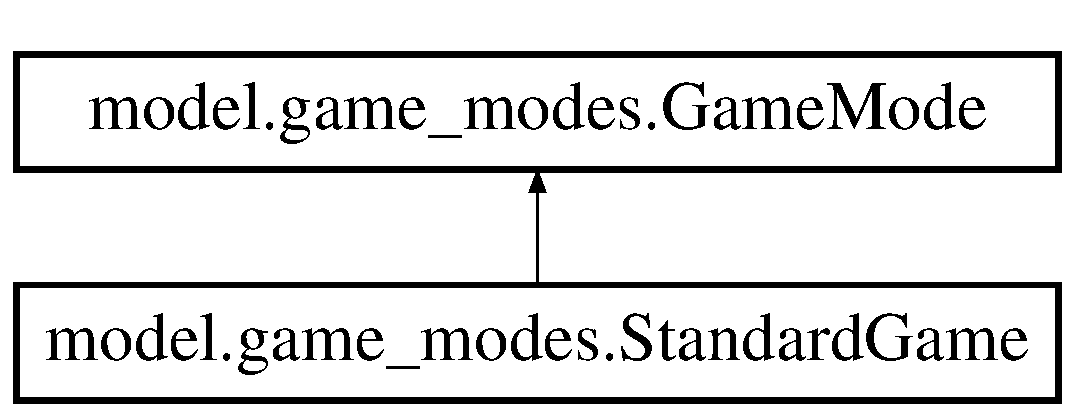
\includegraphics[height=2.000000cm]{classmodel_1_1game__modes_1_1_standard_game}
\end{center}
\end{figure}
\subsection*{Public Member Functions}
\begin{DoxyCompactItemize}
\item 
\hyperlink{classmodel_1_1board_1_1_board}{Board} \hyperlink{classmodel_1_1game__modes_1_1_standard_game_af204c61bdf19a90aeef707435a65a4b0}{init\-Pieces} (\hyperlink{classcontroller_1_1_player}{Player} player1, \hyperlink{classcontroller_1_1_player}{Player} player2)
\item 
boolean \hyperlink{classmodel_1_1game__modes_1_1_standard_game_a532a81128fd4292f85774d2ec383bbe5}{board\-Valid} (\hyperlink{classmodel_1_1board_1_1_board}{Board} board, \hyperlink{classcontroller_1_1_player}{Player} mover, \hyperlink{classmodel_1_1_chess_move}{Chess\-Move} last\-Move)
\item 
boolean \hyperlink{classmodel_1_1game__modes_1_1_standard_game_af859966b1b11825d30292cc9a6adf3e4}{has\-Player\-Lost} (\hyperlink{classmodel_1_1board_1_1_board}{Board} board, \hyperlink{classcontroller_1_1_player}{Player} victim)
\item 
void \hyperlink{classmodel_1_1game__modes_1_1_standard_game_ac71e444bda1320574ddf4be97724dbb6}{post\-Move\-Action} (final \hyperlink{classcontroller_1_1_game_loop}{Game\-Loop} game\-Controller, \hyperlink{classmodel_1_1_chess_move}{Chess\-Move} last\-Move)
\end{DoxyCompactItemize}


\subsection{Detailed Description}
Defines a \hyperlink{classmodel_1_1game__modes_1_1_standard_game}{Standard\-Game}, where the board is rectangular and the king cannot be in check.

\begin{DoxyAuthor}{Author}
Nicholas 
\end{DoxyAuthor}


\subsection{Member Function Documentation}
\hypertarget{classmodel_1_1game__modes_1_1_standard_game_a532a81128fd4292f85774d2ec383bbe5}{\index{model\-::game\-\_\-modes\-::\-Standard\-Game@{model\-::game\-\_\-modes\-::\-Standard\-Game}!board\-Valid@{board\-Valid}}
\index{board\-Valid@{board\-Valid}!model::game_modes::StandardGame@{model\-::game\-\_\-modes\-::\-Standard\-Game}}
\subsubsection[{board\-Valid}]{\setlength{\rightskip}{0pt plus 5cm}boolean model.\-game\-\_\-modes.\-Standard\-Game.\-board\-Valid (
\begin{DoxyParamCaption}
\item[{{\bf Board}}]{board, }
\item[{{\bf Player}}]{mover, }
\item[{{\bf Chess\-Move}}]{last\-Move}
\end{DoxyParamCaption}
)}}\label{classmodel_1_1game__modes_1_1_standard_game_a532a81128fd4292f85774d2ec383bbe5}
In a standard game this board is inspected to make sure the king is not in check \begin{DoxyReturn}{Returns}
true if the king is not in check, false otherwise; 
\end{DoxyReturn}


Implements \hyperlink{interfacemodel_1_1game__modes_1_1_game_mode_ab953f82866d9146bde4a2de96af7c308}{model.\-game\-\_\-modes.\-Game\-Mode}.

\hypertarget{classmodel_1_1game__modes_1_1_standard_game_af859966b1b11825d30292cc9a6adf3e4}{\index{model\-::game\-\_\-modes\-::\-Standard\-Game@{model\-::game\-\_\-modes\-::\-Standard\-Game}!has\-Player\-Lost@{has\-Player\-Lost}}
\index{has\-Player\-Lost@{has\-Player\-Lost}!model::game_modes::StandardGame@{model\-::game\-\_\-modes\-::\-Standard\-Game}}
\subsubsection[{has\-Player\-Lost}]{\setlength{\rightskip}{0pt plus 5cm}boolean model.\-game\-\_\-modes.\-Standard\-Game.\-has\-Player\-Lost (
\begin{DoxyParamCaption}
\item[{{\bf Board}}]{board, }
\item[{{\bf Player}}]{victim}
\end{DoxyParamCaption}
)}}\label{classmodel_1_1game__modes_1_1_standard_game_af859966b1b11825d30292cc9a6adf3e4}
Called when there are no moves left for the current player. At this point the game will be a stalemate or a player has lost.


\begin{DoxyParams}{Parameters}
{\em board} & \\
\hline
{\em victim} & \\
\hline
\end{DoxyParams}
\begin{DoxyReturn}{Returns}
true if the player has lost, false if it is a stalemate 
\end{DoxyReturn}


Implements \hyperlink{interfacemodel_1_1game__modes_1_1_game_mode_adaba2585b6c82e7e14532692db14898f}{model.\-game\-\_\-modes.\-Game\-Mode}.

\hypertarget{classmodel_1_1game__modes_1_1_standard_game_af204c61bdf19a90aeef707435a65a4b0}{\index{model\-::game\-\_\-modes\-::\-Standard\-Game@{model\-::game\-\_\-modes\-::\-Standard\-Game}!init\-Pieces@{init\-Pieces}}
\index{init\-Pieces@{init\-Pieces}!model::game_modes::StandardGame@{model\-::game\-\_\-modes\-::\-Standard\-Game}}
\subsubsection[{init\-Pieces}]{\setlength{\rightskip}{0pt plus 5cm}{\bf Board} model.\-game\-\_\-modes.\-Standard\-Game.\-init\-Pieces (
\begin{DoxyParamCaption}
\item[{{\bf Player}}]{player1, }
\item[{{\bf Player}}]{player2}
\end{DoxyParamCaption}
)}}\label{classmodel_1_1game__modes_1_1_standard_game_af204c61bdf19a90aeef707435a65a4b0}
Creates a board object with the players passed in. This method will return a complete setup based on the \hyperlink{interfacemodel_1_1game__modes_1_1_game_mode}{Game\-Mode}


\begin{DoxyParams}{Parameters}
{\em player1} & \\
\hline
{\em player2} & \\
\hline
\end{DoxyParams}
\begin{DoxyReturn}{Returns}
Board that has been setup with the rules of the \hyperlink{interfacemodel_1_1game__modes_1_1_game_mode}{Game\-Mode} 
\end{DoxyReturn}


Implements \hyperlink{interfacemodel_1_1game__modes_1_1_game_mode_a237818232e386862838f6b507299497b}{model.\-game\-\_\-modes.\-Game\-Mode}.

\hypertarget{classmodel_1_1game__modes_1_1_standard_game_ac71e444bda1320574ddf4be97724dbb6}{\index{model\-::game\-\_\-modes\-::\-Standard\-Game@{model\-::game\-\_\-modes\-::\-Standard\-Game}!post\-Move\-Action@{post\-Move\-Action}}
\index{post\-Move\-Action@{post\-Move\-Action}!model::game_modes::StandardGame@{model\-::game\-\_\-modes\-::\-Standard\-Game}}
\subsubsection[{post\-Move\-Action}]{\setlength{\rightskip}{0pt plus 5cm}void model.\-game\-\_\-modes.\-Standard\-Game.\-post\-Move\-Action (
\begin{DoxyParamCaption}
\item[{final {\bf Game\-Loop}}]{game\-Controller, }
\item[{{\bf Chess\-Move}}]{last\-Move}
\end{DoxyParamCaption}
)}}\label{classmodel_1_1game__modes_1_1_standard_game_ac71e444bda1320574ddf4be97724dbb6}
Called after a move has been executed. This method should display and warning, such as check in a Standard game


\begin{DoxyParams}{Parameters}
{\em game\-Controller} & \\
\hline
{\em last\-Move} & \\
\hline
\end{DoxyParams}


Implements \hyperlink{interfacemodel_1_1game__modes_1_1_game_mode_a034774ac426a436f2c19e7afc8eb8747}{model.\-game\-\_\-modes.\-Game\-Mode}.



The documentation for this class was generated from the following file\-:\begin{DoxyCompactItemize}
\item 
src/model/game\-\_\-modes/Standard\-Game.\-java\end{DoxyCompactItemize}

\hypertarget{classtests_1_1_standard_game_simulation_test}{\section{tests.\-Standard\-Game\-Simulation\-Test Class Reference}
\label{classtests_1_1_standard_game_simulation_test}\index{tests.\-Standard\-Game\-Simulation\-Test@{tests.\-Standard\-Game\-Simulation\-Test}}
}
\subsection*{Static Public Member Functions}
\begin{DoxyCompactItemize}
\item 
\hypertarget{classtests_1_1_standard_game_simulation_test_ac9b95ee7d33b13900839daf5ade8657e}{static void {\bfseries main} (String\mbox{[}$\,$\mbox{]} args)}\label{classtests_1_1_standard_game_simulation_test_ac9b95ee7d33b13900839daf5ade8657e}

\end{DoxyCompactItemize}


\subsection{Detailed Description}
Simulates a (short) chess game that results in black checkmated. Demonstrates the G\-U\-I.

\begin{DoxyAuthor}{Author}
Nicholas 
\end{DoxyAuthor}


The documentation for this class was generated from the following file\-:\begin{DoxyCompactItemize}
\item 
src/tests/Standard\-Game\-Simulation\-Test.\-java\end{DoxyCompactItemize}

\hypertarget{classtests_1_1_standard_game_test}{\section{tests.\-Standard\-Game\-Test Class Reference}
\label{classtests_1_1_standard_game_test}\index{tests.\-Standard\-Game\-Test@{tests.\-Standard\-Game\-Test}}
}
\subsection*{Static Public Member Functions}
\begin{DoxyCompactItemize}
\item 
\hypertarget{classtests_1_1_standard_game_test_a72a09f86c1d5cb86b2ccf1d0252d67b4}{static void {\bfseries main} (String\mbox{[}$\,$\mbox{]} args)}\label{classtests_1_1_standard_game_test_a72a09f86c1d5cb86b2ccf1d0252d67b4}

\end{DoxyCompactItemize}


\subsection{Detailed Description}
Simulates a Standard\-Game with the G\-U\-I

\begin{DoxyAuthor}{Author}
Nicholas 
\end{DoxyAuthor}


The documentation for this class was generated from the following file\-:\begin{DoxyCompactItemize}
\item 
src/tests/Standard\-Game\-Test.\-java\end{DoxyCompactItemize}

\hypertarget{classtests_1_1core__tests_1_1_test_check_senerios}{\section{tests.\-core\-\_\-tests.\-Test\-Check\-Senerios Class Reference}
\label{classtests_1_1core__tests_1_1_test_check_senerios}\index{tests.\-core\-\_\-tests.\-Test\-Check\-Senerios@{tests.\-core\-\_\-tests.\-Test\-Check\-Senerios}}
}
\subsection*{Public Member Functions}
\begin{DoxyCompactItemize}
\item 
\hypertarget{classtests_1_1core__tests_1_1_test_check_senerios_aa981055645645028d13db1f3c5d850ac}{void {\bfseries setup} ()}\label{classtests_1_1core__tests_1_1_test_check_senerios_aa981055645645028d13db1f3c5d850ac}

\item 
void \hyperlink{classtests_1_1core__tests_1_1_test_check_senerios_aefce5843fbe7952185c64888b1230bd3}{test\-Basic\-Check} ()
\item 
void \hyperlink{classtests_1_1core__tests_1_1_test_check_senerios_a36b95cc47e92104189d6e1829488b002}{test\-Basic\-No\-Check} ()
\item 
void \hyperlink{classtests_1_1core__tests_1_1_test_check_senerios_a0538efdd54699e0b81cea9af1af80d54}{test\-Complicated\-Check} ()
\item 
void \hyperlink{classtests_1_1core__tests_1_1_test_check_senerios_a12554781faa512dd4b086263778e537b}{test\-Complicated\-Mate} ()
\end{DoxyCompactItemize}


\subsection{Detailed Description}
Checks various check/checkmate scenarios

\begin{DoxyAuthor}{Author}
Nicholas 
\end{DoxyAuthor}


\subsection{Member Function Documentation}
\hypertarget{classtests_1_1core__tests_1_1_test_check_senerios_aefce5843fbe7952185c64888b1230bd3}{\index{tests\-::core\-\_\-tests\-::\-Test\-Check\-Senerios@{tests\-::core\-\_\-tests\-::\-Test\-Check\-Senerios}!test\-Basic\-Check@{test\-Basic\-Check}}
\index{test\-Basic\-Check@{test\-Basic\-Check}!tests::core_tests::TestCheckSenerios@{tests\-::core\-\_\-tests\-::\-Test\-Check\-Senerios}}
\subsubsection[{test\-Basic\-Check}]{\setlength{\rightskip}{0pt plus 5cm}void tests.\-core\-\_\-tests.\-Test\-Check\-Senerios.\-test\-Basic\-Check (
\begin{DoxyParamCaption}
{}
\end{DoxyParamCaption}
)}}\label{classtests_1_1core__tests_1_1_test_check_senerios_aefce5843fbe7952185c64888b1230bd3}
Tests to see if a bishop at 4,4 causes check to a king at 2,2 \hypertarget{classtests_1_1core__tests_1_1_test_check_senerios_a36b95cc47e92104189d6e1829488b002}{\index{tests\-::core\-\_\-tests\-::\-Test\-Check\-Senerios@{tests\-::core\-\_\-tests\-::\-Test\-Check\-Senerios}!test\-Basic\-No\-Check@{test\-Basic\-No\-Check}}
\index{test\-Basic\-No\-Check@{test\-Basic\-No\-Check}!tests::core_tests::TestCheckSenerios@{tests\-::core\-\_\-tests\-::\-Test\-Check\-Senerios}}
\subsubsection[{test\-Basic\-No\-Check}]{\setlength{\rightskip}{0pt plus 5cm}void tests.\-core\-\_\-tests.\-Test\-Check\-Senerios.\-test\-Basic\-No\-Check (
\begin{DoxyParamCaption}
{}
\end{DoxyParamCaption}
)}}\label{classtests_1_1core__tests_1_1_test_check_senerios_a36b95cc47e92104189d6e1829488b002}
Same scenario as \hyperlink{classtests_1_1core__tests_1_1_test_check_senerios_aefce5843fbe7952185c64888b1230bd3}{test\-Basic\-Check()} but with a friendly pawn in between so no check should be available \hypertarget{classtests_1_1core__tests_1_1_test_check_senerios_a0538efdd54699e0b81cea9af1af80d54}{\index{tests\-::core\-\_\-tests\-::\-Test\-Check\-Senerios@{tests\-::core\-\_\-tests\-::\-Test\-Check\-Senerios}!test\-Complicated\-Check@{test\-Complicated\-Check}}
\index{test\-Complicated\-Check@{test\-Complicated\-Check}!tests::core_tests::TestCheckSenerios@{tests\-::core\-\_\-tests\-::\-Test\-Check\-Senerios}}
\subsubsection[{test\-Complicated\-Check}]{\setlength{\rightskip}{0pt plus 5cm}void tests.\-core\-\_\-tests.\-Test\-Check\-Senerios.\-test\-Complicated\-Check (
\begin{DoxyParamCaption}
{}
\end{DoxyParamCaption}
)}}\label{classtests_1_1core__tests_1_1_test_check_senerios_a0538efdd54699e0b81cea9af1af80d54}
Tests a complicated check situation where the king can only move in 2 possible locations. A queen is then added, to opening another option to avoid check by moving the Queen in front of the bishop \hypertarget{classtests_1_1core__tests_1_1_test_check_senerios_a12554781faa512dd4b086263778e537b}{\index{tests\-::core\-\_\-tests\-::\-Test\-Check\-Senerios@{tests\-::core\-\_\-tests\-::\-Test\-Check\-Senerios}!test\-Complicated\-Mate@{test\-Complicated\-Mate}}
\index{test\-Complicated\-Mate@{test\-Complicated\-Mate}!tests::core_tests::TestCheckSenerios@{tests\-::core\-\_\-tests\-::\-Test\-Check\-Senerios}}
\subsubsection[{test\-Complicated\-Mate}]{\setlength{\rightskip}{0pt plus 5cm}void tests.\-core\-\_\-tests.\-Test\-Check\-Senerios.\-test\-Complicated\-Mate (
\begin{DoxyParamCaption}
{}
\end{DoxyParamCaption}
)}}\label{classtests_1_1core__tests_1_1_test_check_senerios_a12554781faa512dd4b086263778e537b}
Tests a complicated checkmate situation where player2 is checkmated by player1's knight. 

The documentation for this class was generated from the following file\-:\begin{DoxyCompactItemize}
\item 
src/tests/core\-\_\-tests/Test\-Check\-Senerios.\-java\end{DoxyCompactItemize}

\hypertarget{classtests_1_1core__tests_1_1_test_moves}{\section{tests.\-core\-\_\-tests.\-Test\-Moves Class Reference}
\label{classtests_1_1core__tests_1_1_test_moves}\index{tests.\-core\-\_\-tests.\-Test\-Moves@{tests.\-core\-\_\-tests.\-Test\-Moves}}
}
\subsection*{Public Member Functions}
\begin{DoxyCompactItemize}
\item 
\hypertarget{classtests_1_1core__tests_1_1_test_moves_a45c2007c0c18c40280ab2aba52293d56}{void {\bfseries setup} ()}\label{classtests_1_1core__tests_1_1_test_moves_a45c2007c0c18c40280ab2aba52293d56}

\item 
\hypertarget{classtests_1_1core__tests_1_1_test_moves_abbcc229dd74d12b55bb5470c6cde83d5}{void {\bfseries test\-Rectangular\-Board\-Methods} ()}\label{classtests_1_1core__tests_1_1_test_moves_abbcc229dd74d12b55bb5470c6cde83d5}

\item 
\hypertarget{classtests_1_1core__tests_1_1_test_moves_a098c97c200f9732a6f09626c0989e18f}{void {\bfseries test\-Pawn\-Moves} ()}\label{classtests_1_1core__tests_1_1_test_moves_a098c97c200f9732a6f09626c0989e18f}

\item 
\hypertarget{classtests_1_1core__tests_1_1_test_moves_a04469a1b9ecb3e79c921ff3aec591762}{void {\bfseries test\-Knight\-Moves} ()}\label{classtests_1_1core__tests_1_1_test_moves_a04469a1b9ecb3e79c921ff3aec591762}

\item 
\hypertarget{classtests_1_1core__tests_1_1_test_moves_a528360fefa052fe07af851698946c2a4}{void {\bfseries test\-Rook\-Moves} ()}\label{classtests_1_1core__tests_1_1_test_moves_a528360fefa052fe07af851698946c2a4}

\item 
\hypertarget{classtests_1_1core__tests_1_1_test_moves_a6e73b340a03033e42d2259bb6936a1e6}{void {\bfseries test\-Bishop\-Moves} ()}\label{classtests_1_1core__tests_1_1_test_moves_a6e73b340a03033e42d2259bb6936a1e6}

\item 
\hypertarget{classtests_1_1core__tests_1_1_test_moves_a7c85d3ad6f95e18e89742959d6800c57}{void {\bfseries test\-Queen\-Moves} ()}\label{classtests_1_1core__tests_1_1_test_moves_a7c85d3ad6f95e18e89742959d6800c57}

\item 
\hypertarget{classtests_1_1core__tests_1_1_test_moves_a9e4e775400a68f01cc2f61f3f7dbae1a}{void {\bfseries test\-King\-Moves} ()}\label{classtests_1_1core__tests_1_1_test_moves_a9e4e775400a68f01cc2f61f3f7dbae1a}

\item 
\hypertarget{classtests_1_1core__tests_1_1_test_moves_a1402021b36f732856fc6007df754f143}{void {\bfseries test\-Lame\-Queen\-Moves} ()}\label{classtests_1_1core__tests_1_1_test_moves_a1402021b36f732856fc6007df754f143}

\item 
\hypertarget{classtests_1_1core__tests_1_1_test_moves_a27dd9dabc0a99b27e53a2d00dbd61134}{void {\bfseries test\-Chancellor\-Moves} ()}\label{classtests_1_1core__tests_1_1_test_moves_a27dd9dabc0a99b27e53a2d00dbd61134}

\end{DoxyCompactItemize}


\subsection{Detailed Description}
These tests test the functionality of the Board, and the various chess pieces.

\begin{DoxyAuthor}{Author}
Nicholas 
\end{DoxyAuthor}


The documentation for this class was generated from the following file\-:\begin{DoxyCompactItemize}
\item 
src/tests/core\-\_\-tests/Test\-Moves.\-java\end{DoxyCompactItemize}

\hypertarget{classtests_1_1core__tests_1_1_test_suite}{\section{tests.\-core\-\_\-tests.\-Test\-Suite Class Reference}
\label{classtests_1_1core__tests_1_1_test_suite}\index{tests.\-core\-\_\-tests.\-Test\-Suite@{tests.\-core\-\_\-tests.\-Test\-Suite}}
}


The documentation for this class was generated from the following file\-:\begin{DoxyCompactItemize}
\item 
src/tests/core\-\_\-tests/Test\-Suite.\-java\end{DoxyCompactItemize}

\hypertarget{classtests_1_1core__tests_1_1_test_undo}{\section{tests.\-core\-\_\-tests.\-Test\-Undo Class Reference}
\label{classtests_1_1core__tests_1_1_test_undo}\index{tests.\-core\-\_\-tests.\-Test\-Undo@{tests.\-core\-\_\-tests.\-Test\-Undo}}
}
\subsection*{Public Member Functions}
\begin{DoxyCompactItemize}
\item 
\hypertarget{classtests_1_1core__tests_1_1_test_undo_a12206580643377499c929d7d80a1d15a}{void {\bfseries setup} ()}\label{classtests_1_1core__tests_1_1_test_undo_a12206580643377499c929d7d80a1d15a}

\item 
\hypertarget{classtests_1_1core__tests_1_1_test_undo_aa8b1e68de7ca34af33adbbce703d6191}{void {\bfseries test\-Basic\-Undo\-Methods} ()}\label{classtests_1_1core__tests_1_1_test_undo_aa8b1e68de7ca34af33adbbce703d6191}

\item 
\hypertarget{classtests_1_1core__tests_1_1_test_undo_a279a9cab8ec841ef5f5b4d2ca6840bfa}{void {\bfseries test\-Capture\-Undo\-Methods} ()}\label{classtests_1_1core__tests_1_1_test_undo_a279a9cab8ec841ef5f5b4d2ca6840bfa}

\end{DoxyCompactItemize}


The documentation for this class was generated from the following file\-:\begin{DoxyCompactItemize}
\item 
src/tests/core\-\_\-tests/Test\-Undo.\-java\end{DoxyCompactItemize}

%--- End generated contents ---

% Index
\newpage
\phantomsection
\addcontentsline{toc}{part}{Index}
\printindex

\end{document}
